% \chapter{Introduction}

\green{}

The Swarm project is set out to build permissionless storage and communication infrastructure for tomorrow's self-sovereign digital society. From a developer's perspective, Swarm is best seen as public infrastructure that powers real-time interactive web applications familiar from the \gloss{Web 2.0} era. It provides low-level API to primitives that serve as building blocks of complex applications as well as the basis for the tools and libraries for a Swarm-based \gloss{Web 3.0} development stack. The API and the tools let Swarm be used in the browser, so Swarm can act as a decentralised alternative to today's \gloss{World Wide Web}.

This part details the design and architecture of the system. In accordance with the principles laid out in \ref{sec:design-principles}, we put an emphasis on modular design, and conceive of Swarm as having clearly separable layers (see figure \ref{fig:Swarm-layered-design}), each dependent on the previous one: (1) a peer-to-peer network protocol to serve as underlay transport, (2) an overlay network with protocols powering a distributed immutable storage of \glossplural{chunk} (fix-sized data blocks), (3) a component for higher-level data access defining APIs for the base-layer features, and (4) an application layer potentially defining the standards, capturing best practices for more elaborate use-cases. We regard (2) and (3) as the core of Swarm. Since the network layer relies on it we formulate the requirements for (1), but we consider the detailed treatment of both (1) and (4) outside the scope of this book.


\begin{figure}[htbp]
  \centering
  \caption[Swarm's layered design]{Swarm's layered design}
  \label{fig:Swarm-layered-design}
\end{figure}

Central to the design, the architecture of Swarm overlay network (layer 2 in figure \ref{fig:Swarm-layered-design}) is discussed in chapter \ref{sec:network} and is complemented by chapter \ref{sec:incentivisation}, describing the system of economic incentives which makes Swarm self-sustaining. In chapter \ref{sec:high-level-functionality}, we introduce the algorithms and conventions that allow Swarm to map data concepts onto the chunk layer to enable high-level functionality for storage and communication, notably data structures, access control, feeds, direct messaging and persistence (layer 3 in figure \ref{fig:Swarm-layered-design}).
In chapter \ref{sec:persistence}, we present ways to prevent garbage collected chunks from disappearing, including: \gloss{erasure code}, pinning and insurance, and also provide ways to recover and reupload them using missing chunk notifications or insurance challenges. 
Finally, chapter \ref{sec:ux} looks at functionality from a user experience perspective.

\chapter{Network}\label{sec:network}

This chapter offers a narrative on how the Swarm overlay network is built on top of a \gloss{peer-to-peer} network protocol and forms a topology that allows for routing of messages between nodes (\ref{sec:topology-routing}). In \ref{sec:kademlia-storage}, we describe how such a network can serve as a scalable \gloss{distributed storage} solution for chunks (\ref{sec:chunks}) and present the logic behind the protocols for retrieval/download and \gloss{syncing}/upload (\ref{sec:push-and-pull}).

\section{Topology and routing}\label{sec:topology-routing}

This section sets the scene (\ref{sec:underlay-transport}) for the \gloss{overlay network} (layer 2) of Swarm by making explicit the assumptions about the underlay transport (layer 1). \ref{sec:overlay-addressing} introduces the \gloss{overlay address space} and explains how nodes are assigned an address. In  \ref{sec:kademlia-routing}, we present the \gloss{Kademlia} \gloss{overlay topology} (connectivity pattern) and explain how it solves routing between nodes. In \ref{sec:bootstrapping} we show how nodes running the Swarm client can discover each other, bootstrap and maintain the overlay topology.

\subsection{Requirements for underlay transport}\label{sec:underlay-transport} 

\yellow{}

Swarm is a network operated by its users. Each node in the network is supposed to run a client complying with the protocol specifications. On the lowest level, the nodes in the network connect using a peer-to-peer network protocol as their transport layer. This is called the \gloss{underlay network}. 
In its overall design, Swarm is agnostic of the particular underlay transport used as long as it satisfies the following requirements.

\begin{enumerate}
    \item \emph{addressing} - Nodes are identified by their \gloss{underlay address}.
    \item \emph{dialling} - Nodes can initiate a direct connection to a peer by dialing them on their underlay address.
    \item \emph{listening} - Nodes can listen to other peers dialing them and can accept incoming connections.
    \item \emph{live connection} - A node connection establishes a channel of communication which is kept alive until explicit disconnection, so that the existence of a connection means the remote peer is online and accepting messages.
    \item \emph{channel security} - 
    The channel provides identity verification and implements encrypted and authenticated transport resisting man in the middle attacks.
    \item \emph{protocol multiplexing} - 
    The underlay network service can accommodate several protocols running on the same connection. Peers communicate the protocols (with name and versions) they implement and the underlay service identifies compatible protocols and starts up peer connections on each matched protocol. 
    \item \emph{delivery guarantees} - 
    Protocol messages have \gloss{guaranteed delivery}, i.e., delivery failures due to network problems result in direct error response. 
    Order of delivery of messages within each protocol is guaranteed. 
    Ideally the underlay protocol provides prioritisation. 
    If protocol multiplexing is over the same transport channel, this most likely implies framing so that long messages do not block higher priority messages.
    \item \emph{serialisation} - 
    The protocol message construction supports arbitrary data structure serialisation conventions.
    
\end{enumerate}

The \gloss{libp2p} library provides all the needed functionality and is the one given in the specification as underlay connectivity driver, see \ref{spec:protocol:intro}.%
%
\footnote{Swarm's current golang implementation uses Ethereum's \gloss{devp2p}/rlpx which satisfies the above criteria and uses TCP/IP with custom cryptography added for security. The underlay network address devp2p uses is represented using the \gloss{enode} url scheme. Devp2p dispatches protocol messages based on their message ID. It uses RLP serialisation which is extended with higher level data type representation conventions. In order to provide support for Ethereum 1.x blockchain and state on Swarm, we may provide a thin devp2p node that proxies queries to a libp2p-based Swarn client or just uses its API. Otherwise we see the devp2p networking support discontinued.}

\subsection{Overlay addressing}\label{sec:overlay-addressing} 
\green{}

While clients use the \gloss{underlay address} to establish connections to peers, each node running Swarm is additionally identified with an \gloss{overlay address}. It is this address that determines which peers a node will connect to and drives the way messages are forwarded. The overlay address is assumed to be stable as it defines a node's identity across sessions and ultimately affects what content is most worth storing in the node's local storage.

The node's \gloss{overlay address} is derived from an Ethereum account by hashing the corresponding elliptic curve public key with the \gloss{BZZ network ID}, using 256-bit Keccak Sha3 (see \ref{spec:format:bzzaddress}). The BZZ network ID stems from the fact that there can be several Swarm networks (e.g., test net, main net, or private Swarms). The BZZ network ID makes it impossible to use the same address across networks. Assuming any sample of base accounts independently selected, the resulting overlay addresses are expected to have a uniform distribution in the address space of 256-bit integers. Deriving the address from a public key is important as it allows the nodes to issue commitments associated with an overlay location using signatures verifiable by 3rd parties. 

Using the long-lived communication channels of the \gloss{underlay network}, Swarm nodes are forming a network with \emph{quasi-permanent} peer connections. The resulting connectivity graph can realise a particular topology defined over the address space. The \gloss{overlay topology} chosen is called \gloss{Kademlia}: It enables communication between any two arbitrary nodes in the Swarm network by providing a strategy to relay messages using only underlay peer connections. The protocol that describes how nodes share information with each other about themselves and other peers is described in \ref{spec:protocol:hive}. How nodes use this protocol to bootstrap the \gloss{overlay topology} is discussed in \ref{sec:bootstrapping}. The  theoretical basis for \gloss{Kademlia topology} is formalised rigorously in \ref{sec:kademlia-connectivity}. 

Crucially, the overlay address space is 256-bit integers. Central to swarm is the notion of \gloss{proximity order} (\gloss{PO}) which measures the relatedness of two addresses on  a discrete scale.%
%
\footnote{Proximity order is the discrete logarithmic scaling of proximity, which, in turn is the inverse of normalised XOR distance. See \ref{sec:proximity} for a formal definition.}
%
Given two addresses, $x$ and $y$, $\mathit{PO}(x,y)$ counts the matching bits in their binary representation starting from the most significant bit up to the first difference. The highest proximity order is therefore 256, designating the maximum relatedness, i.e., when $x=y$.

\subsection{Kademlia routing}\label{sec:kademlia-routing}
\yellow{rework together with appendix}

\glossupper{Kademlia topology} can be used for routing messages between nodes in a network using overlay addressing. It has excellent scalability as it allows for such a universal routing with both (1) the number of hops and (2) the number of peer connections maintained being logarithmic to the size of the network. 

In what follows, we show that two different relations over nodes can be used to support two flavours of routing, \emph{iterative/zooming} and \emph{recursive/forwarding}. Swarm's design crucially relies on the latter choice, the forwarding flavour. However, as both the peer-to-peer literature and existing systems are predominantly using the iterative flavour (see \cite{maymounkov2002kademlia,baumgart2007s,lua2005survey}), we consider it instructive to subsume the two flavours under the same abstraction and walk the reader through the two options.

\subsubsection{Iterative and forwarding Kademlia}

Let $R$ be an arbitrary binary relation over nodes in a network. Nodes that are in relation $R$ with a particular node $x$ are called \glossplural{peer} of $x$. Peers of $x$ can be indexed by their \gloss{proximity order} (\gloss{PO}) relative to $x$ (see \ref{sec:proximity}).
The equivalence classes of peers are called \glossplural{proximity order bin}, or just \glossplural{bin} for short. When arranged in bins, peers of $x$ are grouped in the \gloss{Kademlia table} of the node $x$ (see figure \ref{fig:kademlia-table}). 



\begin{figure}[htbp]
   \centering
    % not sure about these colours!
\definecolor{c1}{HTML}{FF7F00}
\definecolor{c2}{HTML}{048BA8}
\definecolor{c3}{HTML}{16DB93}
\definecolor{c4}{HTML}{EFEA5A}
\definecolor{c5}{HTML}{F29E4C}
\definecolor{c6}{HTML}{256EFF}
\definecolor{c7}{HTML}{46237A}

\scalebox{1.35}{
\begin{forest}
rt/.style={draw=black,line width=1pt},
peer/.style={draw=black!60,edge={black!60,line width=0.7pt}},
peerleaf/.style={edge={black!60,line width=0.7pt}},
self/.style={draw=black,fill=black,edge={black,line width=1pt}},
selfpeer/.style={draw=black,line width=1pt,edge={black,line width=1pt}},
unused/.style={draw=black!20,edge={black!20,line width=0.7pt}},
[{},rt,for tree={circle,draw, l sep=20pt}
  [{},selfpeer,edge label={node[midway,left] {0}}
    [{},peer,edge label={node[midway,left] {0}}
      [{},peer,edge label={node[midway,left] {0}}
        [{},unused,edge label={node[midway,left] {0}}]
        [{},peerleaf,fill=c1,draw=c1,edge label={node[midway,right] {1}}]
      ]
      [{},peer,edge label={node[midway,right] {1}}
        [{},peerleaf,fill=c2,draw=c2,edge label={node[midway,left] {0}}]
        [{},unused,edge label={node[midway,right] {1}}]
      ]
    ]
    [{},selfpeer,edge label={node[midway,right] {1}} 
      [{},selfpeer,edge label={node[midway,left] {0}}
        [{},peerleaf,fill=c3,draw=c3,edge label={node[midway,left] {0}}]
        [{},self,edge label={node[midway,right] {1}}]
      ]
      [{},peer,edge label={node[midway,right] {1}}
        [{},peerleaf,fill=c4,draw=c4,edge label={node[midway,left] {0}}]
        [{},peerleaf,fill=c5,draw=c5,edge label={node[midway,right] {1}}]
      ]
    ] 
  ]
  [{},peer,edge label={node[midway,right] {1}}
    [{},unused,edge label={node[midway,left] {0}}
      [{},unused,edge label={node[midway,left] {0}}
        [{},unused,edge label={node[midway,left] {0}}]
        [{},unused,edge label={node[midway,right] {1}}]
      ]
      [{},unused,edge label={node[midway,right] {1}}
        [{},unused,edge label={node[midway,left] {0}}]
        [{},unused,edge label={node[midway,right] {1}}]
      ]
    ]
    [{},peer,edge label={node[midway,right] {1}} 
      [{},peer,edge label={node[midway,left] {0}}
        [{},fill=c6,peerleaf,draw=c6,edge label={node[midway,left] {0}}]
        [{},unused,edge label={node[midway,right] {1}}]
      ]
      [{},peer,edge label={node[midway,right] {1}}
        [{},fill=c7,peerleaf,draw=c7,edge label={node[midway,left] {0}}]
        [{},unused,edge label={node[midway,right] {1}}]
      ]
    ]
  ] 
]
\end{forest}
}
    % not sure about these colours!
\definecolor{c1}{HTML}{FF7F00}
\definecolor{c2}{HTML}{048BA8}
\definecolor{c3}{HTML}{16DB93}
\definecolor{c4}{HTML}{EFEA5A}
\definecolor{c5}{HTML}{F29E4C}
\definecolor{c6}{HTML}{256EFF}
\definecolor{c7}{HTML}{46237A}

\scalebox{1.35}{
\begin{forest}
rt/.style={draw=black,line width=1pt},
peer/.style={draw=black!60,edge={black!60,line width=0.7pt}},
peerleaf/.style={edge={black!60,line width=0.7pt}},
self/.style={draw=black,fill=black,edge={black,line width=1pt}},
selfpeer/.style={draw=black,line width=1pt,edge={black,line width=1pt}},
unused/.style={draw=black!20,edge={black!20,line width=0.7pt}},
[{},rt,for tree={circle,draw, l sep=20pt}
  [{},selfpeer,edge label={node[midway,left] {0}}
    [{},selfpeer,edge label={node[midway,left] {0}}
      [{},selfpeer,edge label={node[midway,left] {0}}
        [{},self,edge label={node[midway,left] {0}}]
        [{},draw=c3,fill=c3,peerleaf,edge label={node[midway,right] {1}}]
      ]
      [{},peer,edge label={node[midway,right] {1}}
        [{},draw=c4,fill=c5,peerleaf,edge label={node[midway,left] {0}}]
        [{},draw=c4,fill=c4,peerleaf,edge label={node[midway,right] {1}}]
      ]
    ]
    [{},peer,edge label={node[midway,right] {1}} 
      [{},peer,edge label={node[midway,left] {0}}
        [{},draw=c1,fill=c1,peerleaf,edge label={node[midway,left] {0}}]
        [{},unused,edge label={node[midway,right] {1}}]
      ]
      [{},peer,edge label={node[midway,right] {1}}
        [{},unused,edge label={node[midway,left] {0}}]
        [{},draw=c2,fill=c2,peerleaf,edge label={node[midway,right] {1}}]
      ]
    ] 
  ]
  [{},peer,edge label={node[midway,right] {1}}
    [{},peer,edge label={node[midway,left] {0}}
      [{},peer,edge label={node[midway,left] {0}}
        [{},unused,edge label={node[midway,left] {0}}]
        [{},draw=c6,fill=c6,peerleaf,edge label={node[midway,right] {1}}]
      ]
      [{},peer,edge label={node[midway,right] {1}}
        [{},unused,edge label={node[midway,left] {0}}]
        [{},draw=c7,fill=c7,peerleaf,edge label={node[midway,right] {1}}]
      ]
    ]
    [{},unused,edge label={node[midway,right] {1}} 
      [{},unused,edge label={node[midway,left] {0}}
        [{},unused,edge label={node[midway,left] {0}}]
        [{},unused,edge label={node[midway,right] {1}}]
      ]
      [{},unused,edge label={node[midway,right] {1}}
        [{},unused,edge label={node[midway,left] {0}}]
        [{},unused,edge label={node[midway,right] {1}}]
      ]
    ]
  ] 
]
\end{forest}
}
   \caption[Kademlia table (recursive flavour)]{\gloss{Kademlia table} (recursive flavour):  peers of node $x$ partitioned into proximity order bins. Saturated Kademlia connectivity is 
   characterised by a live Kademlia table of directly connected TCP peers such that (1) there is at least $k$ peers in each bin up to but excluding saturation depth $d_x$ and (2) all the nodes in the entire network that would fall in a bin higher or equal to $d_x$ are actually peers of $x$. }
   \label{fig:kademlia-table}
\end{figure}

Node $x$ has a \gloss{saturated Kademlia table} if there is a $0\leq d_x\leq \mathit{maxPO}$ called \gloss{neighbourhood depth} such that (1) the node has at least one peer in each bin up to and excluding \gloss{PO} bin $d_x$ and (2) all nodes at least as near as $d_x$ (called the \gloss{nearest neighbours}) are peers of $x$. If each node in a network has a saturated Kademlia table, then we say that the network has \gloss{Kademlia topology}.

Let $R$ be the "know about" relation:  $x$ "knows about" $y$ if $x$ has both overlay and underlay address information on $y$. 
In the iterative Kademlia routing the \gloss{requestor node} iteratively extends its "know-about" graph. Using their \gloss{underlay address} the requestor node will contact peers they know are nearest the destination address for further peers (commonly using UDP), on each successive iteration the peers are at least one order closer to the destination (see figure \ref{fig:iterative-kademlia}). Because of the Kademlia criteria, the requestor will end up knowing about the destination node's underlay address and can establish direct communication with it. This iterative strategy%
%
\footnote{The iterative protocol is equivalent to the original Kademlia routing that is described in \cite{maymounkov2002kademlia}.
}
%
critically depends on the nodes' ability to find peers that are online. In order to find one, a node needs to collect several candidate peers for each bin. The best predictor of availability is the recency of the peer's last response, so peers in a \gloss{bin} should be prioritised according to this ordering.

\begin{figure}[htbp]
   \centering
   \caption[Iterative Kademlia routing]{TBD Iterative Kademlia routing}
   \label{fig:iterative-kademlia}
\end{figure}


An alternative flavour of Kademlia routing is described first in \cite{heep2010r} and worked out in \cite{tronetal2019-network}. Here, a recursive method is employed, whereby the successive steps of the iteration are "outsourced" to a \gloss{downstream peer}.
Each node recursively passes a message to a direct peer at least one \gloss{PO} closer to the destination. \glossupper{routing} here means relaying messages via a chain of peers ever closer to the destination.

Swarm's underlay transport offers quasi-stable peer connections (over TCP) with communication channels that are kept alive. Open connections can be used as $R$ to define another notion of \gloss{peer}. The two criteria of healthy \gloss{Kademlia connectivity} translate as: For each node $x$, there exists a \gloss{neighbourhood depth} $d_x$ such that (1) node $x$ has an open connection with at least one node for each \gloss{PO bin} up to but excluding $d_x$ and (2) connected to all the nodes at least as near as $d_x$. If each node in the network has a saturated Kademlia table of peers, then the network has \gloss{Kademlia topology}. Since connected peers are guaranteed to be online, the recursive step consists solely of forwarding the message to a connected peer strictly closer to the destination. We can call this alternative a \gloss{forwarding Kademlia} (see figure \ref{fig:forwarding-kademlia}). 


\begin{figure}[htbp]
   \centering
   \caption[Forwarding Kademlia routing]{TBD Forwarding Kademlia routing}
   \label{fig:forwarding-kademlia}
\end{figure}


In a \gloss{forwarding Kademlia} network, a message is said to be \emph{routable} if there exists a path from sender to destination through which the message could be relayed. In a mature subnetwork with \gloss{Kademlia topology} every message is routable. 

If all peer connections are stably online, a \gloss{thin Kademlia table}, i.e., a single \gloss{peer} for each \gloss{bin} up to $d$, is sufficient to guarantee routing between nodes. In reality, however, networks have \gloss{churn}, i.e., nodes are expected to go offline regularly. In order to ensure \gloss{routability} in the face of churn, the network needs to maintain \gloss{Kademlia topology}. This means that each individual node needs to have a \gloss{saturated Kademlia table} at all times. By keeping several connected peers in each \gloss{PO bin}, a node can ensure that node dropouts do not damage the saturation of their Kademlia table. Given a model of node dropouts, we can calculate the minimum number of peers needed per bin to guarantee that nodes are saturated with a probability arbitrarily close to 1. The more peers a node keeps in a PO bin, the longer the message destination address match the prefix of a peer. As a consequence of forwarding the message to that peer, the \gloss{proximity order} increases more, i.e., the message ends up closer to the destination than it would with less peers in a bin (see also \ref{sec:bindensity}).



With \gloss{Kademlia} saturation guaranteed, a node will always be able to forward a message and ensure \gloss{routability}. If nodes comply with the forwarding principles (and that is ensured by \gloss{aligned incentives}, see \ref{spec:strategy:forwarding}) the only case when relaying breaks down, is when a node drops after receiving a message but before forwarding.%
%
\footnote{Healthy nodes could commit to being able to forward within a (very short) constant time we can call \gloss{forwarding lag}. In case a \gloss{downstream peer} disconnects before this forwarding lag passes, then \gloss{upstream peer} can reforward the message to an alternative peer, thereby keeping the message passing unbroken. See \ref{sec:retrieval} for more detail.
} 

Forwarding Kademlia routing requires a lot less bandwidth than the iterative algorithm. In the iterative version, known peers are not guaranteed to be online, so finding one that is, adds an additional level of unpredictability.

\subsubsection{Sender anonymity}
\glossupper{sender anonymity} is a crucial feature: as requests are relayed from peer-to-peer, further down on the request cascade can never know who the originator of the request is. 

The above rigid formulation of Kademlia routing would suggest that if a node receives a message from a peer and the message and the peer has a proximity order of 0, then it could conclude that said peer is the sender. If we allow light clients that do not keep a healthy Kademlia but instead just a local neighbourhood then even a message from a bin 0 peer remains ambiguous. 

\subsubsection{Bin density and multi-order hops} \label{sec:bindensity}

As a consequence of logarithmic distance and uniform node distribution, farther peers of a particular node are exponentially more numerous. For Kademlia topology, a constant number of peers per bin is required. Therefore the number of potential peers in shallower bins allows more choice for nodes. In particular, nodes have a chance to increase the number of connections per bin in a way that peer addresses maximise density (in PO bin $b$, the subsequent bits of peers addresses form a \gloss{balanced binary tree}). Such an arrangement is optimal in that for a bin depth of $d$, nodes are able to relay all messages so that in one hop, the proximity order of the destination address increases by $d$ (see figure \ref{fig:bindensity}). 


\begin{figure}[htbp]
   \centering
   \caption[Bin density]{TBD Bin density}
   \label{fig:bindensity}
\end{figure}

\subsubsection{Factoring in underlay proximity}
It is expected that nodes will also factor in throughput when they select peers for connection. All things being equal, nodes in geographic physical proximity tend to have higher throughput, and therefore will be preferred in the long run. This is how forwarding Kademlia is implicitly aware of underlay topology \cite{heep2010r}See \ref{spec:strategy:connection} for a more detailed discussion of connectivity strategy.


\subsection{Bootstrapping and maintaining Kademlia topology}\label{sec:bootstrapping}
 
\orange{rework based on new hive protocol}
 
This  section discusses how a stable Kademlia topology  can emerge. In particular, what exact \gloss{bootstrapping protocol} each node needs to follow to reach a saturated Kademlia connectivity and maintain it. Nodes joining a \gloss{decentralised network} are supposed to be naive, i.e., potentially connect via a single known peer. For this reason, the bootstrapping process will need to include a discovery component with the help of which nodes exchange information about each other. This protocol is called the \gloss{hive protocol} and is formally specified in \ref{spec:protocol:hive}.

Initially, each node has zero as their \gloss{saturation depth}. Nodes keep advertising their saturation depth to their connected peers as it changes. If a node establishes a new connection, it notifies each of its peers about it, if the new connection's proximity order relative to the respective peer is not lower than the peer's advertised saturation depth. The notification is always sent to each peer that shares a PO bin with the new connection. Formally, when $x$ connects with a peer $y$, $x$ notifies each of its peers if $\mathit{PO}(x, p) = \mathit{PO}(x, y)$ or $d_p\leq \mathit{PO}(y, p)$. In particular, notification contains full \gloss{overlay address} and \gloss{underlay address} information (see \ref{spec:format:bzzaddress}).%
%
\footnote{Light nodes that do not wish to relay messages and do not aspire to build up a healthy Kademlia, are not considered, see section \ref{sec:light}. }

As a node is being notified of new peer addresses, it stores them in a Kademlia table of known peers, also called \gloss{address book}. While it listens to incoming connections, it also proactively attempts to connect to nodes in order to achieve saturation: It (1) dials each known node that is within the \gloss{PO boundary} of $n$ \gloss{nearest neighbours} ($d$, \gloss{neighbourhood depth}) and (2) it tries to fill each bin up to $d$ with healthy peers (see figure \ref{fig:bootstrapping-kademlia}). To satisfy (1) most efficiently, it attempts to connect to the peer that is most needed at any point in time. Shallow (far) bins are more important to fill than deep (near) ones since they handle more volume. Filling an \gloss{empty bin} with one peer is more important than adding new peer to a non-empty bin, since it leads to a saturated Kademlia earlier. Therefore the protocol uses a \gloss{bottom-up  depth-first strategy} to choose a peer to connect to.   Nodes that have been tried but failed to get connected are retried after a time interval that doubles after each attempt. After a certain number of attempts such nodes are no longer considered and eventually removed from the address book.


\begin{figure}[htbp]
   \centering
   \caption[Hive protocol: bootstrapping and maintaining Kademlia topology]{Hive protocol: bootstrapping and maintaining Kademlia topology}
   \label{fig:bootstrapping-kademlia}
\end{figure}

After a sufficient number of nodes are connected, a bin becomes saturated, and the node's depth can increase. Nodes keep advertising their current depth to their peers if it changes. As their depth increases, nodes will get notified of fewer and fewer peers. Once the node finds all their nearest neighbours and has saturated all the bins, no new peers are expected. For this reason, a node can conclude a saturated Kademlia state if it receives no new peers (for some time).%
%
\footnote{The node does not need to know the number of nodes in the network. In fact, some time after the node stops receiving new peer addresses, the node can effectively estimate the size of the network: $\log_2(n+1)+ d$}.
%
Instead of having a hard deadline and a binary state of saturation, we can quantify certainty of saturation by the age of the last new peer received. Assuming stable connections, eventually each node online will get to know its nearest neighbours and connect to them while keeping each bin up to $d$ non-empty. Therefore each node will converge on the saturated state. If no new nodes join, health (Kademlia topology) is maintained even if peer connections change. A node is not supposed to go back to a lower saturation state for instance. This is achieved by requiring several peers in each PO bin. 

\section{Swarm storage}\label{sec:kademlia-storage}
\green{}
In this section, we show how a quasi-permanent network with Kademlia topology can support a \gloss{load balancing} \gloss{distributed storage} of fixed-sized datablobs in \ref{sec:disc}. We then detail the generic requirements on chunks in \ref{sec:chunks}, introduce actual chunk types (see \ref{sec:content-addressed-chunks} and \ref{sec:single-owner-chunks}) then turn to \gloss{redundancy} by neighbourhood replication as a fundamental measure for churn-resistance (see \ref{sec:redundancy-by-local-replication}).

\subsection{Distributed immutable storage of chunks}\label{sec:disc}
 
In this section we discuss how  networks using Kademlia overlay routing are used for distributed peer-to-peer storage using \glossplural{distributed hash table} (\glossplural{DHT}). Then we introduce Swarm's very strict instantiation of a DHT. This storage model, called \gloss{Distributed Immutable Store for Chunks} (\gloss{DISC})%
%
\footnote{In earlier work, we used to refer to this as distributed preimage archive (DPA), however, this phrase is misleading since we allow chunks that are not the preimage of their address.}
imposes some requirements on chunks and necessitates some  protocols.
 
\subsubsection{From DHT to DISC}
Swarm's DISC shares many similarities with the more familiar \glossplural{distributed hash table}. The most important difference is that Swarm does not keep a list of \emph{where} files are to be found, instead it actually \emph{stores} pieces of the file directly on the node. 
In what follows, we describe DHTs, as well as the similarities and differences with DISC in more detail. 
 
Distributed hash tables use an overlay network to implement a key-value container distributed over the nodes (see figure \ref{fig:DHT}). The basic idea is that the keyspace is mapped onto the overlay address space, and the value for a key in the container is to be found with nodes whose address is in the proximity of the key. In the simplest case, let us say that the closest node to the key stores the value. In a network with Kademlia connectivity, any node can route to a node whose address is closest to the key, therefore a \emph{lookup} (i.e., looking up the value belonging to a key) is reduced to routing a request. 

\begin{figure}[htbp]
   \centering
   \caption[Distributed hash tables (DHTs)]{Distributed hash tables (DHTs)}
   \label{fig:DHT}
\end{figure}

DHTs used for distributed storage typically associate content identifiers (as keys/addresses) with a changing list of seeders (as values) that can serve that content \cite{ipfs2014, bittorrent}. However, the same structure can be used directly: it is not information about the location of content that is stored at the node closest to the address, but the content itself (see figure \ref{fig:disc}). 

\subsubsection{Constraints}
The \gloss{DISC} storage model is opinionated about which nodes store what content and this implies the following restrictions: 

\begin{enumerate}
    \item \emph{fixed-size chunks} - Load balancing of content is required among nodes and is realised by splitting content into equal sized units called  \glossplural{chunk} (see \ref{sec:chunks}).
    \item \emph{syncing} - There needs be a process whereby chunks get to where they are supposed to be stored no matter which node uploads them (see \ref{sec:push-syncing}).
    \item \emph{plausible deniability} - Since nodes do not have a say in what they store, measures should be employed serving as the basis of legal protection for node operators to plausibly deny knowing (or even being able to know) anything about the chunks' contents (see \ref{sec:chunk-encryption}).
    \item \emph{garbage collection} - Since nodes commit to store anything close to them, there needs to be a strategy to select which chunks are kept and which are discarded in the presence of storage space constraints (see  \ref{spec:strategy:garbage-collection}). 
\end{enumerate}


\begin{figure}[htbp]
   \centering
   \caption[Swarm DISC:  Distributed Immutable Store for Chunks]{Swarm DISC:  Distributed Immutable Store for Chunks}
   \label{fig:disc}
\end{figure}

\subsubsection{Chunks}\label{sec:chunks}

\glossupperplural{chunk} are the basic storage units used in Swarm's network layer. They are an association of an address with content. Since retrieval in Swarm (\ref{sec:retrieval}) assumes that chunks are stored with nodes close to their address,  the addresses should be uniformly distributed in the address space and have their content limited and roughly uniform in size to achieve fair \gloss{load balancing}.  

When chunks are retrieved, the downloader should be able to assume the correctness of the content given the address. Such integrity translates to guaranteeing uniqueness of content associated with an address. In order to protect against frivolous network traffic, third party \glossplural{forwarding node} should be able to verify the integrity of chunks using only local information available to the node.

The deterministic and collision free nature of addressing implies that chunks are unique as a key--value association: If there exists a chunk with an address, then no other valid chunk can have the same address; this assumption is crucial as it makes the chunk store \gloss{immutable}, i.e., there is no replace/update operation on chunks. Immutability is beneficial in the context of relaying chunks as nodes can negotiate information about the possession of chunks simply by checking their addresses. This plays an important role in the stream protocol (see \ref{sec:pull-syncing} and \ref{spec:protocol:stream}).

To sum up, chunk addressing needs to fulfill the following requirements:

\begin{enumerate}
    \item \emph{deterministic} -- To enable local validation.
    \item \emph{collision free} -- To provide integrity guarantee.
    \item \emph{uniformly distributed} -- To help load balancing.
\end{enumerate}

In the current version of Swarm, we support two types of chunk: \glossplural{content addressed chunk} and \glossplural{single owner chunk}. 

\subsection{Content addressed  chunks}\label{sec:content-addressed-chunks}

A \gloss{content addressed chunk} is not assumed to be a meaningful storage unit, i.e., they can be just blobs of arbitrary data resulting from splitting a larger data blob, a file. How files are disassembled into chunks when uploading and how files are assembled from chunks when downloading are detailed in \ref{sec:datastructures}. The data size of a content addressed Swarm chunk is limited to 4 kilobytes. A desirable consequence of using small chunk size is that concurrent retrieval is available even for relatively small files reducing the latency of downloads. 

\subsubsection{Binary Merkle tree hash}

The canonical content addressed chunk in Swarm is called \gloss{binary Merkle tree chunk} (\gloss{BMT chunk}).
The address of BMT chunks is calculated using a \gloss{binary Merkle tree hash} (\gloss{BMT hash}) (see \ref{spec:format:bmt}). The base hash used in \gloss{BMT} is 256-bit Keccak SHA3, properties of which such as uniformity, irreversibility and collision resistance all carry over to \gloss{BMT hash}. As a result of uniformity, a random set of chunked content will generate addresses evenly spread in the address space, i.e., imposing storage requirements balanced among nodes.

The \gloss{BMT hash} address is the root hash of a \gloss{binary Merkle tree} built on the  32-byte segments of the underlying data (see figure \ref{fig:BMT}). If the chunk content is less than 4k, the hash is calculated as if the chunk was padded with all zeros up to 4k. 



\begin{figure}[htbp]
   \centering
   \tikzset{
level/.style={
  sibling distance={(width("$H^126$")+4pt)},
  level distance=15mm,
  line width=.5pt,
},
mtnode/.style={
  minimum width={width("$H^126$")+2pt},
  minimum height={.7cm},
  inner sep=2pt,
  outer sep=2pt,
  rectangle,
  rounded corners=1pt,
  draw,
  line width=.7pt
},
% edge from parent/.style={draw=none},
mtedge/.style={grow=down,draw=none,<-, edge from parent/.style={draw}},
link/.style={draw=none, edge from parent/.style={draw=none}},
mtedgeadj/.style={mtedge, shorten >=10pt  },
mpedge/.style={mtedge, line width=.7pt,densely dashed},
ellip/.style={draw,loosely dotted, shorten >=5mm, thick,<-, edge from parent/.style={draw}},
bubble/.style={minimum height={1cm}, draw=none, align=center},
data/.style={mtnode,fill=gray!50,line width=.7pt},
mppath/.style={mtnode,line width=.7pt},
mpext/.style={mtnode,line width=.7pt},
mpdata/.style={data,line width=.7pt},
mpdataext/.style={data,line width=.7pt}
}

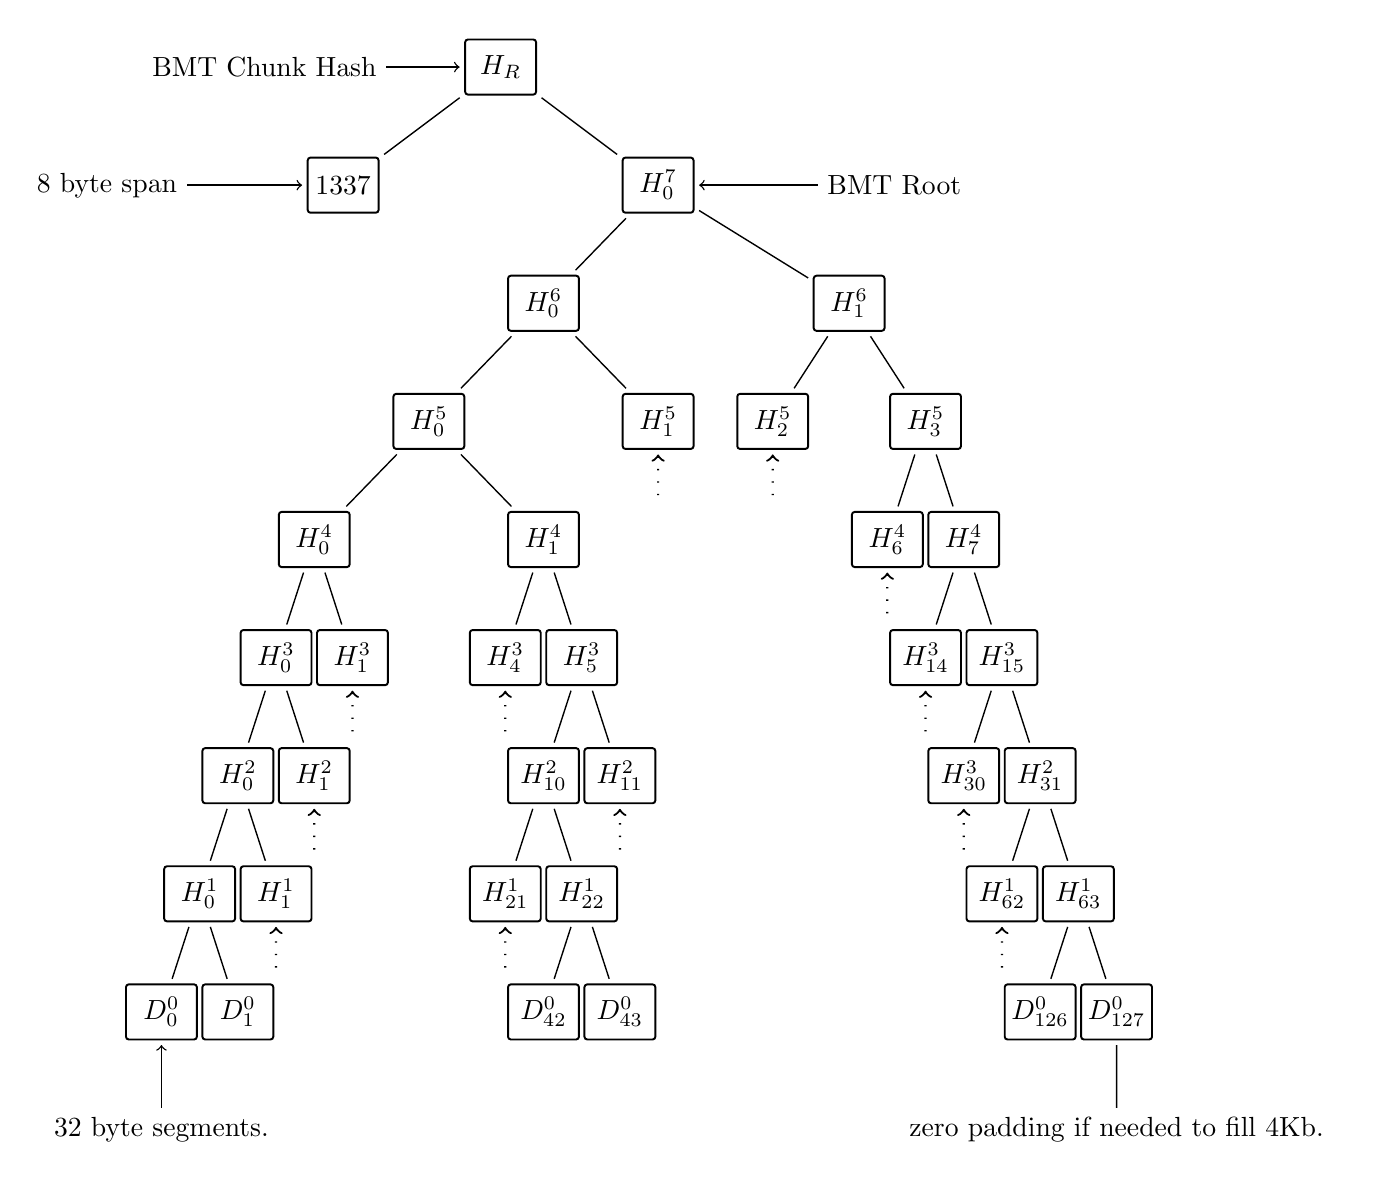
\begin{tikzpicture}
                  % level 7
\node[mtnode](bmtroot){$H_R$}
  child[<-,grow=left,level distance=3cm] { node[bubble] (ash) {BMT Chunk Hash}  }
  child[grow=down]{ node[mtnode] at (-2,0)(root) {$1337$}
    child[<-,grow=left,level distance=3cm] { node[bubble] (ash) {8 byte span}  }
  }
  child[grow=down]{ node[mtnode] at (2,0) (root) {$H^7_0$}
                  % level 6
  child[<-,grow=right,level distance=3cm] { node[bubble] (ash) {BMT Root}  }
  child { node[mppath] (6-0) {$H^6_0$}   % 0
                  % level 5
    child { node[mppath] (5-0) {$H^5_0$}          % 0
      % child[mpedge]
                  % level 4
                  % mppath goes the other way
      child { node[mpext] (4-0) {$H^4_0$}
        % % child[mtedgeadj]
                  % level 3
        child { node[mtnode] (3-0) {$H^3_0$}
              % level 2
          child { node[mtnode] (2-0) {$H^2_0$}
                % level 1
            child { node[mtnode] (1-0) {$H^1_0$}
                % level 0
              child { node[mtnode] (0-0) {$D^0_0$}
                % data level
                child[mtedge] { node[text width=3cm, align=center] (c-0) {32 byte segments.} }
              }
              % % child[mtedgeadj]
              child { node[mtnode] (0-1) {$D^0_1$}
              }
                % level 0
            }
                % level 1
            % child[mtedgeadj]
            child { node[mtnode] {$H^1_{1}$} child[ellip] }
          }
                % level 2
          % child[mtedgeadj]
          child { node[mtnode] {$H^2_{1}$} child[ellip] }
        }
                % level 3
        % child[mtedgeadj]
        child { node[mtnode] {$H^3_{1}$} child[ellip] }
      }
                % level 4
      child[missing]
      child[missing]
      child { node[mppath] (4-1) {$H^4_1$}                 % 1
                % level 3
        child { node[mpext] (3-4) {$H^3_4$} child[ellip] }
        % child[mpedge]
        child { node[mppath] (3-5) {$H^3_5$}  % 1
                % level 2
          % child[mpedge]
          child { node[mppath] (2-10) {$H^2_{10}$}           % 0
                % level 1
            child { node[mpext] (1-21) {$H^1_{21}$} child[ellip] }
            % child[mpedge]
            child { node[mppath] (1-22) {$H^1_{22}$}         % 1
                % level 0
              child { node[mppath] (0-42) {$D^0_{42}$}       % 0
              }
                % level 0
              % child[mpedge]
              child { node[mpext] (0-43) {$D^0_{43}$}
              }
                % level 0
            }
                % level 1
          }
                % level 2
          % child[mpedge]
          child { node[mpext] (2-11) {$H^2_{11}$} child[ellip] }
        }
                % level 3
        % child[missing]
      }
                % level 4
    }
                % level 5
    child[missing]
    % child[mpedge]
    child[missing]
    child { node[mpext] (5-1) {$H^5_1$} child[ellip] }
  }
                % level 6
  child[missing]
  child[missing]
  % child[mtedgeadj]
  child[missing]
  child  { node[mpext] (6-1) {$H^6_1$}
                % level 5
    child { node[mtnode] (5-2) {$H^5_2$} child[ellip] }
    child[missing]
    % child[mtedgeadj]
    child { node[mtnode] (5-3) {$H^5_3$}
                % level 4
      child { node[mtnode] {$H^4_{6}$} child[ellip] }
      % child[mtedgeadj]
      child { node[mtnode] (4-7) {$H^4_7$}
                % level 3
        child { node[mtnode] {$H^3_{14}$} child[ellip] }
        % child[mtedgeadj]
        child { node[mtnode] (3-15) {$H^3_{15}$}
                % level 2
          child { node[mtnode] {$H^3_{30}$} child[ellip] }
          % child[mtedgeadj]
          child { node[mtnode] (2-31) {$H^2_{31}$}
                % level 1
            child { node[mtnode] {$H^1_{62}$} child[ellip] }
            % child[mtedgeadj] {node {}}
            child { node[mtnode] (1-63) {$H^1_{63}$}
                % level 0
              child { node[mtnode] (0-126) {$D^0_{126}$}
              }
              % child[mtedgeadj]
              child { node[mtnode] (0-127) {$D^0_{127}$}
                child { node[draw=none, text width=6cm, align=center] (spanann) {zero padding if needed to fill 4Kb.} }
              }
                % 0
            }
                % 1
          }
                % 2
        }
                % 3
      }
                % 4
    }
               % 5
  }
}               % 6
 ;
\end{tikzpicture}
   \caption[BMT: Binary Merkle Tree hash used as chunk hash in Swarm]{BMT (Binary Merkle Tree) chunk hash in Swarm: the 1337 bytes of chunk data is segmented into 32 byte segments. Zero padding is used to fill up the rest upto 4 kilobytes. Pairs of segments are hashed together using Keccak256 to built up the binary tree. On level 7, the binary Merkle root is prepended with the 8 byte span to yield the BMT chunk hash.`}
   \label{fig:BMT}
\end{figure}

This structure  allows for compact \gloss{inclusion proofs} with a 32-byte resolution. Inclusion proof means a proof that a string is a substring of another string, for instance that a string is included in a chunk. Together with the Swarm file hash (\ref{sec:files} and \ref{spec:format:files}), it allows for logarithmic inclusion proofs for files. 

\subsubsection{Chunk encryption}\label{sec:chunk-encryption}

Content addressed chunks should be encrypted by default. Beyond client needs for confidentiality, encryption has two further important roles. (1) Obfuscation of chunk content by encryption provide a degree of \gloss{plausible deniability}; using it across the board makes this defense stronger. (2) The ability to choose arbitrary encryption keys together with the property of uniform distribution offer predictable ways of \gloss{mining chunks}, i.e., generate an encrypted variant of the same content so that the resulting chunk address satisfies certain constraints, e.g., is close to or farther away from a particular address. This is an important property used in (1) \gloss{price arbitrage} (see \ref{sec:pricing}) and (2) efficient use of postage stamps (see \ref{sec:postage-stamps}).


\begin{figure}[htbp]
   \centering
   \caption[Chunk encryption in Swarm]{Chunk encryption in Swarm}
   \label{fig:chunk-encryption}
\end{figure}


Chunk encryption (see figure \ref{fig:chunk-encryption}) is formally specified in \ref{spec:format:encryption}. Chunks shorter than 4 kilobytes are padded with random bytes (generated from the chunk encryption seed). The full chunk plain text is encrypted and decrypted using a XOR-based stream cipher seeded with the corresponding symmetric key. In order not to increase the attack surface by introducing additional cryptographic primitives, the stream cipher of choice is using 256-bit Keccak SHA3 in counter mode, i.e., hashing together the key with a counter for each consecutive segment of 32 bytes. In order to allow selective disclosure of individual segments being part of an encrypted file, yet leak no information about the rest of the file, we add an additional step of hashing to  derive the encryption key for a segment in the chunk. This scheme is easy and cheap to implement in \gloss{EVM}, lending itself to use in smart contracts constraining the plaintext of encrypted Swarm content. 

The prepended metadata encoding the chunk span is also encrypted as if it was a continuation of the chunk, i.e., with counter 128. Encrypted chunk content is hashed using the \gloss{BMT hash} just as unencrypted ones. The fact that a chunk is encrypted can be guessed from the \gloss{span value}. Apart from this, for the network layer, encrypted chunks behave exactly the same way as unencrypted ones.

\subsection{Single owner chunks}\label{sec:single-owner-chunks}

With \glossplural{single owner chunk} a user can assign arbitrary data to an address and attest chunk integrity with their digital signature. The address is calculated as the hash of an \gloss{identifier} and an \gloss{owner}. The chunk content is structured, it is composed of the identifier, the \gloss{payload} and a signature attesting to the association of identifier and payload (see figure \ref{fig:single-owner-chunks}). This structure can be described as \gloss{addressed and signed single-owner content} yielding the apt acronym \gloss{assoc}.

\begin{itemize}
    \item \emph{content}: 
\begin{itemize}
    \item \emph{identifier} - 32 bytes arbitrary identifier, 
    \item \emph{signature} - 65 bytes \emph{r,s,v}, representation of an EC signature,
    \item \emph{padding} - 23 idle bytes,
    \item \emph{span} - 8 byte chunk span,
    \item \emph{payload} - max 4096 bytes of data.
\end{itemize}
    \item \emph{address} - 256-bit keccak sha3 hash of identifier + owner public key.
\end{itemize}


\begin{figure}[htbp]
   \centering
   \caption[Assoc: addressed and signed single-owner content chunks]{Assoc: addressed and signed single-owner content chunks}
   \label{fig:single-owner-chunks}
\end{figure}

Validity of an assoc chunk is checked with the  following process:

\begin{enumerate}
    \item Deserialise chunk content into the fields for identifier, signature and payload.
    \item Construct the expected plain text composed of the identifier and the \gloss{BMT hash} of the payload.
    \item Recover the owner's address from the signature using the plain text.
    \item Check the hash of the identifier and the owner (expected address) against the chunk address.
\end{enumerate}

Assoc chunks offer a virtual partitioning of part of the address space into subspaces associated with the single owner. Checking their validity is actually an authentication verifying that the owner has write access to the address with the correct identifier (see figure \ref{fig:assoc-integrity}). 

\begin{figure}[htbp]
   \centering
%   \includegraphics{}
   \caption[Validation of assoc chunks]{Validation of assoc chunks}
   \label{fig:assoc-integrity}
\end{figure}

The notion of integrity for single-owner chunks is weaker than in the case of content addressing: After all, it is, in principle, possible to assign and sign any payload to an identifier. Nonetheless, the fact that the chunk can only be created by a single owner (of the private key that the signature requires), it is reasonable to expect uniqueness guarantees. If the owner of the private key signs two different payloads with the same identifier and uploads both chunks to Swarm, the behaviour of the network is unpredictable (see \ref{sec:feeds} for a  more detailed discussion).


\subsection{Redundancy by replication}\label{sec:redundancy-by-local-replication}

In the case of request forwarding failures, one can retry with another peer or, to guard against this, a node can start concurrent \glossplural{retrieve request} right away. Such fallback options are not available if all the \glossplural{storer node} go down. Therefore redundancy is of major importance. If the closest node is the only storer and it drops out, there is no way to retrieve the content. This basic scenario is handled by having a set of \gloss{nearest neighbours} holding replicas of each chunk that is closest to any of them. 

\subsubsection{Size of nearest neighbourhoods}

If the Kademlia connectivity is defined over storer nodes, then in a network with Kademlia topology there exists a depth $d$ such that (1) each \gloss{PO bin} less than $d$ contains at least $k$ storer peers, and (2) all \glossplural{storer node} with \gloss{PO} $d$ or higher are actually connected peers. In order to take care of redundancy, we can add to this definition a criterion that the nearest neighbourhood defined by $d$ contains at least $r$ peers.

Let us define \gloss{neighbourhood size} $\mathit{NHS}_x(d)$  as the cardinality of the neighbourhood defined by depth $d$ of node $x$. 
A node has Kademlia connectivity with redundancy factor $r$ if there exists a depth $d$ such that (1) each PO bin less than $d$ contains at least $k$ storer peers, and (2) all storer nodes with PO $d$ or higher are actually connected peers, and (3) $\mathit{NHS}_x(d)\geq r$.

Take the highest depth $d'$ such that (1) and (2) are satisfied. Such a $d$ always exists and the hive protocol can bootstrap it. As we decrease $d'$, the neighbourhoods are growing so for any redundancy parameter not greater than the network size $r\leq N=\mathit{NHS}_x(0)$, there will be a highest $0<d_r\leq d'$ such that $\mathit{NHS}_x(d_r)\geq r$. So \gloss{redundant Kademlia connectivity} is achievable. 



For a particular redundancy, the area of the fully connected neighbourhood defines an \gloss{area of responsibility}. The PO boundary of the area of responsibility defines a \gloss{radius of responsibility} for the node. A storer node is said to be \emph{responsible} for (storing) a chunk if the chunk address falls within the node's radius of responsibility. 

\subsubsection{Redundant retrievability}

A chunk is said to have \gloss{redundant retrievability} with degree $r$ if it is retrievable and would remain so after any $r$ nodes responsible for it leave the network. The naive approach presented so far requiring the single closest node to keep the content can be interpreted as degree zero retrievability. If nodes in their area of responsibility fully replicate their content (see \ref{sec:pull-syncing}), then every chunk in the Swarm DISC is redundantly retrievable with degree $r$. Let us take node $x$ that is closest to a chunk. Since it has Kademlia connectivity with redundancy $r$, there are $r+1$ nodes responsible for the chunk in a neighbourhood fully connected and replicating content. After $r$ responsible nodes drop, there is just one node remaining which still has the chunk. If Kademlia connectivity is maintained as the $r$ nodes leave, this node will be accessible from any node and therefore the chunk is still retrievable. However, for the network to ensure all chunks are redundantly retrievable with degree $r$, the new neighbourhood needs to resync their content. This is called the guarantee of \gloss{eventual consistency}.

\subsubsection{Resource constraints}

Let us assume then (1) the forwarding strategy that relays requests along \glossplural{stable node} and (2) the storage strategy that each node in the nearest neighbourhood (of $r$ storer nodes) stores all chunks the address of which fall within their radius of responsibility. As long as these assumptions hold, each chunk is retrievable even if $r$ storer nodes drop offline simultaneously. As for (2), we still need to assume that every node in the nearest neighbour set can store each chunk. Realistically, however, all nodes have resource limitations. With time, the overall amount of distinct chunks ever uploaded to Swarm will increase indefinitely. Unless the total storage capacity steadily increases, we should expect that the nodes in Swarm are able to store only a subset of chunks. Some nodes will reach the limit of their storage capacity and therefore face the decision whether to stop accepting new chunks via syncing or to make space by removing some of their chunks. 

The process that purges chunks from their local storage is called \gloss{garbage collection}. The process that dictates which chunks are chosen for garbage collection is called \gloss{garbage collection strategy} (see  \ref{spec:strategy:garbage-collection}). For a profit-maximizing node, it holds that it is always best to garbage-collect the chunks that are predicted to be least profitable in the future. Hence, in order to maximize profit, it is desired for a node to get this prediction right (see \ref{sec:postage-stamps}). In order to factor in capacity constraints, we will introduce the notion of \gloss{chunk value} and modify the definitions using the minimum value constraint:

In Swarm's DISC, at all times there is a chunk value $v$ such that every chunk with value greater than $v$ is retrievable and eventually (after syncing) redundantly retrievable with degree $r$ .

% \subsection{}\label{sec:}

\section{Push and pull: chunk retrieval and syncing}\label{sec:push-and-pull}
\green{}
In this section, we demonstrate how chunks actually move around in the network: How they are pushed to the storer nodes in the neighbourhood they belong when they are uploaded as well as how they are pulled from the storer nodes when they are downloaded.

\subsection{Retrieval}\label{sec:retrieval}

In a distributed chunk store, we say that a chunk is \emph{accessible} if a message is routable between the requester and the node who stores the chunk. Assuming that the node closest to the chunk address actually stores the chunk, sending a retrieve request message to the chunk address will reach the storer node. In a distributed chunk store with healthy Kademlia topology all chunks are accessible for every node.

\subsubsection{Chunk delivery}

For retrieval, accessibility needs to be complemented with a process to have the content delivered back to the requesting node preferably using the chunk address only. There are at least three alternative ways to achieve this (see figure \ref{fig:chunk-delivery}):

\begin{enumerate}
    \item \gloss{direct delivery} - The chunk delivery is sent via a direct underlay connection. 
    \item \gloss{routed delivery} - The chunk delivery is sent as message using routing.
    \item \gloss{pass-back delivery} - The chunk delivery response simply follows the request route back to the originator.
\end{enumerate}


\begin{figure}[htbp]
   \centering
%   \includegraphics{}
   \caption[Alternative ways to deliver chunks: direct, routed and pass-back]{Alternative ways to deliver chunks: direct, routed and pass-back}
   \label{fig:chunk-delivery}
\end{figure}

Direct delivery means that chunk delivery happens in one step via some lower level network protocol. This would require an adhoc connection with latency trading off for security. Either direct or routed, allowing deliveries routed independently of the request route presupposes that the requestor's address is (at least partially) known, i.e., it leaks identity information on the requestor. With forwarding Kademlia and pass-back delivery this is not necessary: The storer node just responds back to their requesting peer with the delivery, while intermediate forwarding nodes remember which of their peers requested which chunk and when the delivery arrives they just pass it back to their immediate requestors. In other words, the chunk delivery response simply follows the request route back to the originator (see figure \ref{fig:request-response}). This makes it possible to not disclose requestor identity in any form, and thus implements \gloss{anonymous retrieval}. 

\begin{figure}[htbp]
   \centering
%   \includegraphics{}
   \caption[Pass-back: pattern for anonymous request-response roundtrips in forwarding Kademlia]{Pass-back: pattern for anonymous request-response roundtrips in forwarding Kademlia.}
   \label{fig:request-response}
\end{figure}

Requestor anonymity by default in the retrieval protocol is a crucial feature that Swarm offers for privacy and censorship-resistant access, therefore we do not pursue alternatives here.%
%
\footnote{Beeline delivery has some merit, i.e., bandwidth saving and better latency, we do not completely rule out the possibility of implementing it. 
}


This generic solution has further benefits relating to spam protection, scaling and incentivisation discussed in the remainder of this section.

\subsubsection{Protection against unsolicited chunks}

In order to remember requests, the forwarding node needs to create a resource which bears some cost (takes space in memory). The requests that are not followed by delivery should eventually be garbage collected, so there needs to be a time period while they are active. Downstream peers need to be informed about the timeout of the request. This makes more sense since the originator of the request want to attach a time to live duration to the request.  

Sending unsolicited chunks is an offence as it can lead to DDOS. By remembering the request, nodes can recognise unsolicited chunk deliveries and penalise peers sending them. Chunks that are delivered after the request expires will be treated as unsolicited. Since there may be some discrepancy assessing the expiry time between nodes, there needs to be some tolerance for unsolicited chunk deliveries, but it they go above a particular (still small) percentage of requests forwarded, the offending peer is disconnected and blacklisted. Such local sanctions are the easiest and simplest way to incentivise adherence to the protocol (see \ref{sec:sanctions}). 

\subsubsection{Rerequesting}

Potentially, a large proportion of Swarm nodes are not stably online. Such a high churn situation is problematic if we use the naive strategy of forwarding requests to any one closer node. If a node on the path goes offline before delivery, then the request--response roundtrip is broken, effectively rendering the chunk requested not retrievable. Commitment to pay for a chunk is considered void if the requested peer is dropped so there is no harm in rerequesting the chunk from another node (see \ref{spec:strategy:forwarding}).


\subsubsection{Timeout vs not found}

Note that in Swarm there is no explicit negative response for chunks not found. In principle, the node that is closest to the retrieved address can tell that there is no chunk at this address and could issue a "not found" response, however this is not desirable for the following reasoning: While the closest node to a chunk can verify that a chunk is indeed not at the place in the network where it is supposed to be, all nodes further away from the chunk cannot credibly conclude this as they cannot verify it first-hand and all positive evidence about the chunk's retrievability obtained later is retrospectively plausibly deniable. 

All in all, as long as delivery earns more for the storer, the strategy is to keep a request open until it times out and be prepared for the chunk to appear. There are several ways the chunk can arrive after the request: (1) syncing from peers (2) appearance of a new node or (3) if a request precedes upload, e.g., requestor "subscribes" to a single-owner address (see \ref{sec:messaging}) to  decrease latency of lookup. This is conceptually different from server-based architectures where it makes sense to expect a resource to be either on the host server or not. 
 

\subsubsection{Opportunistic caching}

Using the pass-back mechanism for request-delivery also enables \gloss{opportunistic caching}, i.e., when a forwarding node receives a chunk, then the chunk is saved in case it will be requested again. This mechanism is crucial in making Swarm scale storage of popular content automatically (see \ref{sec:caching}).

\subsubsection{Conclusion}

So far, we have shown that using the retrieval protocol and maintaining Kademlia connectivity, nodes in the network are capable of retrieving chunks. However, since forwarding is using a scarce resource (bandwidth), without accounting, network reliability will be contingent on the proportion of freeriding and altruism. Instead, in section \ref{sec:incentivisation}, we provide a system of economic incentives that align with desired behaviour. In other words, profit maximising strategies by node operators adhering to the protocol give rise to emergent behaviour that is beneficial for users of the network as a whole.
 
\subsection{Push syncing}\label{sec:push-syncing}
 
In the previous sections, we presented how a network of nodes maintaining a Kademlia overlay topology can be used as a distributed chunk store and how forwarding Kademlia routing can be used to define a  protocol for retrieving chunks.
Retrieval assumed that chunks are located with the node whose address is closest to theirs. This section describes the protocol responsible for realising this assumption: delivering the chunk to its storer after it is uploaded to an arbitrary node.

This network protocol, called \gloss{push syncing}, is analogous to chunk retrieval: A chunk is relayed via the same route as a retrieval request would be to reach the node closest to the chunk address, and, in response, a \gloss{statement of custody receipt} is passed back along the same path (see figure \ref{fig:push-syncing}). The statement of custody sent back by the storer to the \gloss{uploader} is meant to indicate that the chunk has reached the neighbourhood where it is universally retrievable from. By tracking these responses for each chunk constituting an upload, uploaders can make sure that their upload is fully retrievable before sharing/publishing their upload. Keeping a count of chunks push-synced and receipts received serves as the backend for a \emph{progress bar} that can be shown to the uploader as part of the user experience (see \ref{sec:upload} and \ref{spec:api:tags}).


\begin{figure}[htbp]
   \centering
%   \includegraphics{}
   \caption[Push syncing]{Push syncing}
   \label{fig:push-syncing}
\end{figure}

Statements of custody are signed by the nodes that claim to be the closest to the address.%
%
\footnote{As long as there is no way to verify  which node is actually closest to the chunk, it is possible to conduct a grieving attack where a malicious node would eclipse the route for some chunks and respond with statements of custody while not actually forwarding the message which would result in the publisher falsely assuming their upload to be retrievable. This is best mitigated by having pull syncing (\ref{sec:pull-syncing}) in place which channels the chunks to every peer closer and is much harder to attack. Alternatively nodes could be punished with a fingerpointing mechanism but that requires stake and registration.}
%
Similarly to downloaders in the retrieval protocol, the identity of uploaders can also remain hidden, hence forwarding Kademlia can implement \gloss{anonymous uploads}.

Another similarity is that in order to allow the pass-back mechanism for responses, nodes should remember which peer sent a particular chunk. This record should persist for a short period while the statement of custody responses are expected. When this period ends, the record is removed. A statement of custody not matching a record is considered unsolicited and is allowed only up to a small percentage of all push-sync traffic with a peer. Going above this tolerance threshold is sanctioned with disconnection and blacklisting (see \ref{sec:sanctions}).

In this section we described how the logistics of chunk uploads can be organised with a network protocol using forwarding Kademlia routing with response back-passing. This solution is only complete once it is secured with aligned incentives: The strategy to follow this protocol should be incentivised and DDOS abuse should be disincentivised. These are discussed in detail in \ref{sec:postage-stamps} and TODO<>REFERENCE to new Push sync incentives chapter.

\subsection{Pull syncing}\label{sec:pull-syncing}

\glossupper{pull syncing} is the protocol that is responsible for 

\begin{itemize}
    \item \emph{eventual consistency} - Syncing neighbourhoods as and when the topology changes due to churn or new nodes joining.
    \item \emph{maximum resource utilisation} - Nodes can pull chunks from their peers to fill up their surplus storage. 
    \item \emph{fallback push mechanism} - If push syncing is not available, pull syncing can cover this functionality.  
\end{itemize}

Pull syncing is node centric as opposed to chunk centric, i.e., it makes sure that a node's storage is filled if needed as well as syncing chunks in a neighbourhood. When two nodes are connected they will start syncing both ways. On each peer connection there is bidirectional chunk traffic. The two directions of syncing are managed by distinct and independent \emph{streams} (see \ref{spec:protocol:stream}). In the context of a stream, the consumer of the stream is called \gloss{downstream peer} or client, while the provider is called the \gloss{upstream peer} or server. 

When two nodes connect and they engage in \gloss{chunk synchronisation}, the upstream peer offers all the chunks it stores locally in a data stream per proximity order bin. To receive chunks closer to a downstream than to the upstream, downstream peer can subscribe to the chunk stream of the PO bin that the upstream peer belongs to in their Kademlia table. If the peer connection is within the nearest neighbour depth $d$, the client subscribes to all streams with PO bin $d$ or greater. As a result, peers eventually replicate all chunks belonging to their area of responsibility.

Pull syncing server behaviour is defined as a \gloss{stream provider} (\ref{spec:protocol:pull-sync}) using the stream protocol (see \ref{spec:protocol:stream}). Nodes keep track of when they stored a chunk locally (by indexing them by an ever increasing storage count, called \gloss{bin ID}). For each PO bin, upstream peers offer to stream chunks in order of storage timestamp. As a result of syncing streams on each peer connection, a chunk can and would be synced to a downstream peer from multiple upstream peers. In order to save bandwidth by not sending chunk data over to peers that already have them, the stream protocol implements a roundtrip: Before sending chunks, upstream peer offers a batch of chunks identified by their address, to which downstream responds with stating which chunks in the offered batch they actually need (see figure \ref{fig:pull-syncing}). Note that this critically relies on the chunk integrity assumption discussed in \ref{sec:chunks}.


\begin{figure}[htbp]
   \centering
%   \includegraphics{}
   \caption[Pull syncing]{Pull syncing}
   \label{fig:pull-syncing}
\end{figure}

In the context of a peer connection, client is said to be \emph{synced} if it has synced all the chunks of the upstream peer. Note that due to disk capacity limitations, nodes must impose a value cutoff and "all chunks" reads as "all chunks having value greater than $v$". In  order for a node to promise they store all chunks with value greater than $v$, all its neighbours must have stored all chunks greater than value $v$. In other words, nodes syncing inherit the maximum such value among their storer peers. 

If chunks are synced in order of storage this may not result in the node having the most profitable (most often requested) chunks. Thus it may be advisable to sync chunks starting with the most popular ones according to upstream peers and finish syncing when storage capacity is reached. This way, a node's limited storage will be optimised. Syncing and garbage collection are discussed further in \ref{sec:postage-stamps} and \ref{sec:capacity-pressure} and a consolidated client strategy is specified in \ref{spec:strategy:pull-sync}.

To conclude this section, we show how the criteria of \gloss{eventual consistency} are met in a healthy Swarm. Chunks found in local store of any node will become retrievable after being synced to their storers. This is because as peers pull chunks closer to  them than to the upstream peer, each chunk travels routes that would qualify as valid forwarding paths in the push sync protocol. If new nodes are added, and old nodes drop out, neighbourhoods change, but as long as local redundancy is high enough that churn can not render previously retrievable chunks non-retrievable, neighbourhoods eventually replicate their content and redundancy is restored. 


\subsection{Light nodes}
\label{sec:light}

The concept of \gloss{light node} refers to a special mode of operation necessitated by poor bandwidth environments, e.g., mobile devices on low throughput networks or devices allowing only transient or low-volume storage.

A node is said to be light by virtue of not participating fully in the usual protocols detailed in the previous sections, i.e., retrieval, push syncing or pull syncing. 

A node that has restricted bandwidth environment or in whatever way has limited capacity  to maintain underlay connections is not expected to be able to forward messages conforming to rules of Kademlia routing. This needs to be communicated to its peers so that they do not relay messages to it. 

As all protocols in Swarm are modular, a node may switch on or off any protocol independently (depending on capacity and earnings requirements). To give an example: a node that has no storage space available, but has bandwidth, may participate as a forwarding node only. Of course, while switching off protocols is technically feasible, a node must at all times take into account that his/her peers expect a certain level of service if this is advertised and may not accept that some services are switched off (at the risk of blacklisting). 

----Proposing to delete START

Since forwarding can earn revenue, these nodes may still be incentivised to accept retrieve requests. However, if the light node has Kademlia connectivity above PO bin $p$ (i.e., they  are connected to all storer nodes within their nearest neighbourhood of $r$ peers at depth   $d$, and there is at least one peer in each of their PO bin from $p$ to $d$), they can advertise this and participate in forwarding. 

When they want to retrieve or push chunks, if the chunk address falls into a PO bin where there are no peers, they just pick a saturated peer in another bin. Though this may result in a spurious hop (when the proximity of the message  destination to the latest peer does not increase as a result of the relaying), the Kademlia assumption that routing can be completed in logarithmic steps still holds valid.

A node that is advertised as a storer/caching node is expected to store all chunks  above a certain value. In order to have consistency, they need to syncronise content in their area of responsibility which necessitates running the pull sync protocol. This is so also with aspiring storer nodes, which come online with available storage and open up to pull-sync streams to fill their storage capacity. In the early stages of this, it does not make sense for a node to sync to other full storer nodes. However, they can still be useful to sync to other similar newcomer nodes, especially if storer nodes are maxing out on their bandwidth.

The crucial thing here is that for redundancy and hops to work, light nodes with   incomplete, unsaturated Kademlia tables should not be counted by other peers towards saturation.

----Proposing to delete END

\chapter{Incentivisation}\label{sec:incentivisation}
The Swarm network comprises independent nodes, running software which implements the Swarm protocol (see: \ref{spec:protocol}). It is important to realize that, even though nodes run the same protocol, the emergent behavior of the network is not guaranteed by the protocol alone; as nodes are autonomous, they are essentially "free" to react in any way they desire to incoming messages of peers.
It is, however possible to make it profitable for a node to react in a way that is beneficial for the desired emergent behavior of the network, while making it costly to act in a way that is detrimental. Broadly speaking, this is achieved in Swarm by enabling a transfer of value from those nodes who are using the resources of the network (\glossplural{net user}) to those who are providing it (\glossplural{net provider}). 
The rest of this chapter is concerned with describing the desired emergent behaviour of the network (\ref{sec:emergent_behavior}), after which we describe the actions which incur costs and those that provide value (\ref{sec:cost_benefit}). Finally, we proceed by describing the incentive mechanisms which ensures that costs are borne as directly as possible by the initiator of the action, with benefits flowing to the nodes who provided the initiator with the expected outcome, ultimately facilitating the desired emergent behavior (see \ref{sec:incentive_mechanisms}).

\section{Incentive design}
\wip{foundational requirement + analysis} 
\subsection{WIP Desired emergent behavior}\label{sec:emergent_behavior}
\subsection{WIP Analysis on expected costs and benefits of actions}\label{sec:cost_benefit}
\subsection{WIP Proposed incentive mechanisms}\label{sec:incentive_mechanisms}
This section will constitute most of the sections which are already described below.


\section{Sharing bandwidth}

\green{}

\subsection{Incentives for serving and relaying}\label{sec:incentives-relaying}

\green{}

\subsubsection{Forwarding Kademlia and repeated dealings}

Retrieval of a chunk is ultimately initiated by someone accessing content and therefore, all costs related to this retrieval should be borne by them. While paid retrievals may not sound like a popular idea when today's web is "free", many of the problems with the current web originates precisely from the fact that consumers are not able to share the costs with content publishers directly. In principle, the retrieval of a chunk is a functional unit where storer acts as service provider and requestor as consumer. As service is given by provider to consumer, compensation should be given by consumer to provider. Such a direct transaction would require that transactors are known to each other, so if we are to maintain the anonymity requirement on  downloads, we need to conceptualise compensations in a different way. 

If we use forwarding Kademlia, chunk retrieval subsumes a series of relaying actions performed by forwarding nodes. Since these are independent actors, it is already necessary to incentivise each act of relaying. Importantly, if only instances of relaying are what matters, then, irrespective of the details of accounting and compensation (see \ref{sec:accounting}), transactors are restricted to connected peers. Given the set of ever connected peers is a quasi-permanent set across sessions, this allows us to frame the interaction in the context of \gloss{repeated dealings}. Such a setting always creates extra incentive for the parties involved to play nice. It is reasonable to exercise preference for peers showing untainted historical record. 

Moreover, since the quasi-permanent set is logarithmic to network size, any book-keeping or blockchain contract that the repeated interaction with a peer might necessitate is kept manageable, offering a scalable solution.

\subsubsection{Charging for pass-back response}

If accepting a retrieve request already constitutes revenue for forwarding nodes (in the sense of triggering an accounting event before the response delivered), then it creates a perverse incentive not to forward. Conditioning the request revenue on successful retrieval is a potential solution: The accounting event is triggered when a requested chunk is delivered.

If, however, there is no cost to a request then spamming with requests for non-existing chunks (random addresses) becomes possible. This can be mitigated by simply disconnecting from peers that send too many requests for chunks that do not exist. Note that policing requestors is much easier than policing forwarders, since the latter requires positive evidence from other nodes while the former only requires forwarding: In practice then, a node keeps a record of the request of its peers and updates the relative frequency of failed requests (requests that time out); if the percentage of these relative to all requests is too high, the peer is sanctioned with disconnection and blacklisting (see \ref{sec:sanctions}).

Once a node forwards a request, it commits to pay for the chunk if and when delivered within the \gloss{TTL}, therefore there is never an incentive to block timely deliveries when the chunk is passed back.  This commitment also prevents nodes from just frivolously asking several peers for a chunk, since, if  multiple peers respond with delivery, they all need to be paid.


\subsection{Pricing protocol for chunk retrieval}\label{sec:pricing}

\green{}

We describe a protocol which nodes use to communicate their price for delivering chunks in the Swarm network. On top of this protocol, strategies can be implemented by nodes who wish to compete with other nodes on quality/price. 

\subsubsection{Price discovery}\label{sec:retrieval-price-discovery}

The price signalling is closely coupled with actual retrieve requests and therefore is formulated as part of the retrieval protocol (see \ref{spec:protocol:retrieval}). The main merit of the protocol is that it allows for price discovery on local decisions, which is essential for the following reasons: (1) Bandwidth costs are not homogeneous around the world. Allowing nodes to express their cost structure via their price will enable competition on price and quality, ultimately benefiting the end-user. (2) The demand for bandwidth resource is constantly changing due to changes in usage or connectivity. Being able to react directly to changes creates a self-regulating system. Practically, without this possibility, a node operator might decide to shut down their node when costs go up or conversely end-users might overpay for an extended period of time when costs or demand decrease and there is no competitive pressure for nodes to reduce their price accordingly. 

In general, we believe that bandwidth is a service that comes with "instant gratification" therefore immediate acknowledgement and accounting of its cost is justified. Also, since it is hard to think of any externality or non-linearity in their overall demand and supply, a pricing mechanism which provides for both efficient and immediate signalling as well as competitive choice with minimal switching or discovery cost is likely to accommodate strategies that result in a globally optimal resource allocation.

We introduce into the retrieval protocol a message that can communicate the prices to upstream peers (see \ref{spec:protocol:retrieval}. We can conceptualise this message as an alternative response to a request. Nodes maintain the prices associated with each peer so when they issue a retrieve request they know the price they commit to pay in the event of downstream peer delivers the valid chunk within the time to live period. However, there is no point in restricting the price signal to responses: For whatever reason a peer decides to change the prices, it is in the interest of both parties to exchange this information. Even if there is nothing to respond to. Surely, in order to prevent DDOS attacks by flooding upstream peers with price change messages, the rate of price messages is limited to a small finite number between any two requests.%
%
\footnote{If a peer sets their price too high or their prices exhibit a much higher volatility than others in the network, their peers will be less likely to request chunks from them. While this suggests that unreasonable pricing is taken care of by market forces, in order to prevent catastrophic connectivity changes as a result of radical price fluctuations, limiting the rate of change may need to be enforced on the protocol level.}

For simplicity of reasoning we posit that the default price is zero, corresponding to a free service (altruistic strategy, see \ref{spec:strategy:pricing}). 

\subsubsection{Differential pricing of proximities}\label{sec:diff-pricing-prox}

If the price of a chunk is the same at all proximities, then there is no real incentive for nodes to forward requests other than the potential to cache the chunk and earn revenue by reselling it. This option is hard to justify for new chunks, especially if they are in the shallow proximity orders where they are unlikely to be requested. More importantly, if pricing of chunks is uniform across proximity orders, colluding nodes can generate chunk traffic and pocket exactly as much as they send, virtually a free DDOS attack (see figure \ref{fig:ddos-uniform-price}).

\begin{figure}[htbp]
   \centering
%   \includegraphics{}
   \caption[Uniform chunk price across proximities allows a ddos]{Uniform chunk price across proximities allows a ddos}
   \label{fig:ddos-uniform-price}
\end{figure}

To mitigate this attack the price a requestor pays for a chunk needs to be strictly greater than what the storer node receives as compensation when a request is routed from requestor to storer. We need to have a pricing scheme that rewards forwarding nodes, hence necessitates the need for differential pricing for retrieval requests for proximities. If the price of delivery is lower for any node that is further from the chunk, then the request can always be sent that way. This means that any differential scheme will converge to a pricing where delivery costs more if the peer is further from the chunk address, i.e., rewards for chunk deliveries are a decreasing function of proximity. 

It is reasonable to model pricing based on the cost of forwarding which is expected to be uniform along the delivery path. This means that the differential a node is adding to the downstream price is constant, and the overall price of chunk deliveries has a component that is a linearly decreasing function of the proximity of the originating node and the chunk address ($p$). With this information, we can express the price function for chunk delivery as $s-fp$, where $f$ is the forwarding price per hop and $s$ the price charged by the storer node. Due to competitive pressure along the delivery path and in the neighborhood, we expect both $f$ and $s$ to converge towards the marginal cost for the network to deliver the chunk.

\subsubsection{Uniformity of price across peers}

Imagine a forwarding node needs to forward a request for a chunk whose proximity order is $p$ with respect to the node. 
Peers in bin $p$ have proximity greater than $p$ to the chunk. Let's consider the peers that are closest to the chunk with PO $p+r$. If their minimum price for chunks in bin $p+r$ is greater than peers with PO $p+r-1$, then we choose a node from the latter set, see figure  \ref{fig:price-arbitrage}. This will direct traffic away from the costlier region and increase traffic in the cheaper region. As a consequence prices will adjust. 

\begin{figure}[htbp]
   \centering
   \caption[??? Price arbitrage]{??? Price arbitrage}
   \label{fig:price-arbitrage}
\end{figure}

Let us assume the cheapest price for our chunk is given by the nearest peers having PO $p+1$ from the chunk (this can happen if there is only a single connected peer in the nodes $p$ bin or if the peers are not  balanced. By definition, the peers that are closer than $p$ have the same proximity $p$ to the chunk. This means that as long as any peer closer to the node than $p$ offers a lower price than the node itself for chunks of PO $p$, the request can just be forwarded to that node making a profit on the price difference. Note that this is not ideal for the network as it introduces a \gloss{spurious hop} in routing, i.e., in relaying without increasing the proximity. However, it has the consequence that even if peers in a bin are colluding to raise their price for PO $p+1$ they cannot raise it above the cheapest peers price for PO $p$, see figure  \ref{fig:price-arbitrage}; if they do, again, traffic will be redirected and the changing demand regulates the price back to normal. 

All else being equal, this price arbitrage strategy will achieve (1) uniform prices for the same proximity order across the network, (2) prices that linearly decrease as a function of proximity (3) nodes can increase connectivity and keep prices lower.


\subsubsection{Bin density}

Charging based on the downstream peer's proximity to the chunk has the important consequence that the net revenue earned from a single act of non-local delivery to a single requestor is a monotonically increasing function of the difference between the chunk's proximity to the node itself vs to the peer the request was forwarded to. In other words, the more distance we can cover in one forward request, the more we earn. This incentive aligns with downloader's interest to save hops in serving their requests leading to lower latency delivery and less bandwidth overhead. This scheme incentivises nodes to keep a gap-free balanced set of addresses in their Kademlia bins as deep as possible (see figure \ref{fig:densebins}), i.e, dense Kademlia bins vs thin ones.

\begin{figure}[htbp]
   \centering
%   \includegraphics{}
   \caption[Dense Kademlia bins]{Dense Kademlia bins}
   \label{fig:densebins}
\end{figure}


Nodes that are able to maintain denser bins actually have the same cost as thinner ones. But saving hops will improve latency and make the peer more efficient. This may lead to the peer being preferred to other peers that with the same prices. Increased traffic essentially can lead to bandwidth contention which eventually necessitates raising prices. 

\begin{figure}[htbp]
   \centering
%   \includegraphics{}
   \caption[Price arbitrage]{Price arbitrage}
   \label{fig:pricearbitrage}
\end{figure}

Note that such arbitrage is more efficient in shallower bins where the number of peers to choose from is higher. This is in major opposition to deep bins in the area of responsibility. If a node does not replicate its neighbourhoods chunks, some of these chunks will need to be requested by the node closer to the address but further from the node. This will only be possible at a loss. Another incentive for neighbours to replicate their area of responsibility is discussed in \ref{sec:postage-lottery}. With the area of responsibility stored however, a node can set their price arbitrarily. 


\subsubsection{Caching and auto-scaling}\label{sec:caching}

Nodes receive a reward every time they serve a chunk, therefore the profitability of a chunk is proportional to its popularity: the more often a chunk is requested, the higher the reward relative to the fixed cost of storage per time unit. When nodes reach storage capacity limits and it comes to deciding which chunks to delete, the optimal strategy of a rational profit maximising agent is to remove chunks whose profitability is lowest. A reasonably good predictor for this is the age of last request. In order to maximise the set of chunks to select from, nodes engage in opportunistic caching of the deliveries they relay as well as the chunks they sync. This results in popular chunks being more widely spread and faster served, effectively making the entire Swarm an auto-scaling and auto-balancing content distribution network.%
%
\footnote{Better metrics for predicting chunk profitability than the age of last request are expected to be identified and developed by a storer nodes (see \ref{spec:strategy:garbage-collection})}.

% Typically a chunk will be worth storing in bin $i$ needs to be twice as popular as a chunk that is worth having in bin $i+1$.

\subsubsection{Non-caching nodes}

Any scheme which leaves \glossplural{relaying node} a profit creates a positive incentive for forwarding-only non-caching nodes to enter the network. Such nodes are not inherently beneficial to the network as they are creating unnecessary bandwidth overhead. On the one hand, their presence could in principle unburden storer nodes from relaying traffic, so using them in shallow bins may not be detrimental. On the other hand, closer to neighbourhood depth, their peers will favour a caching/storing node to them because of their disadvantage at least for chunks in their hypothetical area of responsibility. Non-caching nodes can also contribute to increase anonymity (see \ref{sec:retrieval}).

\subsection{Incentivising push-syncing}\label{sec:push-sync-incentives}

\green{}

Push-syncing (see \ref{sec:push-syncing}) is the protocol by which chunks are uploaded into the network. In what follows, we explain how forwarding is incentivised.%
%
\footnote{To complement our solution for bandwidth compensation, further measures are needed for spam protection and storage incentivisation which are discussed in \ref{sec:postage-stamps} and \ref{sec:postage-lottery}, respectively}

The push sync protocol is analogous to 
the retrieval protocol in that their respective message exchange sequences travel the same route.
The delivery of the chunk in the push sync protocol is analogous to a retrieve request whereas the statement of custody receipt in push sync is analogous to the chunk delivery response in retrieval. On the analogy of the retrieval  protocol, only the statement of custody  pass-back responses will trigger an accounting event.

Requiring payment for push-sync delivery by the downstream peers would put the forwarder in a position to bargain with a storer node on the delivery of the chunk. The possession of a chunk is valuable for the prospective storer node (given that there is a system of rewards  for storage, see \ref{sec:postage-lottery}) the forwarder node could in theory hold onto the chunk unless the storer node pays marginally more than what the possession of this chunk is worth for them. Especially, since forwarders on route from the uploader are not numerous, any profit coming from a reward mechanism for storage could be captured by the forwarding nodes.

However,  making only the statement of custody receipt a paid message, roles switch. Now, a forwarder node is not in the position to bargain. To see why, consider what would happen if a forwarded node tries to hold onto a chunk to get a price for pushing this chunk to a storer node: the uploader will not get a statement of custody receipt in due time and will re-upload the chunk via a different route. Now, the original forwarding node suddenly has to compete with another forwarding node in getting compensation for their bandwidth costs. Since all forwarding nodes know that, eventually, there will be a series of peers that are willing to forward the chunk to the storer node for a small compensation for only the bandwidth costs incurred. Therefore there is no point for the original forwarding node to try and bargain with the storer node in the first place since they can make that small  profit right when they pass back the statement of custody receipt.

\begin{figure}[htbp]
\centering
\caption[Incentives for push-sync protocol]{Incentives for push-sync protocol}
\label{fig:syncing-swap}
\end{figure}

This scheme makes it clear why the incentivisation of the two  protocols relies on the same premises: there are many sellers (forwarders) and only one buyer (uploader) for a homogeneous good (the statement of custody receipt). This drives the price of the service (delivering the chunk to the storer) to the sum of all marginal cost of forwarding for each node along the route, while simultaneously allowing the storer node to capture all profits from the storage compensation scheme.

This way we can make sure that (1) storers actually respond with receipts, and (2) have a way to detect timed out or unsolicited receipt responses to protect against DoS, see figure \ref{fig:syncing-swap}.

Just as in the retrieval protocol, the pricing is expected to be different for different proximities (see \ref{sec:diff-pricing-prox} and as the costs of the nodes in the network change (depending on capacity utilization and efficiency of nodes), the pricing will be variable over time as well. Since at the point of accounting the compensation is due for one chunk and one shorter message (retrieve request and custody receipt), we can safely conclude that the price structure for forwarding in the case of the two protocols are identical and therefore one generic forwarding pricing scheme can be used (see  \ref{sec:retrieval-price-discovery}) 
 

\section{Swap: accounting and settlement}\label{sec:accounting-and-settlement}

\green{}

This section covers aspects of incentivisation relating to bandwidth sharing. 
In \ref{sec:accounting}, we introduce a mechanism  to keep track data traffic between  peers and offers peer to peer accounting for message relaying.
Subsequently, in  \ref{sec:cheques}, we describe the conditions of compensating for unbalanced services and show how settlement can be achieved.
In particular we introduce cheques and the chequebook contract. In \ref{sec:waiver}, we discuss waivers, a further optimisation allowing for more savings on transaction cost. In \ref{sec:zero-cash-entry} we discuss how an incentivised service of sending in cashing transactions enables zero-cash entry to Swarm.
Finally, in \ref{sec:sanctions} discusses basic sanctions that serve as fundamental incentive to play nice and adhere to protocols.

\subsection{Peer to peer accounting}\label{sec:accounting}


\cite{ethersphere2016sw3} introduces a protocol for peer-to-peer accounting, called \gloss{swap}. swap is a tit-for-tat accounting scheme that scales microtransactions (see \ref{spec:protocol:swap}). The scheme allows directly connected peers to swap payments or payment commitments. The major features of the system are captured playfully with different mnemonic resolutions of the acronym swap:

\begin{itemize}
    \item \emph{Swarm accounting protocol} for \emph{service wanted and provided} -- Account service for service exchange.
    \item \emph{settle with automated payments} -- Send \gloss{cheque} when payment threshold is exceeded.
    \item \emph{send waiver as payment} -- Debt can be waived in the value of uncashed cheques. 
    \item \emph{start without a penny} and \emph{setup wallet as payment} -- Zero cash entry is supported by unidirectional swap.
\end{itemize}

\subsubsection{Service for service}

Swap allows service for service exchange between connected peers (\emph{swap = Swarm accounting protocol for service wanted and provided}). In case of equal consumption with low variance over time, bidirectional services can be accounted for without any payments. Data relaying is an example of such a service, making swap ideally suited for implementing bandwidth incentives in content delivery or mesh networks.

\begin{center}
\begin{figure}[htbp]

\begin{center}
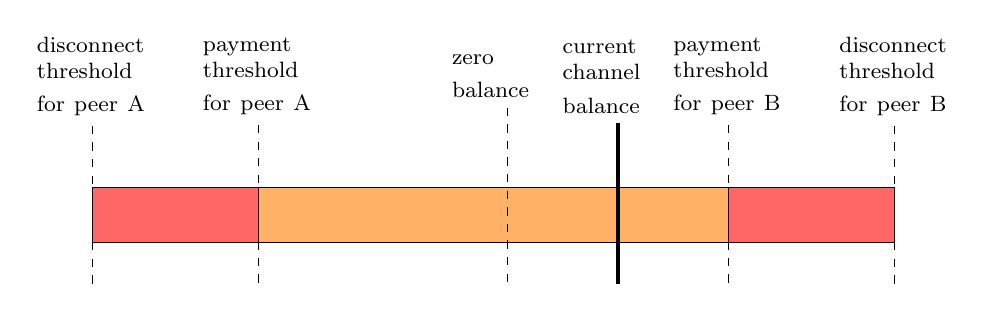
\begin{tikzpicture}
\node (middle)[draw, rectangle, fill=orange!60, minimum height=2em, minimum width=18em]{};
\node (leftred) [draw, rectangle, fill=red!60, minimum height=2em, minimum width=6em, node distance=12em,left of=middle]{};
\node (rightred)[draw, rectangle, fill=red!60, minimum height=2em, minimum width=6em, node distance=11em,right of=middle]{};
\node (zero) [above of=middle,node distance=5em, text width=4em, align=left] {\footnotesize zero\\ balance};
\node (zerod) [below of=middle] {};
\draw [dashed](zero)--(zerod);
\node (rtol) [node distance=8em,right of=zero,text width=4em, align=left] {\footnotesize payment\\threshold\\for peer B};
\node (rtold) [node distance=8em,right of=zerod] {};
\node (ltol) [node distance=9em,left of=zero,text width=4em, align=left] {\footnotesize payment\\threshold\\for peer A};
\node (ltold) [node distance=9em,left of=zerod] {};
\node (rdis) [node distance=14em, right of=zero,text width=4em, align=left] {\footnotesize disconnect\\threshold\\for peer B};
\node (rdisd) [node distance=14em,right of=zerod] {};
\node (ldis) [node distance=15em, left of=zero,text width=4em, align=left] {\footnotesize disconnect\\threshold\\for peer A};
\node (ldisd) [node distance=15em,left of=zerod] {};
\node (rbal) [node distance=4em,right of=zero,text width=4em, align=left] {\footnotesize current\\channel\\balance};
\node (rbald) [node distance=4em,right of=zerod] {};

\draw [dashed](rtol)--(rtold);
\draw [dashed](ltol)--(ltold);
\draw [dashed](rdis)--(rdisd);
\draw [dashed](ldis)--(ldisd);
\draw [very thick](rbal)--(rbald);
\end{tikzpicture}
\end{center}
\caption[Swap balance and swap thresholds]{Swap balance and swap thresholds.
Zero balance in the middle indicates consumption and provision are equal.
The current channel balance represents the difference in uncompensated service provision:
If to the right of zero, the balance tilts in favour of A with peer B being in debt, whereas to the left
the balance tilts in favour of B with A being in debt.
The orange interval represents loss tolerance. If the balance goes over the payment threshold, the party in
debt sends a cheque to its peer, if it reaches the disconnect threshold, the peer in debt is disconnected.}
\label{fig:swap}
\end{figure}
\end{center}

\subsubsection{Settling with payments}

In the presence of high variance or unequal consumption of services, the balance will eventually tilt significantly toward one peer. In this situation, the indebted party issues a payment to the creditor to return the nominal balance to zero. This process is automatic and justifies swap as \emph{settle (the balance) with automated payments} (see figure \ref{fig:swap}). These payments can be just commitments.


\subsubsection{Payment thresholds}

To quantify what counts as "significant tilt", the swap protocol requires peers to advertise a \gloss{disconnect threshold} as part of the handshake (\ref{spec:protocol:swap}): When their relative debt to their peer goes above this threshold, they accept to be disconnected or at least not served. So the reasonable strategy is to pay earlier when the \gloss{payment threshold} is reached, at $\mathit{Payment Threshold}\defeq\frac{1}{2}\mathit{DisconnectThreshold}$ (see \ref{spec:strategy:swap}). 


\subsubsection{Atomicity}

Sending the cheque and updating the balance on the receiving side cannot be made an atomic operation without substantial added complexity. For instance, a client can  crash between receiving and processing the message, so even if the sending returns with no error, the sending peer can be sure the payment was received, this can result in discrepancies in accounting on both sides. The tolerance expressed by the difference between the two thresholds ($\mathit{DisconnectThreshold}-\mathit{Payment Threshold}$) guards against this, i.e., if the incidence of such crashes is not high and happen with roughly equal probability for both peers, the resulting minor discrepancies are shielded and not sanctioned.

\begin{center}
\begin{figure}[htbp]

\begin{center}
\begin{tabular}{ccc}
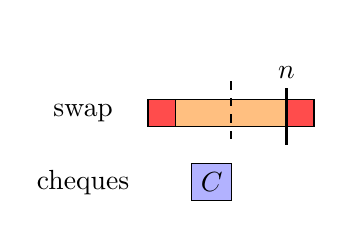
\begin{tikzpicture}
\node (middle)[draw, rectangle, fill=orange!50, minimum height=1em, minimum width=4em]{};
\node (leftred) [draw, rectangle, fill=red!70, minimum height=1em, minimum width=1em, node distance=2.5em, left of=middle]{};
\node (rightred)[draw, rectangle, fill=red!70, minimum height=1em, minimum width=1em, node distance=2.5em, right of=middle]{};
\node (zero) [above of=middle,node distance=2em, text height=1em] {};
\node (zerod) [below of=zero, node distance=3.5em] {};
\node (balance) [right of=zero,node distance=2em, text height=1.5em] {$n$};
\node (balanced) [below of=balance,node distance=3.5em] {};
\draw [dashed](zero)--(zerod);
\draw [very thick](balance)--(balanced);
\node (payment) [below of=zerod, node distance=1em]{};
\node (cheqeue) [draw, left of=payment, node distance=.7em, minimum height=1em, minimum width=1.4em, fill=blue!30, rectangle]{$C$};

\node (swap) [left of=leftred,minimum width=1em,align=right]{swap};
\node (cheques) [below of=swap,minimum width=1em, node distance= 2.5em, align=right]{cheques};
\end{tikzpicture}
&
\begin{tabular}{c}
  $\Longrightarrow$
\\ \\ \\ \\
\end{tabular}
&
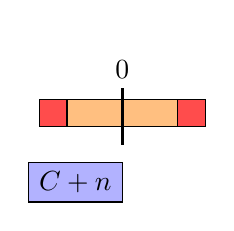
\begin{tikzpicture}
\node (middle)[draw, rectangle, fill=orange!50, minimum height=1em, minimum width=4em]{};
\node (leftred) [draw, rectangle, fill=red!70, minimum height=1em, minimum width=1em, node distance=2.5em, left of=middle]{};
\node (rightred)[draw, rectangle, fill=red!70, minimum height=1em, minimum width=1em, node distance=2.5em, right of=middle]{};
\node (zero) [above of=middle,node distance=2em, text height=1.5em] {$0$};
\node (zerod) [below of=zero, node distance=3.5em] {};
% \draw [dashed](zero)--(zerod);
\draw [very thick](zero)--(zerod);
\node (payment) [below of=zerod, node distance=1em]{};
\node (cheque) [draw, left of=payment, node distance=1.7em, minimum height=1em, minimum width=3.4em, fill=blue!30, rectangle]{$C+n$};
\end{tikzpicture}
\end{tabular}
\end{center}

\caption[Cheque swap]{Peer B's swap balance (with respect to A) reaches the payment threshold (left),
B sends a cheque to peer A. B keeps the cheque and restores the swap balance to zero.}
\label{fig:chequeswap}
\end{figure}
\end{center}

\subsection{Cheques as off-chain commitments to pay}\label{sec:cheques}

One of the major issues with direct "on-chain" payments in a blockchain network is that each transaction must be processed by each and every node participating in the network, resulting in high transaction costs. It is possible to create a payment without presenting this payment on-chain. Such payments are called second-layer payment strategies. One such strategy is to defer payments and process them in bulk. In exchange for reduced cost, the beneficiary must be willing to incur higher risk of settlement failure. We argue that this is perfectly acceptable for bandwidth incentivisation where peers engage in repeated dealings.


\subsubsection{The chequebook contract}

A very simple smart contract that allows the beneficiary to choose when payments are to be processed was introduced in \cite{ethersphere2016sw3}. This \gloss{chequebook contract} is a wallet that can process cheques issued by its owner. The cheques are analogous to those in the real-world: The issuer signs a \emph{cheque} specifying a \emph{beneficiary}, a \emph{date} and an \emph{amount}, gives it to the recipient as a token of promise to pay at a later date. The smart contract plays the role of the bank. When the recipient wishes to get paid, they "cash the cheque" by submitting it to the smart contract. The contract, after validating the signature, date and the amount specified on the cheque, transfers the amount to the beneficiary's account (see figure \ref{fig:swap-chequebook}). Analogously to the person taking the cheque to the bank to cash it, anyone can send the digital cheque in a transaction to the owner's chequebook account and thus trigger the transfer. 

The swap protocol specifies that when the \emph{payment threshold} is exceeded, a cheque is sent over the creditor peer. Such cheques can be cashed immediately by being sent to the issuer's chequebook contract. Alternatively, cheques can also be withheld. Withholding a cheque is effectively lending on credit, which enables the parties to save on transaction costs. 

The amount deposited in the chequebook (\gloss{global balance}) serves as collateral for the cheques. It is pooled over the beneficiaries of all outstanding cheques. In this simplest form, the chequebook has the same guarantee as real-world cheques: None. Since funds can be freely moved out of the chequebook wallet at any time, solvency at the time of cashing can never be guaranteed: If the chequebook's balance is less than the amount sanctioned by a cheque submitted to it, the cheque will bounce. This is the trade off between transaction costs and risk of settlement failure.

While, strictly speaking, there are no guarantees for solvency, nor is there an explicit punitive measure on insolvency, a bounced cheque will affect the issuer's reputation as the chequebook contract records it. On the premise that cheques are swapped in the context of repeating dealings, peers will refrain from issuing cheques beyond their balance. In other words, interest in keeping good reputation with their peers serves as an incentive for nodes to maintain solvency.


\begin{figure}[htbp]
\centering
% Agents
\def\IssuerLocal{A client}
\def\IssuerSwapContract{A swap}
\def\BeneficiarySwapContract{B swap}
\def\BeneficiaryLocal{B client}

% Message Flows
\def\Issue{issue cheque}% \def\Cheque{Cheque}
\def\Redeem{redeem cheque} %\def\Cheque{Cheque}
\def\Clear{clear ETH} %\def\ETH{ETH}
\def\NW{withdrawal event} %\def\Msg{Log Event}
\def\ND{deposit event} %\def\Msg{Log Event}

% Legend 
\def\LegendOnChain{On-chain}
\def\LegendOffChain{Off-chain}


\begin{tikzpicture}[every node/.style={font=\small,
  minimum height=.35cm,minimum width=.5cm},]

%
% Matrix
\node [matrix, very thin,column sep=1.0cm,row sep=0.2cm] (matrix) at (0,0) {
  & \node(0,0) (\IssuerLocal) {};   &                         & \node(0,0) (\IssuerSwapContract) {};   & & \node(0,0) (\BeneficiarySwapContract) {};   & & \node(0,0) (\BeneficiaryLocal) {}; \\
  & & & & & & & \\
  & & & & & & & \\
  & & & & & & & \\
  & \node(0,0) (\IssuerLocal 1) {}; & \node(0,0) (\Issue) {}; & \node(0,0) (\IssuerSwapContract 1) {}; & & \node(0,0) (\BeneficiarySwapContract 1) {}; & & \node(0,0) (\BeneficiaryLocal 1) {}; \\
  & & & & & & & \\
  & & & & & & & \\
  & \node(0,0) (\IssuerLocal 2) {}; &                         & \node(0,0) (\IssuerSwapContract 2) {}; & & \node(0,0) (\BeneficiarySwapContract 2) {}; & \node(0,0) (\Redeem) {};  &  \node(0,0) (\BeneficiaryLocal 2) {}; \\ 
  & & & & & & & \\
  & & & & & & & \\
  & \node(0,0) (\IssuerLocal 3) {}; &                         & \node(0,0) (\IssuerSwapContract 3) {}; & \node(0,0) (\Clear) {}; & \node(0,0) (\BeneficiarySwapContract 3) {}; &                    ; & \node(0,0) (\BeneficiaryLocal 3) {}; \\
  & & & & & & & \\
  & \node(0,0) (\IssuerLocal 4) {}; & \node(0,0) (\NW) {}   ; & \node(0,0) (\IssuerSwapContract 4) {}; &                         & \node(0,0) (\BeneficiarySwapContract 4) {}; & \node(0,0) (\ND) {}; & \node(0,0) (\BeneficiaryLocal 4) {}; \\
  & & & & & & & \\
  & \node(0,0) (\IssuerLocal 5) {}; &                         & \node(0,0) (\IssuerSwapContract 5) {};  & & \node(0,0) (\BeneficiarySwapContract 5) {};& & \node(0,0) (\BeneficiaryLocal 5) {}; \\
  & & & & & & & \\
  & \node(0,0) (\IssuerLocal 6) {}; &                         & \node(0,0) (\IssuerSwapContract 6) {};  & & \node(0,0) (\BeneficiarySwapContract 6) {};& & \node(0,0) (\BeneficiaryLocal 6) {}; \\
  & & & & & & & \\
  & \node(0,0) (\IssuerLocal 7) {}; & \node(0,0) (\LegendOnChain) {};  & & & & & \\
  & \node(0,0) (\IssuerLocal 8) {}; & \node(0,0) (\LegendOffChain) {}; & & & & & \\
};

% Agents labels
\fill 
	(\IssuerLocal) node[draw,fill=white] {\IssuerLocal}
	(\IssuerSwapContract) node[draw,fill=white] {\IssuerSwapContract}
	(\BeneficiarySwapContract) node[draw,fill=white] {\BeneficiarySwapContract}
	(\BeneficiaryLocal) node[draw,fill=white] {\BeneficiaryLocal};

\draw [dashed] 
  (\IssuerLocal) -- (\IssuerLocal 6)
  (\BeneficiaryLocal) -- (\BeneficiaryLocal 6)
  (\IssuerSwapContract) -- (\IssuerSwapContract 6)
  (\BeneficiarySwapContract) -- (\BeneficiarySwapContract 6);

% Horizontal flows (Monetary interactions)
%\draw [-latex] (\IssuerLocal 1) -- (\IssuerSwapContract 1.west) arc(180:0:0.37cm) -- (\BeneficiarySwapContract 1.west) arc(180:0:0.37cm) -- (\BeneficiaryLocal 1);
\draw [-{Latex[length=1.5mm,width=2.5mm]}] (\IssuerLocal 1) -- (\BeneficiaryLocal 1);
\draw [-{Latex[length=1.5mm,width=2.5mm]}] (\BeneficiaryLocal 2) -- (\IssuerSwapContract 2);
%\draw [-latex] (\BeneficiaryLocal 2) -- (\BeneficiarySwapContract 2.east) arc(0:180:0.37cm) -- (\IssuerSwapContract 2);
\draw [-{Latex[length=1.5mm,width=2.5mm]}] (\IssuerSwapContract 3) -- (\BeneficiarySwapContract 3);
\draw [-{Latex[length=1.5mm,width=2.5mm]}] (\IssuerSwapContract 3) -- (\IssuerLocal 4);
\draw [-{Latex[length=1.5mm,width=2.5mm]}] (\BeneficiarySwapContract 3) -- (\BeneficiaryLocal 5);

% Flows Labels 
\fill
  (\Issue) 
    node[above, font=\footnotesize ] {\Issue}
  (\Redeem) 
    node[above, font=\footnotesize] {\Redeem}
  (\Clear) 
    node[above, font=\footnotesize] {\Clear}
  (\NW) 
    node[above, font=\footnotesize, text width=1.4cm, text height=1.5cm, align=center,fill=white] {\NW}
  (\ND) 
    node[above, font=\footnotesize, text width=1.5cm,align=center,fill=white] {\ND};

% Interaction points 
\draw 
  (\IssuerLocal 1) node[minimum size=0.25cm, draw,circle,fill=red!20] {}
  (\BeneficiaryLocal 1) node[minimum size=0.25cm, draw,circle,fill=red!20] {}
  (\BeneficiaryLocal 2) node[minimum size=0.25cm, draw,circle,fill=red!20] {}
  (\IssuerSwapContract 2) node[minimum size=0.25cm, draw,circle,fill=green!20] {}
  (\IssuerSwapContract 3) node[minimum size=0.25cm, draw,circle,fill=green!20] {}
  (\IssuerLocal 4) node[minimum size=0.25cm, draw,circle,fill=red!20] {}
  (\BeneficiarySwapContract 3) node[minimum size=0.25cm, draw,circle,fill=green!20] {}
  (\BeneficiaryLocal 5) node[minimum size=0.25cm, draw,circle,fill=red!20] {}
  (\IssuerLocal 7) node[minimum height=.1cm, minimum size=0.1cm, draw,circle,fill=green!20] {}
  (\IssuerLocal 8) node[minimum height=.1cm, minimum size=0.1cm, draw,circle,fill=red!20] {};

% Vertical lifelines
\draw [-{Latex[length=1.5mm,width=2mm]}] (\IssuerSwapContract 2) -- (\IssuerSwapContract 3);
 Legend labels
\draw
	(\LegendOnChain) node[minimum height=.1cm] {\LegendOnChain}
	(\LegendOffChain) node[minimum height=.1cm] {\LegendOffChain};
\end{tikzpicture}

\caption[The basic interaction sequence for swap chequebooks]{The basic interaction sequence for swap chequebooks}
\label{fig:swap-chequebook}
\end{figure}


\subsubsection{Double cashing}

Since these digital cheques are files and can therefore be copied, care must be taken that the same cheque cannot be cashed twice. Such "double cashing" can be prevented by assigning each cheque given to a particular beneficiary a serial number which the contract will store when the cheque is cashed. The chequebook contract can then rely on the serial number to make sure cheques are cashed in sequential order, thus needing to store only a single serial number per beneficiary.

An alternative strategy to prevent double cashing, when repeated payments are made to the same beneficiary, is that the cheques contain the \emph{cumulative} total amount ever credited to the beneficiary. The total  amount that has been cashed out is stored in the contract for each beneficiary. When a new cheque is submitted, the contract ignores cheques with amount equal to or less than the stored total, but it will transfer the difference if it receives a cheque with a higher total.


This simple trick also makes it possible to cash cheques in bulk because only the current "last cheque" need ever be processed. This achieves the reduction of transaction costs alluded to above.

\subsubsection{Cashing without Ether}\label{sec:zero_eth}
Not all peers in Swarm are expected to have the Ether needed to pay for the transaction costs to cash out a cheque. The chequebook allows third parties to cash cheques. The sender of the transaction is incentivized with a reward for the service performed.

\subsection{Waivers}\label{sec:waiver}

If the imbalance in the swap channel is the result of high variance as opposed to unequal consumption, after a period of accumulating cheques the channel balance starts tilting the other way. Normally, it is now up to the other party to issue cheques to its peer resulting in uncashed cheques accumulating on both sides.
To allow for further savings in transaction costs, it could be desirable to be able to "play the cheques off against each other".

Such a process is possible, but it requires certain important changes within the chequebook contract. In particular, cashing cheques can no longer be immediate and must incur a security delay, a concept familiar from payment channels.

Let us imagine a system analogous to cheques being returned to the issuer. Assume peer A issued cheques to B and the balance was brought back to zero. Later the balance tilts in A's favour but the cheques from A to B have not been cashed. In the real world, user B could simply return the last cheque back to A or provably destroy it. In our case it is not so simple; we need some other mechanism by which B \emph{commits not to cash} that particular cheque. Such a commitment could take several forms; it could be implemented by B signing a message allowing A to issue a new `last cheque` which has a lower cumulative total amount than before, or perhaps B can issue some kind of `negative` cheque for A's chequebook that would have the effect as if a cheque with the same amount had been paid. 

What all the implementations have in common, is that the chequebook can no longer allow instantaneous cashing of cheques. Upon receiving a cheque cashing request, the contract must wait to allow the other party in question to submit potentially missing information about cancelled cheques or reduced totals. To accommodate (semi-)bidirectional payments using a single chequebook we make the following modifications:

\begin{enumerate}
    \item All cheques from user A to user B must contain a serial number.
    \item Each new cheque issued by A to B must increase the serial number.
    \item A's chequebook contract records the serial number of the last cheque that B cashed.
    \item During the cashing delay, valid cheques with higher serial number supersede any previously submitted cheques regardless of their face value.
    \item Any submitted cheque which decreases the payout of the previously submitted cheque is only valid if it is signed by the beneficiary.
\end{enumerate}


\begin{figure}[htbp]
\centering
% Waivers diagram 
% Author: Fabio Barone, based on Pascal Seppecher taken from http://www.texample.net/tikz/examples/sequence-diagram/

% Agents
\def\A{A}
\def\B{B}
\def\FaceVal{Amount due}
\def\Contract{Contract value}
\def\Totals{Cumulative Sum}

% Message Flows
\def\ChequeA{Cheque $c0$}
\def\ChequeB{Cheque $c1$}
\def\ChequeC{Cheque $c2$}
\def\RedeemC{Redeem Cheque $c1$}
\def\ChequeD{Cheque $c3$}
\def\WFailCumTotTooHigh{Waive attempt $w_4$}
\def\WaiverA{Waive $w_4$}
\def\RedeemFailWrongSN{Redeem $c3$}
\def\WaiverB{Waive $w_5$}
\def\ChequeE{Cheque $c6$}
\def\ChequeF{Cheque $c7$}
\def\RedeemF{Redeem $c7$}
\def\ChequeG{Cheque $c8$}
\def\RedeemG{Redeem $c8$}

% Legend 
%\def\LegendOnChain{On-chain}
%\def\LegendOffChain{Off-chain}

\begin{tikzpicture}[every node/.style={font=\small,
  minimum height=.35cm,minimum width=.5cm}]
 \useasboundingbox (-1cm,-7cm) rectangle (3.5cm,7cm);
   \scope[transform canvas={scale=.75}]


%
% Matrix
\node [matrix, very thin,column sep=2.0cm,row sep=0.4cm] (matrix) at (0,0) {
  &  & \node(0,0) (\A) {}; &                        & \node(0,0) (\B) {};        & \node(0,0) {Serial};               & \node(0,0) (\FaceVal) {};  & \node(0,0) (\Contract) {}; & \node(0,0) (\Totals) {}; \\
  &  & & & & & & &  \\
  &  & & & & & & &  \\
  &  & & & & & & & \\
  &  & \node(0,0) (\A 1) {}; & \node(0,0) (\ChequeA) {}; & \node(0,0) (\B 1) {};& \node(0,0) {0};                    & \node(0,0) {6};          & \node(0,0) {6};            & \node(0,0) {6}; \\
  &  & & & & & & & \\
  &  & \node(0,0) (\A 2) {}; & \node(0,0) (\ChequeB) {}; & \node(0,0) (\B 2) {};& \node(0,0) {1};                     & \node(0,0) {9};          & \node(0,0) {15};            & \node(0,0) {15}; \\ 
  &  & & & & & & & \\
  &  & \node(0,0) (\A 3) {}; & \node(0,0) (\ChequeC) {}; & \node(0,0) (\B 3) {};& \node(0,0) {2};                     & \node(0,0) {13};          & \node(0,0) {28};            & \node(0,0) {28}; \\
  &  & & & & & & & \\
  &  & \node(0,0) (\A 4) {}; & \node(0,0) (\RedeemC) {}; & \node(0,0) (\B 4) {};& \node(0,0) {1};                 & \node(0,0) {15};          & \node(0,0) {19};            & \node(0,0) {28}; \\
  &  & & & & & & & \\
  &  & \node(0,0) (\A 5) {}; & \node(0,0) (\ChequeD) {}; & \node(0,0) (\B 5) {};& \node(0,0) {3};                     & \node(0,0) {14};          & \node(0,0) {33};            & \node(0,0) {42}; \\
  & & & & & & & & \\
  & \node(0,0) {Fails as exceeds Contract value} ;  & \node(0,0) (\A 6) {}; & \node(0,0) (\WFailCumTotTooHigh) {}; & \node(0,0) (\B 6) {}; & \node(0,0) {4};    & \node(0,0) {100};          & \node(0,0) {33};            & \node(0,0) {42}; \\
  &  & & & & & & & \\
  &  & \node(0,0) (\A 7) {}; & \node(0,0) (\WaiverA) {}; & \node(0,0) (\B 7) {};& \node(0,0) {4};                     & \node(0,0) {7};          & \node(0,0) {26};            & \node(0,0) {42}; \\
  &  & & & & & & & \\
  & \node(0,0) {Fails due to wrong s/n}; & \node(0,0) (\A 8) {}; & \node(0,0) (\RedeemFailWrongSN) {}; & \node(0,0) (\B 8) {};& \node(0,0) {3};      & \node(0,0) {42};          & \node(0,0) {26};            & \node(0,0) {42}; \\
  &  & & & & & & & \\
  &  & \node(0,0) (\A 9) {}; & \node(0,0) (\WaiverB) {}; & \node(0,0) (\B 9) {};& \node(0,0) {5};                     & \node(0,0) {26};          & \node(0,0) {0};            & \node(0,0) {42}; \\
  &  & & & & & & & \\
  &  & \node(0,0) (\A 10) {}; & \node(0,0) (\ChequeE) {}; & \node(0,0) (\B 10) {};& \node(0,0) {6};                     & \node(0,0) {11};          & \node(0,0) {11};            & \node(0,0) {53}; \\
  &  & & & & & & & \\
  &  & \node(0,0) (\A 11) {}; & \node(0,0) (\ChequeF) {}; & \node(0,0) (\B 11) {};& \node(0,0) {7};                     & \node(0,0) {15};          & \node(0,0) {26};            & \node(0,0) {68}; \\
  &  & & & & & & & \\
  &  & \node(0,0) (\A 12) {}; & \node(0,0) (\RedeemF) {}; & \node(0,0) (\B 12) {};& \node(0,0) {7};               & \node(0,0) {68};          & \node(0,0) {0};            & \node(0,0) {68}; \\
  &  & & & & & & & \\
  & \node(0,0) {Exchange in other direction ok};   & \node(0,0) (\A 13) {}; & \node(0,0) (\ChequeG) {}; & \node(0,0) (\B 13) {};& \node(0,0) {0};                     & \node(0,0) {};          & \node(0,0) {};            & \node(0,0) {}; \\
  &  & & & & & & & \\
  &  & \node(0,0) (\A 14) {}; & \node(0,0) (\RedeemG) {}; & \node(0,0) (\B 14) {}; & \node(0,0) {1};              & \node(0,0) {};          & \node(0,0) {};            & \node(0,0) {}; \\
  &  & & & & & & & \\
  &  & \node(0,0) (\A 15) {}; &                          ; & \node(0,0) (\B 15) {};&                               &                           &                             &                  \\
};

% Agents labels
\fill 
	(\A) node[draw,fill=white] {\A}
	(\B) node[draw,fill=white] {\B}
	(\FaceVal) node[] {\FaceVal}
	(\Contract) node[] {\Contract}
	(\Totals) node[] {\Totals};

\draw [dashed] 
  (\A) -- (\A 15)
  (\B) -- (\B 15);

% Horizontal flows 
\draw [-{Latex[length=1.5mm,width=2.5mm]}] (\A 1) -- (\B 1);
\draw [-{Latex[length=1.5mm,width=2.5mm]}] (\A 2) -- (\B 2);
\draw [-{Latex[length=1.5mm,width=2.5mm]}] (\A 3) -- (\B 3);
\draw [-{Latex[length=1.5mm,width=2.5mm]}] (\B 4) -- (\A 4);
\draw [-{Latex[length=1.5mm,width=2.5mm]}] (\A 5) -- (\B 5);
\draw [-{Latex[length=1.5mm,width=2.5mm]},color=red] (\B 6) -- (\A 6);
\draw [-{Latex[length=1.5mm,width=2.5mm]}] (\B 7) -- (\A 7);
\draw [-{Latex[length=1.5mm,width=2.5mm]},color=red] (\B 8) -- (\A 8);
\draw [-{Latex[length=1.5mm,width=2.5mm]}] (\B 9) -- (\A 9);
\draw [-{Latex[length=1.5mm,width=2.5mm]}] (\A 10) -- (\B 10);
\draw [-{Latex[length=1.5mm,width=2.5mm]}] (\A 11) -- (\B 11);
\draw [-{Latex[length=1.5mm,width=2.5mm]}] (\B 12) -- (\A 12);
\draw [-{Latex[length=1.5mm,width=2.5mm]}] (\A 13) -- (\B 13);
\draw [-{Latex[length=1.5mm,width=2.5mm]}] (\B 14) -- (\A 14);

% Flows Labels 
\fill
  (\ChequeA) 
    node[above] {\ChequeA}
  (\ChequeB) 
    node[above] {\ChequeB}
  (\ChequeC) 
    node[above] {\ChequeC}
  (\RedeemC) 
    node[above] {\RedeemC}
  (\ChequeD) 
    node[above] {\ChequeD}
  (\WFailCumTotTooHigh) 
    node[above] {\WFailCumTotTooHigh}
  (\WaiverA) 
    node[above] {\WaiverA}
  (\RedeemFailWrongSN) 
    node[above] {\RedeemFailWrongSN}
  (\WaiverB) 
    node[above] {\WaiverB}
  (\ChequeE) 
    node[above] {\ChequeE}
  (\ChequeF) 
    node[above] {\ChequeF}
  (\RedeemF) 
    node[above] {\RedeemF}
  (\ChequeG) 
    node[above] {\ChequeG}
  (\RedeemG) 
    node[above] {\RedeemG};

% Interaction points 
\draw 
  (\A 1) node[minimum size=0.25cm, draw,circle,fill=red!20] {}
  (\B 1) node[minimum size=0.25cm, draw,circle,fill=red!20] {}
  (\A 2) node[minimum size=0.25cm, draw,circle,fill=red!20] {}
  (\B 2) node[minimum size=0.25cm, draw,circle,fill=red!20] {}
  (\A 3) node[minimum size=0.25cm, draw,circle,fill=red!20] {}
  (\B 3) node[minimum size=0.25cm, draw,circle,fill=red!20] {}
  (\A 4) node[minimum size=0.25cm, draw,circle,fill=red!20] {}
  (\B 4) node[minimum size=0.25cm, draw,circle,fill=red!20] {}
  (\A 5) node[minimum size=0.25cm, draw,circle,fill=red!20] {}
  (\B 5) node[minimum size=0.25cm, draw,circle,fill=red!20] {}
  (\A 6) node[minimum size=0.25cm, draw,circle,fill=red!20] {}
  (\B 6) node[minimum size=0.25cm, draw,circle,fill=red!20] {}
  (\A 7) node[minimum size=0.25cm, draw,circle,fill=red!20] {}
  (\B 7) node[minimum size=0.25cm, draw,circle,fill=red!20] {}
  (\A 8) node[minimum size=0.25cm, draw,circle,fill=red!20] {}
  (\B 8) node[minimum size=0.25cm, draw,circle,fill=red!20] {}
  (\A 9) node[minimum size=0.25cm, draw,circle,fill=red!20] {}
  (\B 9) node[minimum size=0.25cm, draw,circle,fill=red!20] {}
  (\A 10) node[minimum size=0.25cm, draw,circle,fill=red!20] {}
  (\B 10) node[minimum size=0.25cm, draw,circle,fill=red!20] {}
  (\A 11) node[minimum size=0.25cm, draw,circle,fill=red!20] {}
  (\B 11) node[minimum size=0.25cm, draw,circle,fill=red!20] {}
  (\A 12) node[minimum size=0.25cm, draw,circle,fill=red!20] {}
  (\B 12) node[minimum size=0.25cm, draw,circle,fill=red!20] {}
  (\A 13) node[minimum size=0.25cm, draw,circle,fill=red!20] {}
  (\B 13) node[minimum size=0.25cm, draw,circle,fill=red!20] {}
  (\A 14) node[minimum size=0.25cm, draw,circle,fill=red!20] {}
  (\B 14) node[minimum size=0.25cm, draw,circle,fill=red!20] {};

% Vertical lifelines
\endscope
\end{tikzpicture}

\caption[Example sequence of mixed cheques and waivers exchange]{Example sequence of mixed cheques and waivers exchange}
\label{fig:waivers-diagram}
\end{figure}

With these rules in place it is easy to see how cheque cancellation would work. Suppose user A has issued cheques $c_0 \ldots c_n$ with cumulative totals $t_0 \ldots t_n$ to user B. Suppose that the last cheque B cashed was $c_i$. The chequebook contract has recorded that B has received a payout of $t_i$ and that the last cheque cashed had serial number $i$.

Let us further suppose that the balance starts tilting in A's favour by some amount $x$. If B had already cashed cheque $c_n$, then B would now have to issue a cheque of her own using B's chequebook as the source and naming A as the beneficiary. However, since cheques $c_{i+1} \ldots c_n$  are uncashed, B can instead send to A a cheque with A's chequebook as the source, B as the beneficiary, with serial number $n+1$ and cumulative total $t_{n+1} = t_n - x$. Due to the rules enumerated above, A will accept this as equivalent to a payment of amount $x$ by B.  In this scenario, instead of sending a cheque to A, B waive part of their earlier entitlement. This justifies swap as \emph{send waiver as payment}.

This process can be repeated multiple times until the cumulative total is brought back to $t_i$. At this point all outstanding debt has effectively been cancelled and any further payments must be made in the form of a proper cheque from B's chequebook to A (see figure \ref{fig:waivers-diagram}).


\subsection{Zero cash entry}\label{sec:zero-cash-entry}


Swap accounting can also work in one direction only. If a party enters the system with zero liquid capital (\gloss{newcomer}), but connects to peers with funds (\gloss{insider}), the newcomer begins to provide the service (and not use it) in order to earn a positive swap balance. 

If the insider has a chequebook they can pay the newcomer with a cheque. This has a caveat: The newcomer will be  able to earn cheques for services provided, but will not have the means to cash them. Cashing cheques requires sending a transaction to the blockchain, and therefore requires gas.  Unless the  node can convince one of its peers to send the transaction for them. We allow nodes to sign off on a structure that they want sent, and extend the swap contract with a preprocessing step, which triggers payment to the transaction sender covering the transaction’s gas cost plus a service fee. The newcomer's cheque can be cashed by any insider (see figure \ref{fig:zero-cash-entry}). This feature justifies swap as \emph{start without a penny, send with a peer}.

\begin{figure}[htbp]
\centering
\input{fig/zero-cash-entry.tex}
\caption[Zero cash entry]{Bootstrapping or how to launch as a swap capable node consuming and providing a
service and earn money.}
\label{fig:zero-cash-entry}
\end{figure}

The possibility to earn small amounts of money without starting capital is important, as it provides a way to get access to Swarm without the need to purchase the token. This benefit extends to the Ethereum ecosystem in general: with Swarm, anybody can earn small amounts of money to start paying the gas for their dapps, without the need to go through the pain full process of acquiring tokens. 

\subsection{Sanctions and blacklisting}\label{sec:sanctions}
\red{}
\subsubsection{Protocol breach}

\subsubsection{Excessive frivolity}

\subsubsection{Quality of service}

measures - need no distinction between malicious attacks or suboptimal (poor quality, overpriced) service provided in good faith.

\subsubsection{Blacklisting}

\section{Storage incentives}\label{sec:storage-incentives}

\wip{the lottery is not completely finalised}

In \ref{sec:postage-stamps}, we introduce postage stamps, primarily as a measure against spam protection.  
We then turn to postage lottery explaining how postage stamps used for spam protection can be modified to give positive incentives to nodes to store files and indicate their importance (\ref{sec:postage-lottery}). In \ref{sec:capacity-pressure} we describe how the pricing mechanism can be used to signal capacity pressure of the network and how the incentives work to rectify that. Finally, \ref{sec:chunk-insurance} shows how positive rewards of the postage lottery can be complemented by introducing staked insurers who stand to lose their deposit if they lose chunks they insured. We argue that such punitive measures are crucial in mitigating the tragedy of commons problem in systems with positive storage incentives only. 

\subsection{Spam protection with postage stamps}\label{sec:postage-stamps}
\green{}

Syncing involves transferring chunks from the uploader to storers, i.e., to the neighbourhood where the chunk falls within the nodes' area of responsibility. Storer nodes aspire to serve content as a response to retrieve requests. All else being equal, given Kademlia routing, the closer a node is to the chunk address, the more likely it is that a request for that chunk will end up with them. This creates a weak incentive for storer nodes to sync content. However, it presupposes that the chunk has the promise of some profit. This assumption is not warranted if an adversary can spam the network with chunks (maybe randomly generated) that are never requested. From the network's point of view, this means that useless chunks replace useful ones. Attaching a cost to uploading a chunk to Swarm can mitigate such an attack. 


\subsubsection{Postage stamps}

Taking inspiration from international mail delivery, the entire delivery path (as well as storage) can be pre-paid and the proof of payment called a \gloss{postage stamp} needs to be attached to the payload by the sender.

This cost need not necessarily be borne by the uploaders but they are the ones that need to make sure the postage stamp is attached to each chunk,  otherwise the upload will not succeed. Conversely, the inpayment need not necessarily be paid out as revenue to anyone in particular, i.e., it can be burnt or otherwise redistributed. The actual cost of uploading a chunk can serve as a signal of importance (somewhat analogously to priority mail) that storer nodes can use to rank chunks when selecting which one to garbage collect (see \ref{spec:strategy:garbage-collection}) in the event of capacity shortage.

A postage stamp is modelled by a proof of payment associated with a chunk using a \gloss{witness}. The witness is implemented as the digital signature issued by the entity that the payer designates.


\subsubsection{Proof of payment}

The proof of payment can lend itself to a number of different implementations. The most obvious choice is to make payments to a central postage stamp issuer smart contract on the blockchain.%
%
\footnote{Using a cheque seems one option, however, cheques are  signed against cumulative debt and therefore assume the single beneficiary is able to reconstruct the added value over the previously sent cheque. In other words, cheques are not appropriate to communicate value to non-peers.}
%
Because of the high transaction cost, requiring an on-chain payment for each chunk is prohibitively expensive. Instead, we need a solution that allows the uploader to purchase the postage stamps in a \emph{batch} and reuse it over several chunks. 


The batches are created by a central postage smart contract when a transaction is sent to its create endpoint with an amount of honey tokens and the following transaction data;

\begin{itemize}
\item \emph{owner address} - The owner that is entitled to use the batches created to stamp chunks.
\item \emph{number of batches} - Number of batches to be created by this payment.
\item \emph{batch depth} - Log number of chunks that can be stamped with each batch created.
\end{itemize}

This postage payment results in the following information being recorded:

\begin{itemize}
\item \emph{payment reference ID} - A random ID generated as reference for this payment.
\item \emph{per-chunk balance} - Total amount equally allocated for chunks covered by the batches created from this payment.
\item \emph{owner address} - The owner that is entitled to use the batches created to stamp chunks.
\item \emph{number of batches} - Number of batches created by this payment.
\item \emph{batch depth} - Log number of chunks that can be stamped with each batch created.
\end{itemize}

The payment transaction will create multiple batches the number of which is specified in the transaction. The batch depth is fixed at any moment in time by the contract itself as explained below. Since it can change and it can influence how many stamps owner can issue, it is also specified in the transaction. If there is a mismatch the transaction is rejected.
The owner is an address specified in the transaction data and recorded as the party authorised to use the batches created to stamp chunks; if not specified, it is the transaction sender by default. A random identifier is generated to reference the payment. The number of batches created and the batch depth used gets recorder for the payment ID. These two multiplied is the number of chunks covered by this payment. The amount of honey sent in with the transaction gets allocated equally to all chunks covered by the payment, i.e., the amount divided by the number of chunks covered is assigned to the payment ID to represent the per-chunk balance of the batches. Anyone can top up this balance at a later date. 

The postage stamp attached to a chunk is a data structure with the following fields (see more detail in \ref{spec:format:postage-stamps}):

\begin{itemize}
    \item \emph{chunk address} - The address the stamp is attached to. 
    \item \emph{batch identifier} - Composed of a payment identifier and a batch index validity of which can be checked with the postage smart contract.
    \item \emph{witness} - Owner's signature linking the batch identifier and the address.
\end{itemize}

The \emph{value} of a postage stamp is the per-chunk balance associated with the batch.
Similarly to stamps used for postal mail, a single chunk can have multiple postage stamps attached to it. In this case the value conferred to the chunk by multiple valid postage stamps simply add up. 

\subsubsection{Validity of postage stamp}

A postage stamp is valid if:

\begin{itemize}
\item \emph{authentic} - The batch identifier is valid, i.e., the payment ID exists and registered, the batch index is less than the number of batches associated with the payment ID.
\item \emph{authorised} - The witness is signed by the address specified as the owner of the batch.
\item \emph{funded} - The referenced batch has not exhausted its balance. 
\end{itemize}

All this can be checked by the smart contract. 
Validating that not more chunks are stamped with a batch than is allowed is important. Without further measures, there could be a possibility for an overspend attack in which the uploader reuses the stamp over more chunks than the  batch size would warrant and thereby  trick the unsuspecting storers into underpaid extra work. 

Protection against such \emph{overissuance} is not trivial: In the absence of global visibility of all chunks signed with a particular batch, nodes cannot directly verify the size, as they have no access to postage stamps attached to chunks not relayed through them. There needs to be a way for nodes to prevent overissuance collectively while each can act based only on locally available information.

\subsubsection{Limiting batch size based on sample estimate}
One solution is based on the realisation that estimation of absolute value densities is strictly speaking unnecessary. Nodes only want to prioritize chunks in case of resource shortage and for ranking chunks, comparison of the relative value densities of postage stamps that they have is sufficient.  This relative density is calculated by taking the number of chunks sharing the same postage stamp in the node's local storage. The reason this is a good enough strategy is apparent if we investigate how the uploader can manipulate the relative rank of their postage. If these cardinalities are uniform across nodes, then the estimation is both correct and consensual. Given chunk addresses are uniformly distributed, if chunks are randomly assigned to available postage stamps, on average an equal number of chunks will land in every neighbourhood. All the malicious uploader can do is artificially increase the density in certain neighbourhoods. However, such  manipulation can only lead to a situation where the target neighbourhood underestimates the relative value of the postage stamps. This will result in a lower rank for the chunks using the same stamp leading to earlier garbage collection and can ultimately only  hurt the uploader.

\subsubsection{Limiting batch size by constraining prefix collisions}

Another solution is to impose an explicit \gloss{uniformity requirement} on the batches: a constraint that chunks signed with the same batch identifier have no \gloss{prefix collision} longer than the depth. A postage stamp with a batch size of $2^d$ can be thought of as a balanced binary tree of depth $d$, where the leaves correspond to maximum length \glossplural{collision slot} of the batch. If the depth of a batch is greater than the depth of the network (log of the number of nodes in the network), then all chunks matching the same collision slot are guaranteed to land in the same neighbourhoods, and, as a result, "violations" of the uniformity requirement will be locally detected by nodes (see figure \ref{fig:prefix-collision}). If storers respond to this violation by randomly keeping only one of the chunks for each collision slot, uploaders will not only lose one chunk but also some predictability on top.

\begin{figure}[htbp]
  \centering
  \caption[Limiting the size of a postage stamp]{Limiting the size of a postage stamp by constraining the length of prefix collisions.}
  \label{fig:prefix-collision}
\end{figure}


As chunk addresses are never perfectly distributed over the collision slot of a batch, an uploader needs more than one batch of depth $d$ to sign $2^d$ chunks. In general, the best utilisation of the stamp is filling all the different collision slots (see \ref{sec:upload}). Put differently, continued non-uniformity will lead to underutilised stamps and therefore higher unit price for uploading and storing a chunk. This solution has the desired side effect that it imposes an upfront cost to non-uniform uploads: the more focused our upload is on a neighbourhood, the more slots of the postage stamps remain unused. As a consequence, directing uploads to a neighbourhood is expensive.%
%
\footnote{The cost of targeted attacks DDOSing neighbourhoods only is exponential in the depth.}
%
This will be significant for the discussion of decentralised file insurance (see \ref{sec:insurance}). 

An advantage of limiting batch size based on prefix collisions, over limiting batch size based on sample estimates is that with prefix collisions the absolute value of a postage stamp can be estimated, which comes in handy when designing the postage lottery (see: \ref{sec:postage-lottery}). 


In order for the collisions to be detectable, batch size needs to be higher than the estimated neighbourhood depth over the lifetime of the batch. It is not the interest of users to have batches much deeper than that, since the longer the collision prefixes, the more difficult it is achieve uniformity and to fill the entire batch. We will just assume for now that the depth of a batch is a fixed number set centrally on the contract and follows the depth of Swarm. The effect of network growth on the already used stamps is discussed below.


\subsubsection{Mining chunks using encryption}

Another solution to completely fill up postage batches relies on the insight hinted at in \ref{sec:chunk-encryption}: Choosing the encryption key allows us to \emph{mine} a chunk to a postage batch.

The process of finding an encryption key to generate a content hash close to an address is similar to mining blocks on the blockchain. Chunk encryption requires a 32-byte key, which plays the role of the nonce: It provides enough entropy to guarantee that one is found such that the resulting encrypted chunk will hash to an address with a particular prefix or collision slot of an open postage batch. The difficulty of mining is determined by the batch depth. 

Consider the thrifty uploader that only has as many postage collision slots as chunks. Given a postage stamp batch with depth $d$, they encrypt the chunk with a key chosen so that the resulting encrypted chunk's address fills a free collision slot of an open postage batch. As shown in the  appendix  (\ref{sec:complexity-filling}), this strategy of filling a batch requires on average $0.69d+1$ trials per chunk, i.e., 8, 15, 22 for thousand, million  and billion nodes respectively, which is reasonable.


\subsection{Postage lottery: positive incentives for storage}\label{sec:postage-lottery}

\yellow{}

As discussed in \ref{sec:accounting}, the primary incentive mechanism in Swarm is compensation for retrieval where nodes are rewarded for successfully serving a chunk. This reward mechanism has the added benefit of encouraging opportunistic caching. Profit-maximising storage nodes serve chunks they are often queried for and as a result, ensure that popular content becomes widely distributed and their retrieval latency is decreased.

The flipside of using this incentive only is that chunks that are rarely retrieved may end up lost. If a chunk is not being accessed for a long time, then as a result of limited storage capacity it will eventually end up garbage collected to make room for new arrivals. In order for the Swarm to guarantee long-term availability, the incentive system needs to make sure that additional revenue is generated for chunks that would otherwise be deleted. In other words, unpopular chunks that do not generate sufficient profit from retrievals should compensate the nodes that store them for their opportunities forgone. The \gloss{postage lottery} presented in this section provides such a compensation through redistributing the revenue coming from postage stamps among the registered storers in a fair way.



Implicit in our discussion of the bandwidth incentives for push-syncing, we assumed that  each chunk close to the storer constitutes an entitlement. Note, however, this does not mean that each chunk is a promise to be paid. Payouts can just as well be probabilistic as long as the expected revenue per chunk is the same and nodes have a clear way of estimating it. Using a lottery allows us to calibrate earnings that in the long run have the same payout as if there was an actual payment for each chunk, yet save on transaction costs.


\subsubsection{Automatic raffle rounds}

The postage lottery constitues of automatic raffle rounds and is managed by a smart contract on the EVM blockchain. The process is defined by the following protocol (see formally in \ref{spec:format:postage-stamps}). 

Every $N$-th block (on the Ethereum blockchain) represents a single global lottery draw, where the randomness comes from the previous block hash. This blockhash hashed together with the constants $c=0, 1, ..., n$ gives the \emph{node references} $n_c$, each defining an independent raffle.  From the network perspective, raffle rounds serve as spot checks on registered storer nodes, whereas for the latter they are the ways to secure their compensation for sharing disk space. 
Nodes whose address is in the close proximity to the node reference $n_i$ can apply to win the respective raffle round. The subsequent $N$ blocks are composed of three phases: 1) application 2) claim, and 3) challenge. The timeline of events is depicted in figure \ref{fig:raffle-timeline}.

\begin{figure}[htbp]
  \centering
  \caption[Timeline of events in a raffle round]{Timeline of events in a raffle round}
  \label{fig:raffle-timeline}
\end{figure}


\subsubsection{Applying for the prize}

To apply for the prize, the node needs to send a transaction to the lottery contract including a price offer for chunk per block. By submitting such a price, a node implicitly declares that it has in its possession all chunks of all batches with value higher than the price within their radius of responsibility. This radius is calculated based on the storers registered on the contract: the radius is the depth of the smallest neighbourhood such that it includes 1) the node reference, 2) the candidate node and 3) at least $r$ registered nodes, where $r$ is the Swarm  redundancy parameter (see figure \ref{fig:raffle-radius}). Nodes will have $N/3$ blocks after the raffle to submit a price.

\begin{figure}[htbp]
  \centering
  \caption[Radius of responsibility for postage lottery claims]{Radius of responsibility for postage lottery claims}
  \label{fig:raffle-radius}
\end{figure}

After this application deadline, the raffle enters the claim state. By hashing the blockhash at $N/3$ with constants $b=0, ..., m-1$, we generate $m$ \gloss{postage batch references}. Batch references are mapped to sample batches in the following way: Take the batch identifier that is closest to the reference $p_b$. This procedure selects a set of $m$ sample batches. To claim the raffle prize, a node needs to have all the chunks that they issued receipts for among the chunks stamped with each sample batch. 

\subsubsection{Claiming to be a winner}

As discussed previously, stamps attached to a  chunks endows the chunk with their value as defined by the batch balance per batch size. Pursuing a \gloss{value-consistent garbage collection strategy} (see \ref{spec:strategy:garbage-collection}) means the minimum postage stamp value accepted coincides with the maximum value ever deleted by the node. Nodes that follow this strategy know that they never deleted a chunk whose postage value was above their minimum required postage value. So they can be confident that they are able to include all relevant chunks of any postage batch above that value.

In order to prove possession, nodes must submit a batch proof of custody for each batch selected by the batch references. The \gloss{batch proof of custody} for a batch is a list of BMT proofs (see \ref{spec:format:bmt}) for all the chunks belonging to the batch that are in the applicant's area of responsibility and had been signed by the applicant. The chunks proofs are presented in a canonical order (see figure \ref{fig:batch-proof-of-custody}). Applicants have $N/3$ blocks to submit a claim, after which the raffle enters the challenge phase. Applicants that applied but fail to submit a claim are treated as if they submitted an invalid claim and will lose their registration.


\begin{figure}[htbp]
  \centering
  \caption{Batch proof of custody}
  \label{fig:batch-proof-of-custody}
\end{figure}

\subsubsection{Challenging the applicants}

If the set of chunks presented to the blockchain is incomplete, the applicants can be challenged on the blockchain by any third party submitting a statement of custody receipt signed by the applicant that is missing from the claim. The challenge is validated right away by the smart contract and if it is valid, the challenged applicant lose their registration immediately. Challengers have till the end of the raffle round (but at least $N/3$ blocks) to challenge applicants.

\subsubsection{Choosing the winner}

After the challenge phase ended ($N$ blocks after the beginning of the raffle round), among the applicants that survived the challenge, for each raffle, the ones that offered the lowest price win the round. 

The raffle prize paid out needs to take into account the number of winners, blocks and chunks.
The period paid is equally distributed among winners. For ease of reasoning, we can calibrate blocks = winners. The winner is entitled to collect the price for each chunk covered by the all postage batches. The sum of all winners' prices is subtracted from the remaining balance of each batch. The postage batches whose balance is dried after the payout are removed from the contract.

While winning nodes could benefit from a higher price for a bigger win, they are competing with each other to win the raffle so they are incentivised to secure their win by offering the actual cutoff value they used for garbage collection. As a result of competitive payouts, it is expected that the unit prices converge on the marginal cost  of storing one more chunk.

\subsubsection{Changing batch depth}


So far we just assumed that the batch depth was given by the contract. The requirement of batch depth is that it is deeper than the neighbourhood depth so that prefix collisions are caught by storer nodes, yet not too much deeper as that would make batches difficult to fill completely (see \ref{sec:complexity-filling}). If the collision slots of the batch have been completely filled, then the number of chunks per batch for a winner to show is expected to be on average $2^{d-b}$ where $b$ is the current batch depth and $d$ is the node's radius of responsibility (neighbourhood depth). Based on the actual number of chunks per batch ($C$) presented to the contract  by winners, we can have an estimate of the current neighbourhood depth in Swarm as $d'\defeq\mathit{log}_2(C)+b$. This gives the chance to the lottery smart contract to reset $b$ after each raffle so that it follows the neighbourhood depth, then no matter how Swarm is growing, the batch depth will have the required properties. 

Let us now investigate what happens to the value of an already existing batch if the official batch depth changes. If the batch depth increases, then a batch bought earlier when the depth was smaller, will behave as if it was a new batch not completely filled. This makes the reasoning about them relatively easy: with batch depth increased, the value of the postage decreases and the owner can act accordingly.

Practically old completely filled postage batches should either be retained or the content they cover should be reinsured (see figure  \ref{fig:filling-a-postage-batch}). In the former case, we want to retain the batch in case the batch depth grows and one can add chunks to it legitimately. In order to add new chunks to a batch without collisions, one needs to remember the chunks associated with the batch.%
%
\footnote{It is sufficient to just remember which collision slots were filled upto a depth possibly reached by a growing network. In practice, collision slots are recorded using a bit vector of length  $2^b$}
%
If the batch was filled completely at the time of upload and the batch is not retained, when batch depth increases, owner can just cash out from the batch, let its balance be drained and reupload with a new postage stamp.



\begin{figure}[htbp]
  \centering
  \input{fig/filling-a-postage-batch}
  \caption[Filling a postage batch]{Filling a postage batch.}
  \label{fig:filling-a-postage-batch}
\end{figure}


Note that owners can choose to pay for a postage an amount that even if  the Swarm grows on thousand fold, the balance runs dry only after a desired period. This is important in the context of \gloss{upload and disappear}.






\subsubsection{Statement of custody receipts}

Statement of custody receipts are crucial in the lottery, as they enable nodes to challenge. The challenge constitutes of submitting a receipt signed by the applicant. It is either a chunk closest to the applicant or to one of its neighbours. If the challenge is valid, the applicant loses their registered status. 

In order for syncing neighbours to be able to challenge, nodes need to attach a statement of custody receipt to all the chunks that they are closest to or their peer is closest to. The peers can be sanctioned with disconnection and blacklisting in case of non-compliance. 

As part of syncing, an aspiring storer node must sign statements of custody receipts for all the chunks that it is closest to. If the upstream peer did not require these, then they could not defend their territory as it were, i.e., they would have no grounds to challenge the new node when they apply for winning a raffle round after registering. Note that they do not need to keep all of them, since one is enough to challenge. The upstream node is not incentivised to withhold chunks that belong to the new node as they cannot earn from them any lottery winnings after the new node registers anyway. 

\subsubsection{Incentives implicit in the lottery}

This procedure incentivises nodes to adhere to the following behaviors:

\begin{itemize}
\item \emph{stay online} - Otherwise the raffle is missed.
\item \emph{have redundantly synced area of responsibility} - Remain fully synced with their neighbourhood. Otherwise the claim may be incomplete.
\item \emph{have a fully indexed local store} - To be able to list all chunks of a batch, nodes need to preserve postage stamps and keep an associated set of chunk addresses. In order to challenge frivolous registrants, nodes must keep receipts by neighbours.
\item \emph{perform value consistent garbage collection} - In order to tell if the node locally stores all previously receipted chunks of a batch they must perform garbage collection value-consistently,\footnote{or store indexes of deleted chunks which is inefficient}
i.e., the minimum value accepted coincides with the maximum value ever deleted.
\item \emph{store the data} - In order to provide BMT proofs the node needs to possess the data in the chunk content.\footnote{In the special case of addressed envelopes with prepaid postage, no payout can be collected before the envelope is filled and sent (see \ref{sec:addressed-envelopes}).}
\end{itemize}



\subsection{Price signalling capacity pressure}\label{sec:capacity-pressure}

\yellow{}

\subsubsection{Storage capacity}
Kademlia topology and the redundancy parameter determines the node's neighbourhood depth (see \ref{sec:redundancy-by-local-replication}). The neighbourhood depth delineates the area of responsibility. As a result of postage lottery, the nodes are incentivised to have a uniform neighbourhood size. The number of chunks uploaded to that area is simply proportional to the number of all chunks uploaded to Swarm $C$ and inversely proportional to the number of nodes in Swarm $N$. The number of chunks stored on a node is on average $CR/N$, where $R$ is the neighbourhood replication factor, measuring the degree of redundancy. expresses the density of chunks in any neighbourhood. Given a particular connectivity and fix storage for a neighbourhood, $C/N$ captures the \emph{storage capacity pressure}. 

If we assume that chunks are meant to be preserved only for a limited period of time, then within some variance the pressure stays constant. In other words, we can find a network size%
%
\footnote{in the sense of storage capacity; or in the sense of number of nodes assuming a minimum storage capacity per node.}
%
such that all content that users want preserved is preserved. 

If the rate of new uploads to Swarm is higher than the rate of expiry (postage stamp balances going below the current price), then a fixed network will experience increasing pressure. As a consequence, without added capacity, after a while, content that is meant to be preserved will be garbage collected. 

Such capacity shortage is solved if added storage is invited by incentivising new storer nodes to join the network or resist demand by raising prices. Conversely, if rate of expiry is faster than new uploads, pressure decreases and there may well be surplus capacity. The resulting situation with underutilised resources is remedied if added content is invited by incentivising users to upload their content or by some nodes dropping out disincentivised by lower prices. Thinking in terms of supply and demand, we can reach a self-regulating market simply if storage capacity pressure is signalled in the price of storage, i.e., minimum value for postage stamp per chunk. 

\subsubsection{Garbage collection strategy and postage value}

This is exactly what happens if the garbage collection queue is ordered by postage value (see \ref{spec:strategy:garbage-collection}).

\begin{figure}[htbp]
  \centering
  \caption{Garbage collection: chunks are ordered by profitability which comes from the postage value and a predicted retrieval revenue.}
  \label{fig:garbage-collection}
\end{figure}


Note that when a raffle round pays out, the same amounts get subtracted from all stamp balances. Therefore, the ordering by value does not change no matter how many raffle rounds happened. In order to insert a newly created postage stamp, however, we need to know the overall amount paid out so far and add it to the new item's value.

A postage needs to promise sufficient earnings with its value for the storer so that it outperforms the lowest quantile. When a node enlists chunks at the bottom of the garbage collection queue, the postage value is updated by checking if there was a top-up on the blockchain.%
%
\footnote{In order to avoid checking updates on the blockchain for payout rate change, a node may just want to update the rate as a response to a payment event logged on the lottery contract.}
%
If there was a change, the chunk needs to be reinserted in the queue. 

\subsubsection{Combining retrieval popularity and postage value}

Besides expected lottery payouts, estimation of profitability needs to factor in earnings from serving popular chunks. If we record the number of times a chunk is served for every raffle epoch, then one can fit a predictive model on these datapoints to forecast the earnings for a future period. Fortunately, we only need to decide which are the least profitable chunks. 

% The distribution of popularity is a power law distribution with a long  tail. Unless Swarm's capacity is so constrained that only popular chunks can be stored, we expect that nearly  half of chunks will not be accessed at all.


When we iterate the chunks with the smallest postage value, we need to decide if the chunk should survive the next epoch or if it has no real promise of being requested. The process terminates if a number of chunks matching the volume of a quantile have been deleted (see figure \ref{fig:garbage-collection}).

\subsubsection{Uniformity of prices} 

When push-syncing chunks, each forwarding node accepts chunks only if their postage value is higher than their advertised minimum. Practically this means that initial postage value cannot be lower than the maximum such value in the network, otherwise syncing is not successful. This means that nodes keeping their postage price offer for the lottery low will not receive more traffic, they just have more chance of winning and need to have more storage capacity than their more expensive neighbours to be able to store the extra chunks whose value reached below their neighbour's minimum.

If neighbourhoods manage to keep their prices high, it will attract new nodes that will underoffer. If the high prices were genuine due to actual capacity shortage, the new node adds storage space and corrects the non-uniformity. If the neighbourhood kept high prices because they cartellised, then the new node can disrupt this. Over a longer time period, therefore, prices are expected to converge.



% Whenever we serve a chunk we update the value of the chunk by adding the retrieval price. For the sake of simplicity, let us assume that there is the garbage collection cycle and the raffle round is at the same time. Knowing the earnings of the last epoch, we recalibrate the chunk profitability predictive model. 





\subsection{Insurance: negative incentives}\label{sec:chunk-insurance}

\orange{taken from earlier paper mostly - to be rewritten much shorter to reflect latest}

Storage incentives presented so far refer to the ability of a system to encourage preservation of content through monetary rewards given to storers. This was done using a postage lottery which instrumented the fair redistribution of postage payments to storers. With this scheme, we provided positive incentivisation on a collective level. Such a system,  however, is suspect to the \gloss{tragedy of the commons} problem in that disappearing content will have no negative consequence to any one storer node. The lack of individual accountability renders the storage incentivisation limited as a security measure against data loss. Introducing competitive insurance, on the other hand, adds an additional layer of negative incentive and force storers to be very precise with their commitments to provide users with reliability. Particular attention is required in the design of the incentive system to make sure that failure to store every last bit promised is not only unprofitable but outright catastrophic to the insurer. 

\subsubsection{Punitive measures}

Unlike in the case of bandwidth incentives where retrievals are immediately accounted and settled, long-term storage guarantees are promissory in nature and if the promise was kept can only be decided at the end of its validity. Loss of reputation is not sufficient as a deterrent against foul play in these instances: since new nodes must be allowed to provide services right away, cheaters could just resort to new identities and keep selling (empty) storage promises.

We need the threat of punitive measures to ensure compliance with storage promises. These will work using a \emph{deposit system}. Nodes wanting to sell promissory storage receipts should have a stake verified and locked-in at the time of making their promise. This implies that nodes must be registered in advance with a contract and put up a \gloss{security deposit}. Following registration, a node may sell storage promises covering the time period for which their funds are locked. While their registration is active, if they are found to have lost a chunk that was covered by their promise, they stand to loose their deposit.

\subsubsection{Requirements}

Let us start from some reasonable guiding principles:

\begin{itemize}
\item Owners need to express their risk preference when submitting to storage.
\item Storers need to express their risk preference when committing to storage.
\item There needs to be a reasonable market mechanism to match demand and supply.
\item There needs to be guarantees for the owner that its content is securely stored.
\item There needs to be a litigation system where storers can be charged for not keeping their promise.
\end{itemize}

Owners' risk preference consists in the time period covered as well as a preference for the \emph{degrees of reliability}. These preferences should be specified on a per-chunk basis and they should be completely flexible on the protocol level.

Satisfying storers' risk preferences means that they have ways to express their certainty of preserving what they store and factor that in their pricing. Some nodes may not wish to provide storage guarantees that are too long term while others cannot afford to stake too big of a deposit. This differentiates nodes in their competition for service provision.

A \emph{market mechanism} means there is flexible \emph{price negotiation} or discovery or automatic feedback loops that tend to respond to changes in supply and demand.

In what follows we will elaborate on a class of incentive schemes we call \emph{swap, swear and swindle} due to the basic components:

\begin{itemize}
\item [\emph{swap}]
  Nodes are in quasi-permanent long term contact with their registered peers. Along these connections the peers are swapping chunks and receipts triggering swap accounting (see \ref{sec:accounting}).
  
\item [\gloss{swear}]
  Nodes registered on the Swarm network are accountable and stand to lose their deposit if they are found to violate the rules of the Swarm in an on-chain litigation process.

\item [\gloss{swindle}]
  Nodes monitor other nodes to check if they comply with their promise by submitting challenges according to a process of litigation.

\end{itemize}

\subsubsection{Contracts through receipts}

A \gloss{litigation} procedure necessitates that there are contractual agreements between parties ultimately linking an owner who pays for securing future availability of content and a storer who gets rewarded for preserving it and making it immediately accessible at any point in the future. The incentive structure needs to make sure that litigation is a last resort option.

The simplest solution to manage storage deals is to use direct contracts between owner and storer. This can be implemented with storers returning signed receipts of chunks they accept to store and owners paying for the receipts either directly or via escrow. In the latter case, storer only gets awarded the locked funds if they provide proof of storage. This procedure is analogous to the postage stamp lottery process. Insurance can be bought in the form of specially marked postage stamps, statements of custody receipts can close the loop and represent a contract between uploader and storer. Outpayments conditional on proofs of custody can be implemented the same way as the lottery.

Failure to deliver the stored content is penalized even when the unserved consumer was not party to the agreement to store and provide the requested content. Litigation therefore is expected to be available to third parties wishing to retrieve content.

If the pairing of chunks and receipts is public and accessible, then consumers/downloaders (not only creators/uploaders) of content are able to litigate in case a chunk is missing (see \ref{sec:insurance}). 

\subsubsection{Registration}

Before a node can sell promises of long-term storage, it must first register via a contract on the blockchain we call the \gloss{SWEAR} (\gloss{Secure Ways of Ensuring ARchival or Swarm Enforcement And Registration}) contract. The SWEAR contract allows nodes to register their public key to become accountable participants in the Swarm. Registration is done by sending the deposit to the SWEAR contract, which serves as collateral in case the terms that registered nodes "swear" to keep are violated (i.e., nodes do not keep their promise to store). The \emph{registration} is valid only for a set period, at the end of which a Swarm node is entitled to their deposit. Users of Swarm should be able to count on the loss of deposit as a disincentive against foul play as long as enrolled status is granted. Because of this the deposit must not be refunded before the registration expires. The expiry of the insurance period should include a final period  during which the node is not allowed to issue new receipts but can still be challenged.

When a registered insurer node receives a request to store a chunk that is closest to them, it can acknowledges it with a signed receipt. It is these signed receipts that are used to enforce penalties for loss of content. Because of the locked collateral backing them, the receipts can be viewed as secured promises for storing and serving a particular chunk.



\subsubsection{Submitting a challenge}


If a node fails to observe the rules of the Swarm they "swear" to keep, the punitive measures need to be enforced which is preceded by a litigation procedure. The implementation of this process is called \gloss{SWINDLE} (\gloss{Secured With INsurance Deposit Litigation and Escrow}).

When a user attempts to retrieve insured content and fails to find a chunk, they can report the loss by submitting a \gloss{challenge}. This scenario is the typical context for starting \gloss{litigation}. This is analogous to a court case in which the issuers of the receipts are the defendants who are guilty until proven innocent. Similarly to a court procedure, public litigation on the blockchain should be a last resort when the rules are abused despite the deterrents and positive incentives.


The challenge takes the form of a transaction sent to the SWINDLE (Secured With INsurance Deposit Litigation and Escrow) contract in which the challenger presents the receipt(s) of the lost chunk. Any node is allowed to send a challenge for a chunk as long as they have a valid receipt for it (not necessarily issued to them). The same transaction also sends a deposit covering the upload of a chunk. Validity of the challenge as well as its refutation need to be easily verifiable by the contract.
The contract verifies if the receipt is valid, i.e., 1) authentic, 2) active and 3) funded; by checking the following conditions:

\begin{itemize}
\item \emph{authentic} - The receipt was signed with the public key of a registered node.
\item \emph{active} - The expiry date of the receipt has not passed.
\item \emph{funded} - Sufficient funds are sent alongside to compensate the peer for uploading the chunk in case of a refuted challenge.
\end{itemize}

The last point above is designed to disincentivise frivolous litigation, i.e., bombarding the blockchain with bogus challenges potentially causing a DoS attack.

The contract comes with an accessor for checking that a given node is challenged (potentially liable for penalty), so the challenged nodes can get notified to present the chunk in a timely fashion. The challenge is open for a fixed amount of time, the end of which essentially is the deadline to refute the challenge. 

\wip{still pondered - fingerpointing is not necessary}

\subsubsection{Fingerpointing or proof of storage}


The node implicated can refute the challenge by sending a transaction to the blockchain with either the direct refutation (proof of custody or the chunk itself depending on the size and stage) or a receipt for the same chunk signed by another node. This receipt needs to be issued by a nearer neighbour (a registered peer closer to the chunk address than the node itself). In other words, if a node is accused with a receipt, they can  shift the blame and provide a valid receipt from a nearer neighbour.%
%
\footnote{The contract can easily verify if the newly challenged node (the one that signed the receipt submitted as a refutation) is closer to the chunk address than the originally challenged node.}
%
Thus litigation can trigger a chain of challenges with receipts pointing from the initially challenged node all the way to a node that can shift the blame no further and must present the chunk or be punished. This way of refuting a challenge is called \gloss{fingerpointing}. 

Upon verifying the format of the refutation, the contract checks its validity by checking the hash of the chunk payload against the hash that is litigated or validating the proof of custody. 

If a challenge is refuted within the period the challenge is open, the deposit of the accused node remains untouched. The cost of uploading the chunk must be reimbursed to the uploader from the deposit of the challenge, but  in order to prevent DoS attacks, this deposit should actually be substantially higher than (e.g., a small integer multiple of the corresponding gas price). After successful refutation the challenge is cleared from the blockchain state.

This challenge scheme is the simplest way (1) for the defendants to refute the challenge as well as (2) to make the actual data available for the nodes that needs it.

\subsubsection{Successful challenge and enforcement}

If the deadline passes without successful refutation of the challenge, then the charge is regarded as proven and the case enters into enforcement stage. Nodes that are proven guilty of losing a chunk lose their deposit. Enforcement is guaranteed by the fact that deposits are locked up in the SWEAR contract.

If on litigation it turns out that a chunk (covered by a receipt) was lost, the deposit must be at least partly \emph{burned}. Note that this is necessary because, if penalites were paid out as compensation to holders of receipts of lost chunks, it would provide an avenue of early exit for a registered node by "losing" bogus chunks deposited by colluding users. Since users of Swarm are interested in their information being reliably stored, their primary incentive for keeping the receipts is to keep the Swarm motivated, not the potential for compensation. If deposits are substantial, we can get away with paying out compensation for initiating litigation, however we must have the majority (say 95\%) of the deposit burned in order to make sure the easy exit route remains closed.

Punishment can entail \emph{suspension}, meaning a node found guilty is no longer considered a registered Swarm node. Such a node is only able to resume selling storage receipts once they create a new identity and put up a deposit once again. Note that the stored chunks are in the proximity of the address, so having to create a new identity will imply extra bandwidth to replenish storage. This is extra pain inflicted on offending nodes.


\subsubsection{Deposit}

Another important decision is whether maximum deposits staked for a single chunk should vary independently of price. It is hard to conceptualise what this would mean in the first place. Assume that nodes' deposit varies and affects the probability that they are chosen as storers: a peer is chosen whose deposit is higher out of two advertising the same price. In this case, the nodes have an incentive to up the ante, and start a bidding war. In case of normal operation, this bidding would not be measuring confidence in quality of service but would simply reflect wealth. We conclude that prices should be variable and entirely up to the node, but higher confidence or certainty should also be reflected directly in the amount of deposit they stake: deposit staked per chunk should be a constant multiple of the price.

Assuming $s$ is a system-wide security constant dictating the ratio between price and deposit staked in case of loss, for an advertised price of $p$, the minimum deposit is $d=s\cdot p$. Price per chunk per epoch is freely configurable and dictated by supply and demand in the free market. Nodes are free to follow any price oracle or form cartels agreeing on price.

\subsubsection{The problem with incentivising promissory services}

Delayed payments without locked funds leave storers vulnerable to non-payment. Advance payments (i.e., payment settled at the time of contracting, not after the storage period ends) on the other hand, leave the buyers vulnerable to cheating. Without limiting the total value of receipts that nodes can sell, a malicious node can collect more than their deposit and disappear. Having forfeited their deposit, they still walk away with a profit even though they broke their promise. Given a network size and a relatively steady demand for insured storage, the deposit could be set sufficiently high so this attack is no longer economical.

Locking the entire amount eliminates the storer's distrust due to potential insolvency of the insured party. When paying for insurance, the funds should cover the total price of storing a chunk for the entire storage period. This amount is locked and is released in installments contingent on the condition that the node provides a proof of custody. On the other hand, since payment is delayed it is no longer possible to collect funds before the work is complete, which eliminates a \gloss{collect-and-run attack} entirely.



\chapter{High-level functionality}\label{sec:high-level-functionality}


In the previous two chapters we introduced the network layer of Swarm as a distributed chunk store that provides 

\begin{enumerate}
    \item permissionless participation and access
    \item zero cash entry for node operators
    \item maximum resource utilisation 
    \item load-balanced distribution of data
    \item scalability 
    \item auto-scaling popular content
    \item censorship resistance and privacy for storage and retrieval
    \item basic plausible deniability and confidentiality 
    \item stability and eventual consistency in a dynamic setting
    \item sustainability without intervention due to built-in incentives
    \item incentivised bandwidth sharing
    \item robust private peer-to-peer accounting 
    \item offchain microcommitments with on-chain settlement
    \item DDOS resistance and spam protection
    \item positive (compensatory) incentives for storage
    \item negative (punitive) incentives against file loss
\end{enumerate}

This chapter is building on the distributed chunk store and introduces data structures and processes enabling higher level functionality to offer a rich experience handling data. In particular we show how chunks can be organised to represent files (\ref{sec:files}), how files can be organised to represent collections (\ref{sec:collections}), introduce key--value maps (\ref{sec:maps}) and then briefly discuss the possibility of arbitrary functional data structures. We then turn to giving our solution to confidentiality and access control (\ref{sec:access-control}). 

In \ref{sec:feeds}, we introduce Swarm feeds, which are suitable for representing a wide variety of sequential data, such as versioning updates of a mutable resource or indexing messages for real-time data exchange offering a system of persisted pull messaging. To implement push-notifications of all kinds, \ref{sec:pss} introduces trojan chunks that allow messages to be disguised as chunks and also show how to direct them to a recipient.                                                                                                                                                                                                                                                                                                                   

\section{Data structures}\label{sec:datastructures}

\green{}

In the first two chapters, we assumed that data is in the form of chunks, fixed size data blobs. We now present the algorithms and structures which make it possible to represent data of arbitrary length. We then introduce Swarm manifests which form the basis of representing collections, indexes, and routing tables allowing Swarm to host websites and offer URL-based addressing.

\subsection{Files and the Swarm hash}\label{sec:files}

In this section we introduce the \emph{Swarm hash} which is a way to combine chunks to represent larger data, i.e. files. The idea behind Swarm hash is that chunks can be arranged in a merkle tree such that leaf nodes correspond to chunks from consecutive segments of input data while intermediate nodes correspond to chunks composed of the chunk references of their children packaged in a chunk (see \ref{fig:Swarm-hash}). 



\begin{figure}[htbp]
\centering
\resizebox{1\textwidth}{!}{
    \input{fig/Swarm-hash.tex}
}
\caption[Swarm hash]{Swarm hash: data input is segmented to 4-kilobyte chunks (gray), that are BMT hashed. Their hashes are packaged into intermediate chunks starting on level 0, all the way until a single chunk remains on level $n$. }
\label{fig:Swarm-hash}
\end{figure}

\subsubsection{Branching factor and reference size}

The branching factor of the tree is calculated as the chunk size divided by the reference size. In the case of unencrypted content, the chunk reference is simply the chunk hash (BMT hash, see \ref{spec:format:bmt}) which is 32 bytes, so the branching factor is 4096/32 =  128. A group of chunks referenced under an intermediate node is referred to as a \gloss{batch}. If the content is encrypted, the chunk reference is a concatentation of the chunk hash and the decryption key. Both are 32 bytes long so an encrypted chunk reference is 64 bytes, and therefore the branching factor is 64. 

Thus, a single chunk can represent an intermediate node in the Swarm hash tree, in which case, its content can be segmented to references allowing retrieval of their children which themselves may be intermediate chunks. By recursively unpacking these, we can arrive at a sequence of data chunks. 

\subsubsection{Chunk span and integrity of depth}

The length of data subsumed under an intermediate chunk is called \gloss{chunk span}. In order to be able to tell if a chunk is a data chunk or not, the chunk span in a 64-bit little endian binary representation is prepended to the chunk data.  When calculating the BMT hash of a chunk, this span constitutes the metadata that needs to be prepended to the BMT root and hashed together to give us the chunk address. When assembling a file starting from a hash, one can tell if a chunk is a data chunk or an intermediate chunk simply by looking at the span: if the span is larger than 4K, the chunk is an intermediate chunk and its content needs to be interpreted as a series of hashes of its children; otherwise it is a data chunk.

In theory, if the length of the file is known, spans of intermediate chunks are unnecessary since we can calculate the number of intermediate levels needed for the tree. Using spans disallows reinstating the intermediate levels as data layer, i.e., impose \emph{integrity of the depth}. 

\subsubsection{Appending and resuming aborted uploads}

The Swarm hash has the interesting property that any data span corresponding to an intermediate chunk is also a file and can be referenced as if the intermediate chunk was its root hash. This is significant because it allows for appending to a file without losing historical reference to the earlier state without duplicating chunks, apart from the incomplete right edge of the tree. Appending is also relevant for resuming uploads upon crashing in the middle of uploading big files.

\subsubsection{Random access}

Note that all chunks in a file except for the right edge is completely filled. Since chunks are of fixed size, for any arbitrary data offset one can calculate in advance the path to reach the chunk including the offset. This means that \emph{random access to files} is supported right away (see figure \ref{fig:random-access}).


\begin{figure}[htbp]
\centering
\caption[Random access at arbitrary offset with Swarm hash]{Random access at arbitrary offset with Swarm hash}
\label{fig:random-access}
\end{figure}

\subsubsection{Compact inclusion proofs for files}

Suppose we were to prove the inclusion of a substring in a file at a particular offset. We saw that the offset on the data maps to a deterministic path traversing the Swarm hash. A substring inclusion proof reduces to a series of proofs of data segment paths. The chunk addresses are a result of BMT hash where the base segments are 32-byte long. This means that in intermediate chunks, BMT base segments align with the addresses of children. As a consequence proving that a the child of an intermediate chunk at a particular span offset is equivalent to giving a segment inclusion proof on the child hash. Therefore, substring inclusion in files can be proved with a sequence of BMT inclusion proofs (see \ref{spec:format:bmt}), where the length of the sequence corresponds to the depth of the Swarm hash tree (see figure \ref{fig:file-inclusion}). 

\begin{figure}[htbp]
\centering
\caption[Compact inclusion proofs for files]{Compact inclusion proofs for files}
\label{fig:file-inclusion}
\end{figure}

Note that such inclusion proofs are possible even in the case of encrypted data since the decryption key at for a segment position can be selectively disclosed without revealing any information that could compromise the encryption elsewhere in the chunk.

We presented Swarm hash, a data structure over chunks to represent files with the following properties:

\begin{itemize}
    \item \emph{random access} - The file can be read from any arbitrary offset with no extra cost.
    \item \emph{append} - Supports append without duplication. 
    \item \emph{length preserving edits} - Supports length preserving edits without duplication of unmodified parts.
    \item \emph{compact inclusion proofs} - Allow inclusion proofs with resolution of 32 bytes in space logarithmic in file size.
\end{itemize}



\subsection{Collections and manifests}\label{sec:collections}

The \gloss{Swarm manifest} is a structure that defines a mapping between arbitrary paths and files to handle collections. It also contains metadata associated with the collection and its objects (files). A \gloss{manifest entry} contains a reference to a file, more precisely a reference to the Swarm root chunk of the representation of file (see \ref{sec:files}) and also specifies the media mime type of file so that browsers know how to handle it. You can think of a manifest as (1) routing table, (2) a directory tree, or  (3) an index, which make it possible for Swarm to implement (1) web sites, (2) filesystem directories, or (3) key--value stores (see \ref{sec:maps}), respectively. Manifests provide the main mechanism to allow URL based addressing in Swarm (see \ref{sec:urls}). 

Manifests are currently respresented as a compacted trie%
\footnote{\url{http://en.wikipedia.org/wiki/Trie}}
%
where individual trie nodes are serialised in JSON format (see \ref{spec:format:manifests}). The JSON structure has an array of manifest entries and each entry specifies at least two attributes, a \emph{path} and a \emph{reference}. The reference may point to an embedded manifest if the path is a common prefix of more than one path in the collection thereby implementing branching in the trie. 

The high level API (see \ref{spec:api:storage}) to the manifests provides functionality to upload and download  files and directories. It also provides an interface to add documents to a collection on a path, delete a document from a collection. Note that deletion here only means that a new manifest is created in which the path in question is missing. There is no other notion of deletion in the Swarm, i.e., the value that was referenced in the deleted manifest entry stays on in Swarm. Swarm exposes the manifest API via the \emph{bzz URL scheme} (see \ref{spec:api:storage}).

\subsection{URL-based addressing and name resolution}\label{sec:urls}

Earlier we introduced the low level network component of Swarm as a distributed immutable store of chunks (see \ref{sec:disc}). In the previous two sections we presented ways in which files (\ref{sec:files}) and collections (\ref{sec:collections}) can be represented in Swarm and referenced using chunk references. Manifests provide a way to index individual documents in a collection and this allows them to be considered a representation of web sites hosted in Swarm. The root manifest serves as the entry-point to virtually hosted sites on Swarm and are therefore analogous to hosting servers. In the current web, domain names resolve to the IP address of the host server, and the url paths (of static sites) map to entries in the directory tree based on their path relative to the document root set for the host.
Analogously, in Swarm, domain names resolve to a reference to the root manifest and the url paths map to manifest entries based on their path.  

When the HTTP API serves a url, the following steps are performed

\begin{enumerate}
    \item \emph{domain name resolution} - Swarm resolves the host part to a reference to a root manifest
    \item \emph{manifest traversal} - recursively traverse embedded manifests along the path matching the url path to arrive at a manifest entry
    \item \emph{serving the file} - the file referenced in the manifest entry is retrieved and rendered in the browser with headers (notably content type) taken from  the metadata of manifest entry
\end{enumerate}

Swarm supports domain name resolution using the Ethereum Name Service (ENS). ENS is the system that, analogously to the DNS of the old web, translates human-readable names into system-specific identifiers, i.e., reference in the case of Swarm.%
% TODO:  add references 
\footnote{RNS, name service for RIF OS on RSK is also supported.}
%
In order to use ENS, the Swarm node needs to be connected to an EVM-based blockchain supporting the Ethereum API (ETH mainnet, Ropsten, ETC, etc). 
Users of ENS can register a domain name on the blockchain  and set it to resolve to a reference. This reference is most commonly the content hash of a public (unencrypted) manifest root. 


\subsection{Maps and key-value stores}\label{sec:maps}

This section describes two ways of implementing a simple distributed key--value store in Swarm. Both rely solely on tools and APIs already introduced.

One technique is using manifests: Paths represent keys and the reference in the manifest entry with the particular path point to the value. This approach benefits from a full API enabling insert, update and remove through the bzz manifest API (see \ref{spec:api:storage}). Since manifests are structured as a compacted trie, the key value store is scalable. Index metadata requires storage logarithmic to the number of key--value pairs. Lookup requires logarithmic bandwidth. The data structure allows for iteration that respects key order. 

Single-owner chunks also provide a way to define a key--value store.

This other technique simply posits that the index of the single owner chunk be constructed as a concatenation of the hash of the database name and the key. This structure only provides insert, no update or remove. Both insert and lookup are constant space and bandwidth. However, lookup is not safe against false negatives, i.e., if the chunk representing the key--value pair is not found, that does not mean it has never been entered (e.g. it could have been garbage collected). Thus, the single owner chunk based key--value store is best used as (1) a bounded cache of recomputable values, (2) mapping between representations such as translation between Swarm hash and Keccak256 hash used in the Ethereum blockchain state trie nodes, or (3) conventional relational links, such as like/upvote/comment on social media by some party. 


\section{Access control}\label{sec:access-control}

\green{}

This section first addresses confidentiality of content using encryption. Encryption becomes especially useful once users are provided ways to manage access to restricted content. Use cases include managing private shared content as well as authorising access to members' areas of web applications, traditionally handled by login and centralised gate-keeping.

\subsection{Encryption}\label{sec:encryption}

This section describes how to achieve confidentiality in a  public storage like Swarm. 
It is a natural requirement for many use cases to store private information accessible only to authorized parties in Swarm. 

It is clear that pseudo-confidentiality by server-based access control predominantly used in current web applications is inadequate. In Swarm nodes are expected to share the chunks with other nodes, in fact, storers of chunks are incentivised to serve them to requestors, therefore it is unlikely that nodes can be as gatekeepers trusted with controlling access. Moreover, since every node could potentially be a storer, the confidentiality solution must leak nothing that helps 3rd party storers to distinguish a private chunk from random data. As a consequence, the only way to prevent unauthorized parties from accessing private chunks is encryption. In Swarm, if a requestor is authorized to access a chunk, they must be in possession of decryption key to be used to decrypt the chunk, while unauthorized parties must not. Incidentally this also serves as the basis for \gloss{plausible deniability}.

Encryption at the chunk level as described in \ref{sec:chunk-encryption} and formally specified in \ref{spec:format:encryption}
has the desirable property that it is virtually independent of the chunk store layer, with the exact same underlying infrastructure for storing and retrieving chunks as the case of unencrypted content.
The only difference between accessing private and public data is the presence of a decryption/encryption key in the chunk references (see \ref{spec:format:files}) and the minor cryptographic computational overhead.

%, a constant or linear factor.

The storage API's raw GET endpoint allows both encrypted and unencrypted chunk references. 
Decryption is triggered if the chunk reference is double size; consisting of a ciphertext hash and a decryption key.  It retrieves the ciphertext chunk from the chunk, stores and decrypts it using the supplied decryption key, and returns the plaintext chunk.

The chunk store API's post endpoint expects users to indicate if they want to have encryption on the upload or not. In both cases the chunk will be stored and push-synced to the network, but if encryption is desired the ciphertext chunk needs to be created first. If no further context is given, a random encryption key is generated, which is used as seed to generate random padding to fill the chunk to a complete 4096 bytes if needed, and finally this plaintext is encrypted with the key. In case of encryption the API post call returns both the Swarm hash and the encryption key constituting the Swarm reference. 

In order to guarantee the uniqueness of encryption keys as well as to ease the load on the OS's entropy pool, it is recommended (but not required) to generate the key as the MAC of the plaintext using a (semi-) permanent random key stored in memory. 
This key can be permanent and generated using scrypt with a password supplied upon startup. Instead of the plaintext, a namespace and path of the manifest entry can be used as context.
This has the consequence that chunk encryption is deterministic as long as the context is the same: If we exchange one byte of a file and encrypt it with the same context, all data chunks of the file except the one that was modified will end up being encrypted exactly as the original (see \ref{spec:format:encryption}). Encryption is therefore deduplication friendly. 


\subsection{Managing access}\label{sec:managing-access}

This section describes the process the client needs to follow in order to obtain full reference to encrypted content. This protocol needs basic meta-information which is encoded as plaintext metadata and explicitly included in the root manifest entry for a document. This non-priviliged access is called \gloss{root access}.

In contrast, \gloss{granted access} is a type of selective access requiring root access as well as access credentials: authorized private key or passphrase. Granted access gives differentiated privileges accessing the content to multiple parties sharing the same root access. This allows for updating the content without changing access credentials. Granted access is implemented by an additional layer of encryption on references.

The symmetric encryption of the reference is called \gloss{encrypted reference}, the symmetric key used in this layer is called
\gloss{access key}.

In case of granted access, the root access meta-information contains both the encrypted reference and additional information for obtaining the access key using access credentials. Once the access key is obtained, the reference to content is obtained by decrypting the encrypted reference with the access key resulting in the full reference composed of the address root chunk and the decryption key for the root chunk. 

The access key can be obtained from a variety of sources, of which currently three are defined.

First, a \gloss{session key} is derived from the provided credentials. In case of granting access to a single party, the session key is used directly as the access key. In case of multiple parties, an additional mechanism is used for turning the session key into the access key.

\subsubsection{Passphrase}
The simplest credential is a \emph{passhrase}. The session key is derived from a passphrase using "scrypt" with parameters specified among the root access meta-information. The output of "scrypt" is a 32-byte key that can be directly used for Swarm encryption and decryption algorithms.

In typical use cases, the passphrase is distributed by off-band means with adequate security measures. Any user knowing the passphrase from which the key was derived can access the content.

\subsubsection{Asymmetric derivation}

A more sophisticated credential is a \emph{private key}, identical to those used throughout Ethereum for accessing accounts, i.e., elliptic curve using secp256k. In order to obtain the session key, an elliptic curve Diffie-Hellman (ECDH) key agreement needs to be performed between the content publisher and the grantee. The resulting shared secret is hashed together with a salt. The content publisher's public key as well as the salt are included among metadata in the root access manifest. It follows from the standard assumptions of ECDH, that this session key can only be computed by the publisher and the grantee and noone else (by ECDH assumption). 
Once again, if access is granted to a single public key, the session key derived this way can be directly used as the access key which allows decrypting the encrypted reference. 

\subsection{Selective access to multiple parties}

In order to manage access by multiple parties to the same content, an additional layer is introduced to obtain the access key from the session key. In this variant, grantees can be identified by either type of credentials, however the session key derived as
described above is not used directly as access key to decrypt the reference. Instead, two keys, a \gloss{lookup key} and a \gloss{access key decryption key} are derived from it by hashing it with two different constants (0 and 1, respectively).

When granting access, the publisher needs to generate a global access key to encrypt the full reference and encrypt it with the
access key decryption keys for each grantee. Thereafter, they need to create a lookup table mapping grantees' lookup keys to the encrypted access key. For each lookup key, the access key is encrypted with the corresponding access key decryption key.

This lookup table is implemented as an \gloss{access control trie} (a.k.a. ACT) in Swarm manifest format with paths corresponding to lookup keys and manifest entries containing the ciphertext of the encrypted access keys as metadata attribute value. The ACT manifest an independent resource referenced by a URL included among the root access metadata so that users know whether to use ACT. Its exact format is specified in \ref{spec:format:access-control})

When accessing content, the user retrieves the root access meta data, identifies the ACT resource, calculates their session key (using their passphrase and the scrypt parameters or the publisher public key and their private key and a salt). From the session key they derive the lookup key by hashing it with 0, they then retrieve the manifest entry from ACT. For this they need to know the root of the ACT manifest and then use the lookup key as the URL path. If the entry exists the user takes the value of the access key attribute. This is a ciphertext that is decrypted with a key derived by hashing the session key with the constant 1. The resulting access key can then be used to decrypt the encrypted reference included in the root access manifest.

This access control scheme has a number of desirable properties:
\begin{itemize}
\item Checking and looking up one's own access is logarithmic in the size of the ACT.
\item The size of the ACT merely provides an upper bound on the number of grantees, but does not disclose any information beyond this upper bound about the set of grantees to third parties. Even those included in the ACT can only learn that they are grantees, but obtain no information about other grantees beyond an upper bound on their number.
\item Granting access to an additional key requires extending the ACT by a single entry, which is logarithmic in the size of the ACT. 
\item Withdrawing access requires a change in the access key and therefore the rebuilding of the ACT. Note that this requires that the publisher keeps the public keys of grantees after the initial ACT is created.
\end{itemize}

\subsection{Access hierarchy}

In the simplest case, the access key is a symmetric key. However, this is just a special case of the more flexible solution, where
the access key consists of a symmetric key and a key derivation path by which it is derived from a root key. In this case, in addition to the encrypted reference, a derivation path may also be included. Any party with an access key whose derivation is a prefix to the derivation path of the reference can decrypt the reference by deriving its key using their own key and the rest of the derivation path of the reference.

This allows for a tree-like hierarchy of roles, possibly reflecting an organizational structure. As long as role changes are "promotions", i.e. result in increase of privileges, it is sufficient to change a single ACT entry for each role change.

The exact format of manifests as well as the serialisation conventions are specified in more detail in \ref{spec:format:access-control}



\section{Swarm feeds and mutable resource updates}\label{sec:feeds}

\orange{To be extended; time based feeds missing}

Assoc chunks are the basis of Swarm feeds. A feed chunk is an assoc chunk with the associated constraint that the identifier is composed as the hash of a \gloss{feed topic} and a \emph{feed index}. Topic is a 32-byte arbitrary byte array, this is typically the keccak256 hash of a human readable string specifying the topic of the feed.
    
\subsection{Using feeds for versioning}\label{sec:feed-as-channel}

Feeds are used for versioning revisions of a mutable resource, indexing sequential updates to a topic, publish the parts to infinite streams, or post consecutive messages in a communication channel. Feeds implement persisted pull-messaging and can also be interpreted as a pub-sub system. Publishers are the single owners of feed chunks and are able to post updates to the feed by constructing the address of an assoc chunk and signing arbitrary content to it. Conversely, consumers can subscribe to updates of a feed by a publisher they know by constructing the address for the request which only requires the user to know the identifier and the publisher address to look up the content. 

\subsection{Time based feeds}\label{sec:time-based-feeds}

\red{}

In order to use single owner chunks to implement feeds  with flexible update frequency, we introduce \gloss{time-based feeds}, a scheme where the single-owner chunk's identifier incorporates anchors representing the time of publishing.
In order to find the latest update, we introduce
an adaptive lookup algorithm. This algorithm automatically adjusts to the publisher's actual update frequency and converges quickly no  matter if an update is found or not.

Users "following" a publisher automatically "tune" to the perceived frequency and can guess easily where the next update ought to be, meaning that subsequent lookups to get a newer update run faster or can be prefetched. This also allows to monitor a resource easily.

\subsubsection{Epoch grid}

An \gloss{epoch} represents a concrete time period starting at a specific point in time, called the \gloss{epoch base time} and having a specific length.  
Period lengths are expressed as powers of 2 in seconds. The shortest period is $2^0 = 1$ second,  the longest is $2^{31}$ seconds. 

\gloss{epoch grid} is the arrangement of epochs where rows represent partitioning time into various disjoint epochs with the same length. 
Rows called levels are indexed by the logarithm of the length putting level 0 at the bottom by convention.



We can represent a time-based feed in an epoch grid. The series of updates are placed in different epochs based on  their timestamp. An update is mapped to the longest free epoch that includes the timestamp. This structure gives the series of updates a contiguous structure which allows for easy search. Contiguity requirement implies that knowing the epoch of the previous update, a subsequent update is mapped to an epoch unambiguously.

To calculate the epoch base time of any given instant in time $t$ at a particular level $l$, we are dropping the $l$ least significant bits of $t$. The epoch reference of the first update is always the same.

To identify a specific epoch, we need to know both the epoch base time and the level. This pair is called \gloss{epoch reference}. 
The level requires one byte, and the epoch base time (using linux seconds)  4 bytes so the epoch reference can be serialised in 5 bytes. 

\subsubsection{Mapping epochs to feed update chunks}

Feed updates can then be mapped to feed chunks using the serialised epoch reference as the feed index. The topic of the feed hashed together with the index results in the feed identifier used in constructing the single owner chunk that expresses the feed chunk. The content of  the update or the swarm reference to the update is the payload that the feed owner signs against the identifier.


\subsubsection{Updates}

To determine the epoch in which to store a subsequent update, the publisher needs to know where they stored the previous update. If the publisher cannot keep track of this, they can always use the algorithm to find their last update.

Let's say that we want to update our resource 5 minutes later. The Unix Time is now $1534093015$.
We calculate $\mathit{epochBaseTime}(1534093015, 25) = 1509949440$.
This results in the same epoch as before $\langle  1534093015, 25\rangle$. Therefore, we decrease the level and calculate again:
$\mathit{epochBaseTime}(1534093015, 24) = 1526726656$. Thus, the next update will be located at $\langle  1526726656, 24\rangle$

If the publisher keeps updating the resource exactly every 5 minutes, the epoch grid will look like this:

{\small
\begin{tabular}{c|c}
\begin{tabular}{r|l|l}
update & timestamp & epoch representation\\
1 & 1534092715 & $\langle  1509949440, 25\rangle$\\
2 & 1534093015 & $\langle  1526726656, 24\rangle$\\
3 & 1534093315 & $\langle  1526726656, 23\rangle$\\
4 & 1534093615 & $\langle  1530920960, 22\rangle$\\
5 & 1534093915 & $\langle  1533018112, 21\rangle$\\
6 & 1534094215 & $\langle  1534066688, 20\rangle$\\
7 & 1534094515 & $\langle  1534066688, 19\rangle$\\
8 & 1534094815 & $\langle  1534066688, 18\rangle$\\
9 & 1534095115 & $\langle  1534066688, 17\rangle$\\
10 & 1534095415 & $\langle 1534066688, 16\rangle$\\
11 & 1534095715 & $\langle 1534066688, 15\rangle$\\
12 & 1534096015 & $\langle 1534083072, 14\rangle$\\
13 & 1534096315 & $\langle 1534091264, 13\rangle$\\
14 & 1534096615 & $\langle 1534095360, 12\rangle$\\
15 & 1534096915 & $\langle 1534095360, 11\rangle$
\end{tabular}
&
\begin{tabular}{r|l|l}
update & timestamp & epoch representation\\
16 & 1534097215 & $\langle 1534096384, 10\rangle$\\
17 & 1534097515 & $\langle 1534096896, 9\rangle$\\
18 & 1534097815 & $\langle 1534097408, 11\rangle$\\
19 & 1534098115 & $\langle 1534097408, 10\rangle$\\
20 & 1534098415 & $\langle 1534097920, 9\rangle$\\
21 & 1534098715 & $\langle 1534098176, 8\rangle$\\
22 & 1534099015 & $\langle 1534098432, 10\rangle$\\
23 & 1534099315 & $\langle 1534098944, 9\rangle$\\
24 & 1534099615 & $\langle 1534099200, 8\rangle$\\
25 & 1534099915 & $\langle 1534099456, 15\rangle$\\
26 & 1534100215 & $\langle 1534099456, 14\rangle$\\
27 & 1534100515 & $\langle 1534099456, 13\rangle$\\
28 & 1534100815 & $\langle 1534099456, 12\rangle$\\
29 & 1534101115 & $\langle 1534099456, 11\rangle$\\
30 & 1534101415 & $\langle 1534100480, 10\rangle$
\end{tabular}
\end{tabular}
}


\begin{figure}[htbp]
\centering
\includegraphics[width=\textwidth]{fig/feeds/00.png}\\
\includegraphics[width=\textwidth]{fig/feeds/01.png}\\
\includegraphics[width=\textwidth]{fig/feeds/02.png}\\
\includegraphics[width=\textwidth]{fig/feeds/03.png}
\caption[Updates of time-based feed in the epoch grid]{Updates of time-based feed in the epoch grid. Epochs occupied are marked in yellow. }
\label{fig:feeds-update}
\end{figure}

If the publisher keeps updating every 5 minutes ($300s$), we can expect the updates to stay around level 8-9 ($2^8 = 256s$, $2^9 = 512s$). The publisher can however, at any time vary this update frequency or just update randomly. This does not affect the algorithm.


\subsubsection{Lookup algorithm}

The lookup algorithm has following properties:

\begin{itemize}
\item The algorithm finishes quickly if no updates found.
\item The algorithm does not require the user to commit to an update frequency.
\item The algorithm is logarithmic in the time since the last update.
\item Once the last update is found, subsequent lookups take less time.
\item The algorithm can be given a \gloss{hint}, a guess where the last update was.
\item It allows time-based lookups.
\item The lookup key of the next update can be predicted and monitored.
\end{itemize}


To select the best starting epoch to walk our grid, we have to assume the worst case, which is that the resource was never updated after we last saw it. If we don't know when the resource was last updated, we asume `0` as the "last time" it was updated.

We can guess a start level as the position of the nonzero bit of $\mathit{lastUpdate}\oplus \mathit{NOW}$ counting from the left. The bigger the difference among the two times (last update time and now), the higher the level will be.


In \ref{sec:time-based-feeds-appendix}, we walk the reader through an example.

\subsection{Integrity}\label{sec:feed-integrity}

Publishers can commit to the integrity of their feeds by staking a deposit on the blockchain they stand to lose if they double sign on an update.%
%
\footnote{Single-owner chunks can also be used to provide soft consensus. We illustrate this with an example of off-chain payments where consensus is needed on funds allocation over a fixed set of creditors. If a debitor keeps publishing a deposit allocation table for an exhaustive list of creditors, by issuing two alternatives to targeted creditors the debitors can orchestrate a double spend. Conversely, certainty in the uniqueness of the allocation table allows the creditor to conclude finality. In the case of deposit increase, the creditor checks the reallocations, i.e., the total increases are covered by countersigned decreases. See more detail in \cite{tronetal-sw3games}.)}
%
Such feeds with enforced integrity can be used as an authoritive audit trail of a mutable resource.%
%
\footnote{If the chunks are uploaded using the same route, the chunk that comes later will be rejected as already known. If the two chunks originate from different addresses in the network, they might both end up in their local neighbourhood. This scenario will result in inconsistent retrievals depending on which node the request ends up with.}
%
The most important property is that it is impossible to meaningfully control the responses to a single-owner chunk request. In particular there is no systematic way to respond with particular versions to particular requestors even if we control the neighbourhood of the chunk address. This is the result of anonymous retrievals enabled by forwarding Kademlia. In fact by sending several requests from random addresses, a requestor can be sure of the uniqueness of the payload with any desired degree of certainty. 
As a consequence, publishers are not expected to create single-owner chunk collisions, since consumers are able to detect it.  



\subsection{Real-time data exchange}\label{sec:real-time-data-exchange}

As long as the public key and the naming conventions are known to some users, they can follow updates. If two parties mutually follow one another's outbox feed, it effectively results in a bidirectional communications channel. If several parties know each others keys and follow each other's outbox, one can implement group messaging or forums. 

% \section{Feeds used in realtime exchange}\label{sec:feeds-for-comms}

The outbox-based solution presented above has its limitations. It assumes that the communicating parties know each others public keys. There are genuine use cases when permissionless first time contact with a public identity is required. In other words, there needs to be a way for a party unknown to the recipient to initiate communication. Since such a solution makes unsolicited contact possible, spam protection measures should be in place.

Channel communication is smooth in the case of real-time interaction, when outboxes are queried (or at worst polled). If the communication channel has irregular asynchronicities, i.e., updates can have unpredictable gaps, polling is suboptimal as it generates a lot of bandwidth overhead. There needs to be a way for a sender to notify recipient of an update, i.e., restart communication in a channel. Conversely, there needs to be a way for the recipient to be notified about the sender's activity on a channel. This is more relevant in case of public feeds where consumers are not necessarily known to the publisher. 

We distinguish two cases here: one use case is when the recipient/consumer watches a feed/outbox and waits for the next update which is not guaranteed to come at regular interval, so consumer wants to save on polling. The other case is when there is a feed with irregular updates and the consumer is assumed to have missed an arbitrary number of updates.
In such a case timestamp based indexing is needed with a logarithmic search.

In the case of many to many group channels (forums), polling is suboptimal as it requires each user to poll a large number of outboxes, while other participants do the same. In such cases aggregation of feeds into indexes is required which can then be polled or subscribed to by individual users.

To sum up:

\begin{itemize}
    \item \emph{start a new channel} - permissionless contact           
    \item \emph{restart a channel} - contact after arbitrary period
    \item \emph{subscribe to a channel} - notification of updates without polling
    \item \emph{find the latest update} - efficient search for the latest update in a channel
    \item \emph{aggregate updates} - efficient way to get updates from a large number of updates to a multiparty channel
\end{itemize} 

\section{Pss: direct push messaging with mailboxing}\label{sec:pss}

\green{}

This section introduces \emph{pss}, Swarm's direct node-to-node push messaging solution. 
Functionalities of and motivation for its existence are playfully captured by alternative resolutions of the term:

\begin{itemize}
\item \emph{postal service on Swarm} - delivering messages if recipient is online or depositing for download if not
\item \emph{pss is bzz whispered} - Beyond the association to chinese whispers, it surely carries the spirit and aspiration of Ethereum whisper.%
%
\footnote{Whisper is a gossip-based dark messaging system, which is no longer developped. It never saw wide adoption due to its (obvious) lack if  scalability. Whisper, alongside Swarm and the Ethereum blockchain, was the communication component of the holy trinity, the basis for Ethereum's original vision of web3.}
%
piggy-backs on Swarm's distributed storage for chunks and hence inherits full incentivisation for relaying and persistence. At the same time it borrows from whisper's crypto, envelope structure and API.
\item \emph{pss! instruction to hush/whisper} - evokes the effort to not disclose information to 3rd parties, which is exactly on the banner of pss: truly zero  leak messaging where beside anonimity and confidentiality, the very fact of messaging is also undetectable.
\item  \emph{pub/sub system} - api allows publish to topic and subscribe to topic
\end{itemize}


\subsection{Trojan chunks}\label{sec:trojan}

Cutting edge systems promising private messaging often struggle to offer truly zero leak communication. While linking of sender and recipient is cryptographically proven to be impossible, resistance to traffic analysis is harder to achieve. Having sufficiently large anonymity sets requires high volumes available at all times. In the absence of mass adoption, guaranteeing high traffic in dedicated messaging networks necessitates constant fake traffic. 

With Swarm, the opportunity arises to disguise messaging as chunk traffic and thereby obfuscate the act of messaging. We define a \gloss{trojan chunk} as a content addressed chunk with a fixed structure:

\begin{enumerate}
    \item \emph{nonce} - 32 byte arbitrary nonce 
    \item \emph{trojan message} - 4064 byte asymmetrically encrypted message ciphertext with underlying plaintext composed of
    \begin{enumerate}
        \item \emph{integrity protection} the hash of the payload, 
        \item \emph{length} - 2 byte bigendian encoding of length of message in bytes $0\leq l\leq 4030$,
        \item \emph{payload} - $l$ bytes of message that is the serialisation of a Swarm message,
        \item \emph{padding} - $4030-l$ random bytes.
    \end{enumerate}
\end{enumerate}

Knowing the public key of the recipient, sender encrypts the message (after prefixing it with its hash a real length, then padding it) using asymmetric encryption. Then sender tries to find a random nonce so that when prepended to the payload, it hashes to an address that falls in the neighbourhood of the recipient based on the overlay address derived from the public key%
%
\footnote{Alternative overlays can be associated with a public key, and several public keys can be listened on by a node at a particular address.}
%
(see \ref{spec:format:bzzaddress}). The sender then uploads the resulting chunk to Swarm with postage stamps of their choice which then ends up being synced to the recipient address' neighbourhood. If the recipient node is online they receive the chunk for certain if they are the closest node. 

\subsubsection{Receiving trojan messages}

The recipient knows that a chunk is such a trojan message if and when they try to open the message with the private key corresponding to the base account public key and then verify the integrity by hashing the payload and checking the hash against the integrity protection field of the message. Nodes that want to receive such trojan messages will keep trying to open all messages that they are closest to.

Note that forwarding nodes (or anyone else apart from sender and recipient) has no way to distinguish between a random encrypted chunk and the trojan, effectively obfuscating the message.  

\subsubsection{Mailboxing for asynchronous delivery}

If the recipient is not online the chunk will prevail as any other chunk would depending on the postage stamp it has. Whenever the recipient node comes online, it pull-syncs from the neighbourhood the chunks closest to it, among them all the trojan chunks. In other words trojan messages automatically provide \emph{mailboxing} functionality, i.e., 
without any further action needed from sender, undelivered messages are preserved and available to the recipient whenever they come online. The duration of mailboxing is controlled with the postage stamps exactly the same way as, in fact, indistinguishable from, the persistence of chunks. 

\subsubsection{Mining for proximity}

The process of finding a hash close to the recipient address is analogous to mining blocks on the blockchain. The nonce segment in a trojan chunk also plays exactly the same role as a block nonce: it provides sufficient entropy to guarantee a solution. The difficulty of mining corresponds to the minimum proximity order required to ensure that the recipient will receive the message and needs to be higher than the neighbourhood depth of the recipient%
%
\footnote{It makes sense to use the postage lottery batch depth (see \ref{sec:postage-lottery}) as a heuristic for the target proximity order when mining a trojan chunk.}.
%
when it comes online, so it is logarithmic in the number of nodes in the network. The expected number of nonces that need to be tried per trojan message before an appropriate content address is found is exponential in the difficulty, and therefore equal to the number of nodes in the network. As the computational cycles needed is on the scale of network size, in practice, mining a trojan will never be prohibitively expensive or slow even for a single node. The small delay in the second range is expected only at a billion nodes and even that is acceptable given that trojan messages are meant to be only for one-off initiations of a channel. All subsequent real-time exchange will happen using the bidirectional outbox model using single-owner chunks.

\subsection{Addressed envelopes}\label{sec:addressed-envelopes}

\subsubsection{Mining assoc chunk addresses}
The question immediately arises whether it makes sense to somehow mine single-owner chunks. Since the address in this case is the hash of a 32 byte id and a public key, the id provides enough entropy even for a fixed public key to mine arbitrary addresses. Since the address can be mined before the chunk content is associated with it, it can serve as an \gloss{addressed envelope}. If we mine an id for a public key so that the resulting single-owner chunk address is close to a target overlay address and we give it to the owner of the corresponding private key, we effectively allow them to send an anonymous message to the target without computation. All they need to do is when they wish to send a message to the target, they create a trojan message and sign it under the premined address. If they sign with the private key corresponding to the public key that is used in the address, the chunk will be valid.

\subsubsection{Pre-paid postage}

These chunks behave the same way as normal trojan messages, their privacy properties being the same if not somewhat better since issuer/recipient can associate a random public key with which the message is encrypted, or even use symmetric encryption for speed. If postage stamp is prepaid on the address and given to the sender, they can push-sync the chunk to the target without them needing to pay. Such a construct effectively implements \emph{addressed envelopes with prepaid postage} and serve as base layer solutions for various high-level communication needs: 1) push notifications about an update to subscribers without computational or monetary burden on the publisher 2) free contact vouchers 3) no delay direct message response.  

Issuing a prepaid addressed envelope involves the following process:

\begin{enumerate}
\item \emph{assume} issuer $I$, prospective sender $S$, and prospective recipient $R$ with public keys $P_I, P_S, P_R$ and overlay addresses $A_I, A_S, A_R$
\item \emph{mine} - $I$ finds a nonce $N_R$ such that when used as an index for single-owner chunk address hashes to $H_R$ which is in the nearest neighbourhood of $A_R$
\item \emph{pay postage} - $I$ signs $H$ to produce a witness for an appropriate postage payment to produce stamp $PS_R$ 
\item \emph{encapsulate} - package $N_R$ and $PS_R$ as the prepaid addressed envelope $E$ 
% and encrypt it with $P_S$ then wrap it as a trojan message
% \item \emph{mine} - find a nonce $N_S$ such that the trojan chunk hashes to $H_S$ which is in the nearest neighbourhood of $A_S$. 
\end{enumerate}

\subsubsection{Using and opening a pre-paid addressed envelope}

Prospective sender $S$ is assumed to receive a prepaid envelope $E$ and carries out  the following steps:
\begin{enumerate}
    \item \emph{decrypt} message with the private key belonging to $P_S$
    \item \emph{deserialise} unpack and identify $PS_R$ and $N_R$, extract $H_R$ from $PS_R$
    \item \emph{verify} postage stamp $PS_R$ as well as check if $N_R$+$P_S$ hashes to $H_R$ to make sure address belongs to  $S$.
    \item \emph{store} $N_R$, $PS_R$ 
\end{enumerate}

When sender wants to use the envelope to send message $M$ to $R$ (potentially unknown to sender), they 
follow the steps:

\begin{enumerate}
        \item \emph{encrypt} the message content $M$ as payload with $P_R$ and wrap it as a trojan message $T$
        \item \emph{hash} the encrypted trojan message resulting in $H_T$
        \item \emph{sign} $H_T$ using $N_R$ as salt with the private key belonging to $P_S$ producing signature $W$
        \item \emph{encapsulate} nonce $N_R$ as id, the signature $W$ and the trojan message $T$ as payload in a valid single-owner chunk with address $H_R$
        \item \emph{post} the chunk with the valid stamp $PS_R$
\end{enumerate}


When $R$ receives chunk with address $H_R$

\begin{enumerate}
    \item \emph{verify} postage stamp $PS_R$ and validate the chunk as a single-owner chunk with payload $T$.
    \item \emph{decrypt} $T$ with the private key belonging to $P_R$
    \item \emph{deserialise} plaintext as trojan message, identify message payload $M$ and check its integrity with the hash field
    \item \emph{consume} $M$
\end{enumerate}

% \subsubsection{Subscribe to publisher}
If $I$ wants to subscribe $R$ to the next activity on a channel $C$ published by $S$, it needs to give $S$ the prepaid addressed envelope as a trojan message to $A_S$.
If $I=R$, the $I$ subscribe themselves.

\subsection{Update notification requests}\label{sec:update-notification-requests} 

Now consider the use case when a publisher does not want to receive direct messages or send out notifications. Is there a way for consumers to "plant" a notification request at the address of the update directly? The challenge is that (prepaid) addressed envelopes so far required that the sender's public key is known, so that they can produce a valid single-owner chunk for the response. In this section, we show another technique which allows for the case when sender has not revealed their overlay or refuse to handle notifications.                                                                                                                                                                                                                               
\subsubsection{Requesting update} 

If $I$  wants to subscribe $R$ to a  particular update at address $H_U$ derived from $I_U$ and $P_U$, it takes $I_U$ as a private key $K_U$ and corresponding public key $P_U$. It also chooses a random salt $S_U$ and hashes it with $I_U$ to result in a private key $K_{SU}$ and corresponding public key $P_{SU}$. Then mine a single-owner address $H_{SU}$ for $P_{SU}$ with nonce $N_{SU}$ that is close to the recipient address $A_R$ and prepare it as a prepaid addressed envelope. Package the envelope together with the salt $S_U$, encrypt it with $P_U$ as a trojan message and
package it as a trojan chunk with nonce $N_U$ so that the resulting content hash $H_N$ falls in the neighbourhood of $H_U$ or in fact arbitrarily close to $H_U$. This chunk is called \gloss{update notification request} and issuer sends it with a postage stamp so that nodes in the proximity of $H_U$ can store it.


\subsubsection{Sending the update notification}

When a node in the proximity of $H_U$ receives the desired update chunk, a single-owner chunk with address $H_U$, it tries to find matching update notification requests for it. In order not to need to try with every chunk, issuer mines the request chunk to be arbitrarily close to $H_U$ so that notifiers only need to iterate over a small number of nearest chunks in their local storage. To find the corresponding requests, matching chunks are taken as trojans with payload to be decrypted with the index $I_U$ extracted from the incoming update chunk used as a private key. The resulting trojan is verified, its payload is deserialised and postage stamp $PS_R$ and salt $S_U$ are extracted from it. Then the salt is used to derive private key $K_{SU}$ with which the actual notification (the content of the incoming update chunk with index and publisher signature) is signed, then create the valid single-owner chunk with nonce $N_{SU}$ as index, the signature and the actual notification as payload at address $H_{SU}$. The node then sends this chunk, called \gloss{update notification} alongside the corresponding postage stamp not knowing anything of the recipient's identity or anything about the channel the update was on.


\subsubsection{Receiving the notification}

When $R$ receives the notification chunk at address $H_{SU}$, it validates as a single-owner chunk and the update chunk content is extracted. If valid, save the update chunk and call the handler for channel index $I_U$.
If $I=R$, issuer and recipient are the same, then this is a notification request to issuer as recipient.
Typically, the issuer has requested update at $H_U$, then after time-out, the notification request is created and sent but the database has an open request for $H_U$. When it receives the notification from the node that is in the proximity of $H_U$, the chunk is validated, saved and triggers the handler(s).


\subsubsection{Features}

\begin{itemize}
    \item originator does not need to know public key of any particular node in the neighbourhood of the update
    \item originator does not need to rely on any node to be online
    \item notifier needs to have both the update chunk as well as the notification to write the notification chunk
    \item mining the notification request address in close proximity of the update chunk's address allows notifiers to look up the notification request more efficiently
    \item notification request is not distinguishable from a random single-owner chunk
    \item forwarding nodes cannot change or interpret the notification 
    \item notifier knows nothing about originator or notified peers
\end{itemize}

% \subsection{Anonymous mailbox} 

% A trojan can serve as anonymous registration, e.g., to a mailbox owner. 



\chapter{Persistence}\label{sec:persistence}


In this chapter we focus on data persistence, i.e., what are the ways of making sure that content stays available on Swarm. 
We introduce error coding schemes, which can provide a way to secure availability against churn at a cost of the storage overhead. 
In particular \glossplural{erasure code} (\ref{sec:repair}) 
and \glossplural{entanglement code} (\ref{sec:entanglements}) 
provide redundancy optimised for documents with different access patterns.
% First we discuss how popular content stays alive due to opportunistic caching (\ref{sec:caching}).  
After introducing the notion of local pinning  in \ref{sec:reupload}, i.e., an API to flag content as sticky in your Swarm local storage, we are presenting ways in which this can help global persistence. We define a protocol for missing chunk notifications, which allows content maintainers to make sure their published content is restored in the event of some chunks being garbage collected.

Finally, in \ref{sec:insurance}, we present the holy grail, that is decentralised file insurance: combining insights of the postage lottery and missing chunk notifications, Swarm offers a protocol that enables users to pay other nodes to keep their content available. While ordinary storer nodes are rewarded for storing chunks via the postage lottery, for a higher premium, staked nodes will accept punitive measures imposed on them in the event of data loss.


\section{Redundancy, latency and repair}\label{sec:repair}

\green{}

\subsection{Error correcting codes}\label{sec:error-correcting-codes}

Error correction codes are commonly used to ensure that data is available even if parts of the storage system are faulty. In particular, they allow us to construct storage schemes (data encoding and distribution) that solve this problem more efficiently than simple replication. The problem is framed in the context of guaranteeing some probability that the data is retrievable given some model expressing the expected fault conditions in the storage subsystems.

Coding theory in general is often applied to RAID-s and computer hardware architecture synchronising disks for resilient datacentre storage.
Erasure codes in particular see the problem as how to encode data into shards distributed across $n$ disks so that the data is fully retrievable in the face of a particular probability that one disk is faulty.
Similarly, in the context of a distributed chunk store, the problem can be restated as the question how to encode the data into chunks distributed across the nodes in the network so that the entire data is retrievable in the face of a particular probability that one chunk is missing.%
%
\footnote{The distributed chunk store model uses fixed-sized chunks which are either completely lost or completely undamaged. Since the Swarm content storage uses the hashes of chunks as their addresses, and since the chunks are stored by custodian nodes that are randomly distributed in the same address space, we are safe to assume that the storage allocation is independent of all the other nodes and data. This assures that recovering a chunk at any point can practically be thought of as failing with equal and independent probability.}

There are various parameters one can optimise on: storage and bandwidth overhead. Erasure codes are information theoretically optimal for storage overhead, but require retrieving large amount of data for a local repair.
Entanglement codes, on the other hand, require minimal bandwidth overhead for a local repair, at the cost of storage overhead that is multiples of 100\%. 

\subsection{Redundancy by erasure codes}\label{sec:erasure}


The \gloss{Cauchy-Reed-Solomon erasure code} (henceforth CRS, \cite{lubyetal1995CRS}, \cite{plank2006optimizing}) is a \emph{systemic} \gloss{erasure code} which applied to a data blob of $m$ fixed-size chunks, produces $k$ extra chunks (so called \emph{parity chunks}) of the same size in such a way that any $m$ out of $n=m+k$ fix-sized chunks are enough to reconstruct the original blob. The storage overhead is therefore given by $\frac{k}{m}$.%
%
\footnote{%
There are open source libraries that implement Reed Solomon or Cauchy-Reed-Solomon coding. See \cite{plank2009performance} for a thorough comparison.}

Both the encoding and the decoding of CRS codes takes $O(mk)$ time, where $m$ is the number of data chunks, $k$ is the number of additional chunks as well as the maximum number of chunks that can be lost without losing decodeability. If $k$ is defined as a given fraction of $m$, which is necessary for guaranteeing a certain probability of retrievability under the condition of a fixed probability $p$ of losing a single chunk, the time complexity of CRS codes becomes $O(n^2)$, which is unacceptable for large files. 

\subsection{Per-level erasure coding in the Swarm chunk tree}

Swarm uses hierarchical merkle tree \cite{merkle1980protocols} to reorganise data into fixed sized chunks which are then sent off to the Swarm nodes to store.
Let $h$ be the byte length of the hash used, and let $b$ be the branching factor. Each vertex represents the root hash of a subtree or, at the last level, the hash of a $b\cdot h$ long span (one chunk) of the document. Generically we may think of each chunk as consisting of $b$ hashes:


\begin{figure}[htbp]
   \centering
   \input{fig/chunk.tex}
   \caption[Swarm chunk]{A Swarm chunk consists of 4096 bytes of the file or a sequence of 128 subtree hashes.}
   \label{fig:chunk}
\end{figure}

While in the tree structure, the 32 bytes stored at the node represent the hash of the 128 children.

\begin{figure}[htbp]
   \centering
   \input{fig/Swarm-hash-basic.tex}
   \caption[A generic node in the tree has 128 children]{A generic node in the tree has 128 children.}
   \label{fig:Swarm-hash-basic}
\end{figure}

During normal Swarm lookups, a Swarm client performs a lookup for a hash value and receives a chunk in return. This chunk in turn constitutes another $b$ hashes to be looked up and retrieve another $b$ chunks and so on until the chunks received belong to the actual document (see figure \ref{fig:Swarm-hash-split}).


\begin{figure}[htbp]
   \centering
   \input{fig/Swarm-hash-split.tex}
   \caption[Swarm hash split]{The Swarm tree is the data structure encoding how a document is split into chunks.}
   \label{fig:Swarm-hash-split}
\end{figure}

While off-the-shelf erasure coding could be used on documents uploaded in Swarm, this solution has immediate problems. Apart from the quadratic complexity of encoding, \gloss{chunking} the CRS-encoded datablob with the chunker would result in certain chunks being more vulnerable, since their retrieval is dependent on the retrieval of the chunks that encode all their ancestor nodes in the chunktree.

This prompted us to try and align the notion of Swarm chunk with the chunk used in the CRS scheme. Which led us to encode redundancy directly into the Swarm tree by applying the \emph{CRS scheme} to each set of chunks that are children of a node in the Swarm tree.

The \emph{chunker} algorithm using CRS coding works the following way when splitting the document:

\begin{enumerate}
\item Set input to the data blob.
\item Read the input one chunk (say fixed 4096 bytes) at a time. Count the chunks by incrementing a counter $i$. 
\item Repeat 2 until either there's no more data (note: the last chunk read may be shorter) or $i \equiv 0$ mod $m$.
\item Use the CRS scheme on the last $i \mod m$ chunks to produce $k$ parity chunks resulting in a total of $n \leq m+k$ chunks.
\item Calculate the hashes of all these chunks and concatenate them to result in the next chunk (of size $i\mod m$ of the next level. Record this chunk as the next.
\item If there is more data repeat 2. 
\item If there is no more data but the next level data blob has more than one chunk, set the input to this and repeat from 2.
\item Otherwise remember the blob as the root chunk.
\end{enumerate}

% Fixing the branching factor of the Swarm hash as $n=128$ and $h=32$ as the size of the \emph{SHA3 Keccak hash} gives us a chunk size of $4096$ bytes.

% We start splitting the input data into chunks, and after each $m$ chunks add $k=n-m$ parity check chunks using a Reed-Solomon code so that now any $m\text{-out-of-}n$ chunks are
% sufficient to reconstruct the document. On the next level up the chunks are composed of the hashes of the $m$  data chunks and the $k$ hashes of the parity chunks. Let's take the first $m$
% of these and add an additional $k$ parity chunks to those such that any $m$ of the resulting $n$
% chunks are sufficient to reconstruct the origial $m$ chunks. And so on and on every level. In terms of
% availability, every subtree is equally important to every other subtree at this level. The resulting
% data structure is not a balanced tree since on every level $i$ the last $k$ chunks are parity leaf
% chunks while the first $m$ are branching nodes encoding a subtree of depth $i-1$ redundantly.
A typical piece of our tree would look like this (see figure \ref{fig:Swarm-hash-erasure}).


\begin{figure}[htbp]
   \centering
   \input{fig/Swarm-hash-erasure.tex}
   \caption[Swarm hash erasure]{The Swarm tree with extra parity chunks using $m$ out of 128 CRS code. Chunks $p^{m+1}$ through $p^{128}$ are parity data for chunks $h^1_1 - h^1_{128}$ through $h^{m}_1  - h^{m}_{128}$.}
   \label{fig:Swarm-hash-erasure}
\end{figure}


This pattern repeats itself all the way down the tree. Thus hashes $h^1_{m+1}$ through $h^1_{128}$ point to parity data for chunks pointed to by $h^1_1$ through $h^1_{m}$. Parity chunks $p^i$f do not have children and so the tree structure does not have uniform depth.

\subsubsection{Incomplete batches}

If the number of file chunks is not divisible by $m$, we cannot proceed with the last batch in the same way as the others. We propose that we encode the remaining chunks with an erasure code that guarantees at least the same level of security as the others. Note that it is not as simple as choosing the same redundancy. For example a $50\text{-out-of-}100$ encoding is much more secure against loss than a $1\text{-out-of-}2$ encoding even though the redundancy is $100\%$ in both cases. Overcompensating, we require the same number of parity chunks even when there are fewer than $m$ data chunks.

This leaves us with only one corner case: it is not possible to use our $m\text{-out-of-}n$ scheme on a single chunk ($m=1$) because it would amount to $k+1$ copies of the same chunk. The problem is that any number of copies of the same chunk all have the same hash and therefore are automatically deduplicated. Whenever a single chunk is left over ($m=1$) (this is always the case for the root chunk itself), we propose to replicate the chunk as the payload of a single-owner chunk with an address that is deterministically derivable from the content owners public key and the original root hash. 

\subsubsection{Upper limit of retrieval latencies}

When downloading a file with erasure coding, data subsumed under an intermediate chunk can be recovered having any $m$ out of $m+k$ children. Downloader can initiate requests for all $m+k$ and need to wait only for the first $m$ to be delivered in order to proceed.  
This technique can effectively shield unavailability of chunks due to occasional faults like network contention, connectivity gaps, and node churn; prohibitively overpriced neighbourhoods or even attacks targetting certain localities. Given a particular fault model for churn and throughput, erasure codes can be calibrated,
\emph{guarantee an upper limit on retrieval latencies}, a strong quality proposition.





\section{Pinning, reupload and missing chunk notifications}\label{sec:reupload}

\yellow{mostly done: recovery signature packaging}

\subsection{Local pinning}\label{sec:pinning}

\glossupper{pinning} is the mechanism that makes content sticky and prevents it from being garbage collected. It only pins the content on the node's local storage. Pinning is done on the chunk level in the local database of the client but offers an interface to users where they can pin and unpin files and collections (see \ref{sec:features} and \ref{spec:api:pinning}). 

In order to take care of chunks shared between files, the clients need to keep a \gloss{reference count} for each chunk, increased and decreased when the chunk is pinned and unpinned, respectively. As long as the reference count is non-zero, the chunk is part of at least one document that is pinned and therefore immune to garbage collection. Once a chunk is pinned, only when the reference count goes to zero (after unpinning) is the chunk considered once again ready for garbage collection.

Local pinning can be thought of as a feature to let Swarm users consolidate some files and collections as not removable. Pinning a file in local storage will make it always accessible locally even without internet connection. As a result pinned content can be used as storage for local application data. However, if the chunk is not in the node's area of responsibility, pinning by itself will not make the chunk generally retrievable to other nodes, since the pinner is not in the neighbourhood where the chunk is meant to be stored and where it will be searched.

\subsection{Global pinning}\label{sec:global-pinning}

If a chunk is removed as a result of garbage collection by its storers, pinning on other nodes by itself offers no way to retrieve it. In order for pinning to aid persistence, two issues need to be tackled:

\begin{itemize}
    \item  notify pinners of a missing chunk belonging to the content they pin - so they can reupload,
    \item  maintain retrievability of chunks that are garbage collected but pinned - so downloaders experience no interruption. 
\end{itemize}

One naive way to achieve this is to periodically check for random pinned chunk in the network and re-upload the contents if they are not found. This takes a lot of spurious attempts, has immense bandwidth overhead and ultimately no gain in latency.

An alternative reactive way to organise notifications to the pinner is to somehow trigger them when a user accesses the pinned content and finds a chunk unavailable. Ideally, the downloader notifies the pinner with a message that triggers (1) reupload of the missing chunk, and (2) deliver the chunk in response to the downloader.  

\subsubsection{Fallback to a gateway}

Let us assume that a set of pinner nodes have the content locally pinned and our task is to allow fallback to these nodes. In the simplest scenario, we can set up the node as a gateway (potentially load-balancing to a set of pinner nodes): Users know about this gateway if it is part of the manifest entry for the file or collection. When the user is unable to download from the Sswarm due to a missing chunk, they can resort to the gateway and find all chunks locally.
This solution benefits from simplicity and therefore likely the first persistence milestone to be implemented.  

\subsubsection{Mining chunks to pinners' neighbourhoods}

The second brute force solution is more sophisticated in that the  publisher can construct the chunks of a file in such a way that they all fall within the neighbourhood of the pinner (or of any pinner node in the set). In order to do this, the publisher needs to find an encryption key for each chunk of the file so that the encrypted chunk's address matches one of the pinners on at least their first $d$ bits, where  $d$ is chosen to be comfortably larger than the pinners' neighbourhood depths. As shown in \ref{sec:complexity-filling}, the expected number of encryption attempts is $\frac{2^d}{n}$, where $n$ is the number of pinner nodes.%
%
\footnote{Note that in case the pinner nodes do not share infrastructure and the mined chunks need to be sent to pinners with the push-sync protocol, then each postage batch used will be used at most $n$ times. Although this non-uniformity implies a higher unit price, if pinners pin out  of enthisiasm (i.e., not for compensation), only minimum postage price needs to  be paid.
}

These solutions can already accomplish persistence, but they reintroduce a degree of centralisation and require publishers to control infrastructure. Surely, they also suffer from the drawbacks of server-client architecture, namely decreased fault-tolerance and likely compromised performance due to the fact that requests are more concentrated. These solutions also do not address the question of how pinner nodes are given the content and disregard any privacy considerations.


\subsection{Recovery chunks}\label{sec:recovery-chunks}

In what follows we describe a simple protocol for notifying pinners about the loss of a chunk which they can react to by (1) reuploading said chunk to the network and at the same time (2) responding to notifier by delivering to them the missing chunk. For this, we first introduce the concept of \gloss{recovery chunk} (the recovery chunk scheme is formalised in \ref{spec:format:recovery}).

A recovery chunk is essentially a hijacked version of a chunk relocated to the pinner's area of responsibility. This hijacking is made possible by wrapping the chunk in a single owner chunk with a specially mined address. 

The \gloss{recovery address} is the address of a single owner chunk (see \ref{sec:single-owner-chunks}) with the publisher as owner and a special identifier, called \gloss{recovery identifier}. The recovery identifier is constructed by hashing together (1)  the original chunk address and (2) an index $i$ which needs to be "mined" as explained below, see figure \ref{fig:recovery-chunk}.

\begin{figure}[htbp]
  \centering
  \caption[Recovery chunk]{Recovery chunk}
  \label{fig:recovery-chunk}
\end{figure}


Given a set of pinners, in order to create multiple recovery addresses for a chunk, we iterate on the index starting from 0 and find the first $r$ indexes such that the recovery address with that index matches any of the pinners' addresses on a prefix which is longer than the pinners' neighbourhood depth.%
%
\footnote{It makes sense to use the postage lottery batch depth for what is the correct depth. This can be looked up at the time of publishing using an accessor of the postage stamp smart contract.}

To prepare for global pinning, the publisher iterates through all the chunks by traversing pin $p$ and creates $r$ recovery addresses for each chunk. The redundancy level $r$ serves to protect against pinners going offline, being attacked or not responding for any other reason.
Once a recovery address is found, the publisher creates the signature for the corresponding recovery chunk.

This signature signs off on the recovery identifier and the original chunk address. This signature makes it possible to put the original chunk content as the payload of the recovery chunk, the wrapped proxy to the original chunk hijacked to the neighbourhood of the pinner. Since the single owner of the recovery chunk is the publisher, pinners are unable to construct an invalid recovery chunk.
But it also means that in order for pinners to construct and deliver recovery chunks, they need the signature from the publisher. The signature is associated with the pinner the neighbourhood of which the recovery address falls within.
 
After iterating through all the chunk of the content to be globally pinned, the publisher packages all the signatures belonging to each pinner with the original address and the recovery identifier and sends them to the pinner.%
%
\footnote{Given $n$ chunks in the original published content, $p$ pinners and redundancy factor $r$, a pinner will need to host on average $\frac{rn}{p}$ chunks.}


\subsection{Missing chunk notification}\label{sec:missing-chunk-notifications}

Pinners store the recovery chunks in their local store (see figure \ref{fig:recovery-chunk-storage}), %
%.
\footnote{In order not to store the chunk data twice, pinner could just reference the chunk in the recovery chunk entry in their localstore.}  so they can respond to retrieve requests with the recovery address.

\begin{figure}[htbp]
  \centering
  \caption[Recovery chunk storage]{Recovery chunk storage}
  \label{fig:recovery-chunk-storage}
\end{figure}

Since the recovery chunk addresses are consensually and deterministically derived (from the chunk address, the publisher's public key and (the prefix of) the pinners' addresses and the depth), any downloader can regenerate them following the same procedure as the publisher originally. As a fallback strategy after retrieval of the original chunk timed out, downloaders can simply send the first recovery address as retrieve request to Swarm (see \ref{sec:download}).

By construction, the recovery address matches one of the pinners address on a prefix comfortably longer than the pinner's neighbourhood depth. Therefore the pinner will end up receiving the retrieve request with the missing chunk notification address. When the pinner looks up the request, they find the recovery chunk and (1) they immediately deliver it to the peer the request came from, and (2) they repair the network, i.e., restore universal retrievability by reuploading the missing original chunk to Swarm (see figure \ref{fig:missing-chunk-notification}).  If the downloader's recovery request times out, they can try with the second recovery address and so on up to $r$ if needed. Unless all the $r$ pinners serving the recovery chunks fail to respond, recovery will be successful. 

\begin{figure}[htbp]
  \centering
  \caption[Missing chunk notification process]{Missing chunk notification process}
  \label{fig:missing-chunk-notification}
\end{figure}

The missing notification protocol including procedures followed by publisher, pinners and downloader are spelled out in  \ref{spec:protocol:missing-chunk-notification}.




\section{Insurance}\label{sec:insurance}
 
\wip{still working on this}

\subsection{Insurance pool}
We saw in \ref{sec:chunk-insurance} that the reward mechanism for postage lottery can easily be used as insurance where staked nodes take on the responsibility to store certain chunks. 

Now we discuss  1) how the chunks are insured 2) how the chunks travel to the insurer 3) how later any third party can access the receipt for a chunk and start litigation.

Let us imagine an insurance pool, a smart contract where registrants contribute stake. The pool represents nodes that in return to higher premium stand to lose their stake if they lose a chunk. 

\subsection{Buying insurance on a chunk}

\subsection{Uploading with insurance}


\subsection{Accessing receipts}

The manifest entry for the insured file contains the reference to the data structure that maps insurer addresses to their public keys at the time of insuring the file. Once these pivots are known, any third party can calculate which insurer is responsible for the chunk. Once the insurer is known, one can look up their receipt store, the current receipt store root is found by looking up the insurer's receipt store feed.%
%
\footnote{In fact, it is not necessary to have the most uptodate root, any state that is later than the start time of insurance should work.}
%
The actual receipt for the chunk can then be retrieved by traversing the receipt store using the original chunk address as key. The insurer is implicitly responsible for insuring all the chunks of their receipt store as well as the receipt store feed. So if any chunk is missing during this lookup procedure, the Merkle proof of segment that corresponds to the address of the missing chunk can be used to litigate. 
Otherwise, we can assume that the lookup is successful and the receipt is obtained by the user who can thus initiate litigation by submitting the receipt. 


\begin{figure}[htbp]
  \centering
  \caption[From retrieval to litigation]{From retrieval to litigation}
  \label{fig:flowchart-retrieval-litigation}
\end{figure}


Figure \ref{fig:flowchart-retrieval-litigation} gives a complete timeline of events starting from a third party user retrieving a file all the way to the file original insurer being punished.





\chapter{User experience}\label{sec:ux}

This chapter approaches Swarm features introduced in the previous chapters from the user's perspective. In \ref{sec:upload}, we discuss the user experience related to configuring uploads including aspects of postage, pinning, erasure coding as well as tracking their progress with the help of upload tags. Then we turn to user experience with the storage API and uploading collections. 

\section{Configuring and tracking uploads}\label{sec:upload}

\green{}

Upload is the most important interface for Swarm. \ref{sec:headers} presents the request headers used in configuring the upload API-s. In \ref{sec:tags} we introduce upload tags which can be used to track the state of the entire upload and provide the backend for progress bars and ETA. Tags also record partial root hashes which can then be used to resume an upload in case the it crashes before it is complete. In \ref{sec:postage-ux}, we sketch the scenarios relating to payment for upload, in particular how users buy and attach stamps to chunks. Finally, \ref{sec:features} runs through additional parameters, such as encryption, pinning and erasure codes.

\subsection{Headers for the upload API}\label{sec:headers}

The local http proxy offers the \texttt{bzz} family of URL schemes as a storage API. The API is discussed further in \ref{sec:storage-ux} and formally specified in \ref{spec:api:storage}. Request can specify Swarm specific headers such as:

\begin{itemize}
\item \texttt{X-SWARM-TAG} - use this upload tag - generated and returned in response header if not given. 
\item \texttt{X-SWARM-POSTAGE-SUBSCRIPTION} - uploaded using this postage subscription - if not given, the one used most recently is used. 
\item \texttt{X-SWARM-ENCRYPTED} - encrypt content if set, if set to a 64-byte hex value encoding a 256 bit integer, then that is used instead. 
\item \texttt{X-SWARM-PIN} - pin all chunks of the upload if set. 
\item \texttt{X-SWARM-CHUNK-RECOVERY} - if set to a public key, then calculates the recovery chunk address for each chunks and saves them.
\item \texttt{X-SWARM-CRS-PARITIES} - apply CRS erasure coding to all intermediate chunk using this number of parities per child batch.
\end{itemize}


\subsection{Upload tags and progress bar}\label{sec:tags}                                                                                        
When uploading a file or collection, it would be useful to the user to know when the upload is complete in the sense that all newly created chunks are synced to the network and arrived at the neighbourhood where they can be retrieved. At this point, the  uploader can "disappear",  i.e., can quit their client. Publisher can disseminate the root hash and be assured, the file or collection is retrievable from every node on Swarm. 

Since the push-sync protocol provided statements of custody receipts for individual chunks we only need to collect and count those for an upload. Tracking the ratio of sent chunks and returned receipts provides the backend for a \emph{progress bar}. An \gloss{upload tag} is an object representing an upload and tracking the progress by counting how many chunks reached a particular state. The states are: 

\begin{itemize}
\item \emph{split} - Number of chunks split; count chunk instances.
\item \emph{stored} - Number of chunks stored locally; count chunk instances.
\item \emph{seen} - Count of chunks previously stored (duplicates).
\item \emph{sent} - Number of distinct chunks sent with push-sync.
\item \emph{synced} - Number of distinct chunks for which the statement of custody arrived.
\end{itemize}

With the help of these counts, one can monitor progress of 1) chunking 2) storing 3) push-syncing, and 4) receipts.
If the upload tag is not specified in the header, one is randomly generated and is returned as a reponse header after the file is fully chunked. In order to monitor 1) (and practically 2) during the upload, the tag needs to be created before the upload and supplied in the request header. Thus, the tag can be queried concurrently while the uploaded content is being processed. 

\subsubsection{Known vs unknown file sizes}

If the file size is known, the total number of chunks can be calculated, so that progress of chunking and storage can be meaningful from the beginning in proportion to the total.

If the size and total number of chunks split is not known prior to the upload, progress of split is undefined. After the chunker finished splitting, one can set the total count to the split count and from that point on, percentage progress bar as well as ETA are available for the rest of the counts.

Note that if upload also includes a manifest, the total count will serve only as an estimation until total is set to split count. This estimation converges to the correct value as the size of the file grows.


\subsubsection{Duplicate chunks}

\glossupperplural{duplicate chunk} are chunks that occur multiple times within an upload or across uploads. In order to have a locally verifiable definition, we define a chunk as a duplicate (or seen) if and only if it is already found in the localstore.
When chunks enter the localstore via upload they are push synced, therefore seen chunks need not push sync again.

In other words, only newly stored chunks need counting when assessing the synced ETA of an upload. If we want progress on sent and synced counts, they need to report completeness in proportion to stored distinct chunks.

\subsubsection{Tags API} 

The http server's \texttt{bzz-local} url scheme provides an endpoint for the tags API. It supports creating, listing and viewing individual tags. Most importantly there is an option to track the changes of a tag real time using http streams. The tag API is specified in \ref{spec:api:tags}.



\subsection{Postage}\label{sec:postage-ux}

To impose a cost on uploads and efficiently allocate storage resources in the network, all uploads must be paid for.  This is somewhat unusual for the web, so a novel user experience needs to be developed. The closest and most familiar metaphor is a subscription.

\subsubsection{Postage subscriptions}

The user creates a subscription for a certain amount of time and storage (e.g. 1 month for 100 megabytes) and pays for it, according to a price they learn from the client software (similar to transaction fees on the blockchain). Estimates for price can be read from the postage lottery contract. Subscriptions are named, but these names are only meaningful locally. We imagine the UX to offer a few default options as for storage period, most likely on a logarithmic scale, e.g.: 

\begin{itemize}
\item \emph{minimal (few hours)} - Meant to be used for immediate delivery trojan messages or single owner chunk part of ephemeral chat. 
\item \emph{temporary (week)} - Files or mailboxed messages not to be stored long but to be picked up by third parties asynchronously.
\item \emph{long term (year)} - Default long term storage. 
\item \emph{forever (10 years)} - Important content not to be lost/forgotten; to survive the growth of the network and the increase of batch depth even when the uploader is offline.
\end{itemize}

When the user uploads files, they also indicate which subscription to use as the value of the \texttt{X-SWARM-POSTAGE-SUBSCRIPTION} header. If this is not given, the most recent one is used as default. If the size of the upload is known, the user can be warned if it is larger than the postage capacity. 

\subsubsection{Postage reuse strategies}

As mentioned in \ref{sec:postage-stamps}, encryption can be used to mine chunks to make sure they fall into collision slots of postage batches. This strategy of mining chunk into batches makes sense for users that want to upload only a particular file/collection for a particular period or want to keep the option open to change the storage period for the file/collection independently of other uploads.

The alternative is to prepay a large set of postage batches and always keep a fixed number of them open for every period. This way we can make sure that we have a free collision slot in one of the batches for any chunk. The postage batches are ordered by time of purchase and, when attaching a stamp to a chunk, the first batch is used that has a free slot for the chunk address in question. This strategy is used by power users including insurers who can afford tying up liquidity for all time-periods. The choice of strategy needs to be specified when creating a subscription.

\subsubsection{The postage subscription API}

In order to manage subscriptions, the \texttt{bzz-local} url-scheme provides an endpoint for a postage API (see  \ref{spec:api:postage}). Using this API the user can create postage subscriptions, list them, view them, top them up (renew/prolong), or drain and expire them. 

When checking their subscription(s), the user is informed how much data has already been uploaded to that subscription and how long it can be stored given the current price (e.g., 88/100 megabytes for 23 days). If the estimated storage period is low, the files using the subscription are in danger of being garbage collected and therefore, to prevent that, topping up their subscription is instructive.


\subsubsection{Swap costs}

Uploading incurs swap costs coming from the push-sync protocol showing up in SWAP accounting (\ref{sec:accounting}). On every peer connection, if the balance tilts beyond the effective payment threshold, a cheque is to be issued and sent to the peer. If, however, the checkbook contract does not exist or is lacking sufficient funds to cover the outstanding debt, the peer connection is blocked. This may lead to non-saturated Kademlia and during that time, the node will count as a light node. The download can continue potentially using a smaller number of peers, but since some chunks will need to be sent to peers not closer to the request address than the node itself, the average cost of retrieving a chunk will be higher. 

It is useful to show this average number to the user as well as the average swap balance and the number of peer connections not available due to insufficient funds. This is done through the SWAP API specified in \ref{spec:api:swap}.

\subsection{Additional upload features}\label{sec:features}

Additional features such as encryption, pinning and erasure coding can be set on uploads using request headers. 


\subsubsection{Encryption}

Encrypted upload is available by setting the header \texttt{X-SWARM-ENCRYPTED} to a non-zero value. If the value is a hexadecimal representation of a 32 byte seed, that is used as a seed for encryption. Since encryption and decryption are handled by the Swarm client, it must not be used on gateways, only through local Swarm nodes.

\subsubsection{Pinning}

When uploading, the user can specify directly if they want the content locally pinned by setting the \texttt{X-SWARM-PIN} header flag. Beyond this, the local http server's \texttt{bzz-local} url scheme provides the \texttt{pin} endpoint for managing pinned content (see \ref{spec:api:pinning}). The endpoint accepts \texttt{PUT} and \texttt{DELETE} requests on a hash (or domain name that resolves to a hash) to pin and unpin content, respectively.

When pinning a file or collection, it is supposed to be retrieved and stored. Pinning triggers traversal of the hash and increments the reference count on each chunk; if a chunk is found missing locally, it is retrieved. After pinning,  the root hash is saved locally. Unpinning triggers traversal of the hash and decrements the reference count of each chunk; if a chunk is found missing locally, it is ignored and a warning is included in the response. After unpinning, the hash is removed from the list of pinned hashes. A \texttt{GET} request on the pinning endpoint gives a list of pinned hashes.  

\subsubsection{Creating recovery chunks}

\yellow{still working out}

The \texttt{recovery} API supports the creation of recovery chunks (see \ref{sec:reupload}). For this a POST request needs to be sent with a JSON structure in the request body. The request URL specifies a hash referencing a pinned file or collection while the recovery JSON in the body supports the following attributes:

\begin{itemize}
\item \texttt{publisher} - The publisher's public key used as the single  owner of the recovery chunk address.
\item \texttt{hosts} - The root hash of the manifest that collects the recovery hosts (aka pinners) overlay addresses to match recovery addresses against. The addresses are partial, i.e., the prefix of the host overlay with byte length corresponding to $\mathtt{depth} / 8+1$.  
\item \texttt{depth} - The minimum length in bits of the prefix shared by the recovery address and a recovery host overlay. It expresses the required proximity needed to land the address in a host's neighbourhood. 
\item \texttt{count} - The number of recovery chunks created for each original chunk. 
\end{itemize}

As the file/collection is traversed, for each chunk, recovery chunks are generated using the publisher's public key and an incremented index. The \texttt{hosts} attribute is set to a hash that references the manifest which represents the recovery hosts (aka pinners) addresses. The first few recovery addresses that fall within the proximity of any pinner in the manifest are calculated; the number of recovery chunks is given by the \texttt{count} attribute, and the minimal length of prefix shared by the recovery address and a pinner overlay is given by the \texttt{depth} attribute.

For each recovery address found, the uploader produces the signature that the host will need to assemble the recovery chunk. The recovery identifier hashed together with the original chunk  address needs to be signed by the publisher private key. The original chunk address, the index and the signature together constitute the \gloss{recovery chunk info} needed by the host to reconstruct the recovery chunk. 

Since the original chunk address is stored by the host, they find the matching original if it matches the address  only partially. We can therefore store the index on the last 4  bytes of the chunk address and convey all info needed to get the recovery identifier. Overall, the 32 bytes of chunk address + index and 65 bytes of signature take 97 bytes to store.
A chunk therefore can hold 42 of these recovery infos, which are packaged per pinner and published as a feed. The feed is owned by the publisher and uses the root pin as the topic and the pinner address hashed with a serial index as identifier, see figure \ref{fig:recovery-info-chunk}.
This scheme incurs 1/42 storage and bandwidth overhead (2.38\%)

To recap the recovery preparation from the point of view of pinners, we enlist  the information pinners need to construct the recovery chunks for pinned content $p$ and indicate their source:

\begin{itemize}
\item \emph{original chunk address} - as pinners pin the content, they have the original chunk, the partial chunk address as part of the recovery info can be used to match the full address.
\item \emph{original chunk data} - download from Swarm knowing the root of the pinned content.
\item \emph{recovery info} - downloaded in packages of 42 from Swarm knowing the recovery info serial feed. 
\item \emph{recovery info serial feed addresses} - constructed as the hash of the publisher public key as owner and the hash of the root pin and the host public key as topic and using incrementing integers as index.
\item \emph{recovery index} - knowing the other pinners this could be calculated but it is extracted from the last 4 bytes of the original chunk address field in the recovery info. 
\item \emph{recovery identifier} - the hash of the chunk address and the recovery index.
\item \emph{signature} - extracted from the recovery info. Can be validated knowing both the publisher public key as well as the plaintext, i.e., the hash of the intended payload hash (original chunk address) and the recovery identifier.
\item \emph{recovery address} - calculated as the hash of the signer and recovery identifier.
\end{itemize}



\subsubsection{Erasure coding}

Erasure coding (see \ref{sec:repair}) is triggered on an upload by setting the \texttt{X-SWARM-CRS-PARITIES} header to the number of parity chunks needed for a batch. It is important that erasure coded files cannot be retrieved using the default Swarm downloader so erasure coding settings should be indicated in the encapsulating manifest entry by setting the \texttt{crs} attribute to the number of parity chunks (see \ref{spec:format:manifests}). 

\section{Storage}\label{sec:storage-ux}

\green{}


In this section, we introduce the storage API provided through the \texttt{bzz} family of url schemes by Swarm's local HTTP proxy.

\subsection{Uploading files}\label{sec:file-api}

The \texttt{bzz-file} scheme allows uploading files directly. The file is expected to be encoded in the request body or in a multipart form. All the headers introduced  in \ref{sec:headers} can be used with this scheme. The POST request chunks and uploads the file. A manifest entry is created containing the reference to the uploaded content together with some attributes reflecting the configuration of the upload, e.g., \texttt{crs} specifying the number of parities per batch for erasure codes.
The manifest entry is provided as a response. The upload tag that we can use to monitor the status of the  upload  will contain the reference to the uploaded file as well as the manifest entry.

\subsubsection{Append}\label{sec:append}

The PUT request implements appending and expects the url to point to a file. If the file is referenced directly, settings such as number of parities for erasure coding are taken from upload headers otherwise those in the enclosing manifest entry are used. The response is the same as in the case of POST request.


\subsubsection{Resuming incomplete uploads}\label{sec:resume}

As a special case, append is used when resuming uploads after a crash or user initiated abort. For this, one needs to keep track of partial uploads by periodically recording root hashes on the upload tag. When the upload tag specified in the header is not complete, we assume the request is meant to resume the same upload. The last recorded root hash in the tag is used as an append target: the right edge of the existing file is retrieved to initialise the state of the chunker. The file sent with the request is read from where the partial upload ended, i.e., the offset is set to the span of the root chunk recorded on the tag.

\subsection{Collections and manifests}\label{sec:manifests-ux}

As described in \ref{sec:collections} and specified in \ref{spec:format:manifests}, a manifest can represent a generic index mapping string paths to entries, and therefore can serve as the routing table to a virtual web-site, as the directory tree of a file collection or as a key--value store. 

\subsubsection{Singleton manifests}

Manifests are also needed for single files since they contain the manifest entry which holds key information about the file such as content type, pinners, insurance and erasure coding needed for correct retrieval. A manifest that contains a single entry to a file is called a \gloss{singleton manifest}.

The http server provides the \texttt{bzz} url scheme that implements the collection storage API (see  \ref{spec:api:storage}). This API supports creating a singleton manifest when uploading a file as the request body. 

\subsubsection{Uploading and updating collections}

The API provided by the \texttt{bzz} url scheme supports uploading and updating collections. The POST and PUT requests expect a multipart with a tar stream. The directory  tree encoded in the tar stream is translated into a manifest while all the files are chunked and uploaded and their Swarm reference is included in the respective manifest entry. The POST request uploads the resulting manifest and responds with its Swarm reference. The PUT request requires the request url to reference an already existing manifest which is updated with the one coming from the tar stream. Updating here means all the new paths are merged with the paths of the existing  manifest. In case of identical paths, the entry coming from the upload replaces the old entry.

The API enables inserting a path into a manifest, updating a path in a manifest (PUT) and deleting (DELETE) a path from a manifest. In case of a PUT request, a file is expected in the request body which is uploaded and its manifest entry is inserted at the path present in the URL. If the path already existed in the manifest, the entry is replaced with the entry generated with the upload, implementing an update; otherwise if the path is new, it implements an insert. 

The collection API supports the same headers as the file upload endpoint, namely the ones configuring postage subscription, tag, encryption, erasure coding, pinning.

\subsubsection{Updating manifests directly}

Manipulating manifests is also supported directly: the \texttt{bzz-manifest} url scheme supports PUT and DELETE that behaves similarly to the collection endpoint except that it does not deal with the files referenced in the entries. If the url path references a manifest path $p$ (including the emtpy path), the request body requires a manifest entry which will be placed at path $p$. In case the url path references a manifest, another manifest is accepted in the request body which is then merged into the one referenced. In case of conflicts, the one that is uploaded wins. 


\subsection{Access control}\label{sec:access-control-ux}

Access control was described in \ref{sec:access-control} and has specs in \ref{spec:format:access-control}. The \texttt{bzz-ac} url scheme provides an API endpoint for access control (see the API specification in \ref{spec:api:access-control}). This API is meant as a convenience for users and supports putting a file/collection/site under access control as well as adding and removing grantees.

If the url path references a collection manifest, then a POST request with AC settings sent as JSON encoded request body will encrypt the manifest reference and wrap it with the submitted AC settings in a so called \emph{root access manifest}. This manifest is then  uploaded and the unencrypted reference to it is returned as the response body. 

If the url path references a root access manifest and the access control settings specify an ACT then this can be created or updated using POST, PUT and DELETE requests. All requests expect a JSON array of grantee public keys or urls in the request body. If the grantee is referenced by url, the resolver is used to extract the owner public key through ENS.

The POST request will create the ACT with the list of grantees. PUT will update an existing ACT by merging the grantees in the body. DELETE removes all the grantees listed in the request body. The new ACT root hash is then updated in the root access manifest which is uploaded and its Swarm address is returned in the response. See the specification in  \ref{spec:api:access-control} for more detail.


\subsection{Download}\label{sec:download}

Downloading is supported on the \texttt{bzz} url scheme. This url scheme assumes that the domain part of the url is referencing a manifest as the entry point. 

Although the title of this section is download, the same  processes are at work if a file is only partially retrieved. As shown in \ref{sec:files} and \ref{spec:format:files}, random access to a file at arbitrary offset is supported at the lowest level. Therefore GET requests on a url pointing to a file accept \gloss{range queries} in the header. The range queries will trigger the retrieval of all and only those chunks of the file that cover the desired range.  

\subsubsection{Retrieval costs}

Downloading involves retrieving chunks through the network which in turn entails costs showing up as SWAP accounting (\ref{sec:accounting}). On every peer connection, if the balance tilts beyond the effective payment threshold, a cheque is to be issued and sent to the peer. If, however, the checkbook contract does not exist or is lacking sufficient funds to cover the outstanding debt, the peer connection is blocked. This may lead to non-saturated Kademlia and during that time, the node will count as a light node. The download can continue potentially using a smaller number of peers, but since some chunks will need to be sent to peers not closer to the request address than the node itself, the average cost of retrieving a chunk will be higher. 

It is useful to show this average number to the user as well as the average swap balance and the number of peer connections not available to receive retrieve requests due to insufficient funds. This is done through the SWAP API specified in \ref{spec:api:swap}.




\subsubsection{Domain Name Resolution}

The domain part of the url can be a human readable domain with a top level domain (TLD) extension. Depending on the TLD, various name resolvers can be invoked. The TLD \texttt{eth} is linked to the Ethereum Name Service contract on the Ethereum main chain. If you register a Swarm hash on an ENS domain, Swarm is able to resolve that by calling the ENS contract. 

\subsubsection{Authentication for access control}

If the domain resolved referenced a root access manifest, the url retrieved is under access control (see \ref{sec:access-control}). 
Depending on the credentials used, the user is prompted for  a password and possibly a key-pair. 
The Diffie Hellmann shared secret is hashed with a constant to derive the lookup key and the access key decryption key. The Swarm address of the ACT manifest root chunk is taken from the root access manifest. 
Next the lookup key is appended and the resulting url is used to retrieve the manifest entry. The reference on this entry is decrypted with the access key decryption key, and the resulting access key is used to decrypt the original encrypted reference found in the root access manifest.

Next the manifest entry matching the path of the url is retrieved. The following attributes are taken into account:

\begin{itemize}
    \item \texttt{crs} - {json structure with attributes needed to use CRS erasure coding for retrieval, e.g., number of parity chunks},
    \item \texttt{recovery} - {json structure with attributes needed for recovery using missing chunk notification protocol},
    \item \texttt{sw3} - {json structure with attributes needed for litigation, i.e., challenge insurer on a missing chunk}. 
\end{itemize}


\subsubsection{Erasure coded files}

If the \texttt{crs} attribute is given, there are two strategies to follow: 

\begin{itemize}
\item \emph{fallback} - For all intermediate chunks, the CRS parity chunks are ignored first and only if there is a missing non-parity chunk will they be used. This saves some bandwidth and the corresponding costs at the expense of speed: if a chunk is missing, fallback to CRS is delayed.
\item \emph{race} - for all intermediate chunks, the CRS parities are retrieved right away together with the rest of the children chunks. The first $n$ (assuming $k$ as value of \texttt{crs}, i.e., $n$ out of $n+k$ coding scheme) chunks will be able to reconstruct all the $n$ real children. This is equivalent to saying that the $k$ slowest chunk retrievals can be ignored.  
\end{itemize}

The default strategy choice is \texttt{race}, if the user wants to save on download, then the fallback strategy can be enforced by setting the header \texttt{X-SWARM-CRS-STRATEGY=fallback} or completely disabled by setting \texttt{X-SWARM-CRS-STRATEGY=disabled}. The number of parities for an erasure coded batch is taken from the enclosing manifest's \texttt{crs} attribute but can be overridden with the header \texttt{X-SWARM-CRS-PARITIES}.

\subsubsection{Missing chunks}

If the manifest entry for the file has the \texttt{recovery} attribute set, it means that in case a chunk is found missing, we can fall back on the missing chunk notification protocol (see \ref{sec:reupload}). The value of the \texttt{recovery} attribute is a structure specifying parameters required by  the missing chunk notification protocol:

\begin{itemize}
\item \emph{pinners} - reference to the root of the data structure representing the set of pinner addresses. 
\item \emph{publisher} - public key of the publisher needed to create the recovery chunk addresses
\item \emph{depth} - the minimum length of the prefix common to the recovery address and a pinner  
\end{itemize}

When a chunk request times out, the client can start finding  the recovery address using the set of pinners (see \ref{spec:format:recovery-chunks}), the publisher's public key and the depth. Once a recovery address is found, it is sent as a retrieve request to Swarm. If this times out, the next recovery address is tried using a different pinner node. This is repeated until the recovery chunk arrives or all the pinners and insurers are exhausted.

\subsubsection{Litigation}

If the missing chunk notifications have not returned the chunk, but the file is insured, as a last resort, the client can litigate (see \ref{sec:chunk-insurance}). For this the receipt is needed. To obtain the receipt, we first identify which insurer is responsible for the chunk in question (see \ref{sec:insurance}). Using their public key, we can construct the feed addresses that point to the current receipt manifest root. With the chunk address appended to this reference, the client can retrieve the receipt. Once the receipt is obtained, the client is able to start the litigation by submitting a challenge to the \emph{swear} contract. Since the data structure holding the receipts  is implicitly insured by the insurer, if any chunk needed to obtain the receipt went missing, the challenge can be submitted for the reference to that. Instead of a receipt signed, the challenge will contain the inclusion proof for the segment containing the reference in the root hash found  in the update together with the identifier and the signature in the feed chunk. 

\section{Communication}\label{sec:messaging}

\red{yet to cover}

Somewhat surprisingly, Swarm's network layer can serve as  an efficient  communication platform with exceptionally strong privacy properties. This chapter is an attempt to define a comprehensive set of primitives that serve as building blocks for a base layer communication infrastructure covering the full range of communication modalities including real time anonymous chat, sending and receiving messages from previously not connected, potentially anonymous senders, mailboxing for asynchronous delivery, long term notifications and  publish/subscribe interfaces. 

\subsection{Feeds}\label{sec:feeds-ux}
\subsection{Pss}\label{sec:pss-ux}


